%%%%%%%%%%%%%%%%%%%%%%%%%%%%%%%%%%%%%%%%%
% The Legrand Orange Book
% LaTeX Template
% Version 2.4 (26/09/2018)
%
% This template was downloaded from:
% http://www.LaTeXTemplates.com
%
% Original author:
% Mathias Legrand (legrand.mathias@gmail.com) with modifications by:
% Vel (vel@latextemplates.com)
%
% License:
% CC BY-NC-SA 3.0 (http://creativecommons.org/licenses/by-nc-sa/3.0/)
%
% Compiling this template:
% This template uses biber for its bibliography and makeindex for its index.
% When you first open the template, compile it from the command line with the 
% commands below to make sure your LaTeX distribution is configured correctly:
%
% 1) pdflatex main
% 2) makeindex main.idx -s StyleInd.ist
% 3) biber main
% 4) pdflatex main x 2
%
% After this, when you wish to update the bibliography/index use the appropriate
% command above and make sure to compile with pdflatex several times 
% afterwards to propagate your changes to the document.
%
% This template also uses a number of packages which may need to be
% updated to the newest versions for the template to compile. It is strongly
% recommended you update your LaTeX distribution if you have any
% compilation errors.
%
% Important note:
% Chapter heading images should have a 2:1 width:height ratio,
% e.g. 920px width and 460px height.
%
%%%%%%%%%%%%%%%%%%%%%%%%%%%%%%%%%%%%%%%%%

%----------------------------------------------------------------------------------------
%	PACKAGES AND OTHER DOCUMENT CONFIGURATIONS
%----------------------------------------------------------------------------------------

\documentclass[11pt,fleqn]{book} % Default font size and left-justified equations
\usepackage[utf8]{inputenc}
\usepackage{kotex}
\usepackage{setspace}
\setstretch{1.2}


%%%%%%%%%%%%%%%%%%%%%%%%%%%%%%%%%%%%%%%%%
% The Legrand Orange Book
% Structural Definitions File
% Version 2.1 (26/09/2018)
%
% Original author:
% Mathias Legrand (legrand.mathias@gmail.com) with modifications by:
% Vel (vel@latextemplates.com)
% 
% This file was downloaded from:
% http://www.LaTeXTemplates.com
%
% License:
% CC BY-NC-SA 3.0 (http://creativecommons.org/licenses/by-nc-sa/3.0/)
%
%%%%%%%%%%%%%%%%%%%%%%%%%%%%%%%%%%%%%%%%%

%----------------------------------------------------------------------------------------
%	VARIOUS REQUIRED PACKAGES AND CONFIGURATIONS
%----------------------------------------------------------------------------------------

\usepackage{graphicx} % Required for including pictures
\graphicspath{{Pictures/}} % Specifies the directory where pictures are stored

\usepackage{lipsum} % Inserts dummy text

\usepackage{tikz} % Required for drawing custom shapes

\usepackage[english]{babel} % English language/hyphenation

\usepackage{enumitem} % Customize lists
\setlist{nolistsep} % Reduce spacing between bullet points and numbered lists

\usepackage{booktabs} % Required for nicer horizontal rules in tables

\usepackage{xcolor} % Required for specifying colors by name
%\definecolor{ocre}{RGB}{243,102,25} % Define the orange color used for highlighting throughout the book
\definecolor{ocre}{RGB}{25,116,243} % Define the blue color used for highlighting throughout the book

%----------------------------------------------------------------------------------------
%	MARGINS
%----------------------------------------------------------------------------------------

\usepackage{geometry} % Required for adjusting page dimensions and margins

\geometry{
	paper=a4paper, % Paper size, change to letterpaper for US letter size
	top=3cm, % Top margin
	bottom=3cm, % Bottom margin
	left=3cm, % Left margin
	right=3cm, % Right margin
	headheight=14pt, % Header height
	footskip=1.4cm, % Space from the bottom margin to the baseline of the footer
	headsep=10pt, % Space from the top margin to the baseline of the header
	%showframe, % Uncomment to show how the type block is set on the page
}

%----------------------------------------------------------------------------------------
%	FONTS
%----------------------------------------------------------------------------------------

\usepackage{avant} % Use the Avantgarde font for headings
%\usepackage{times} % Use the Times font for headings
\usepackage{mathptmx} % Use the Adobe Times Roman as the default text font together with math symbols from the Sym­bol, Chancery and Com­puter Modern fonts

\usepackage{microtype} % Slightly tweak font spacing for aesthetics
\usepackage[utf8]{inputenc} % Required for including letters with accents
\usepackage[T1]{fontenc} % Use 8-bit encoding that has 256 glyphs

\usepackage{fontspec}
\setmainfont{[NanumSquareR.ttf]} %명조
\setsansfont{[NanumSquareB.ttf]} %고딕



%----------------------------------------------------------------------------------------
%	BIBLIOGRAPHY AND INDEX
%----------------------------------------------------------------------------------------

\usepackage[style=numeric,citestyle=numeric,sorting=nyt,sortcites=true,autopunct=true,babel=hyphen,hyperref=true,abbreviate=false,backref=true,backend=biber]{biblatex}
\addbibresource{bibliography.bib} % BibTeX bibliography file
\defbibheading{bibempty}{}

\usepackage{calc} % For simpler calculation - used for spacing the index letter headings correctly
\usepackage{makeidx} % Required to make an index
\makeindex % Tells LaTeX to create the files required for indexing

%----------------------------------------------------------------------------------------
%	MAIN TABLE OF CONTENTS
%----------------------------------------------------------------------------------------

\usepackage{titletoc} % Required for manipulating the table of contents

\contentsmargin{0cm} % Removes the default margin

% Part text styling (this is mostly taken care of in the PART HEADINGS section of this file)
\titlecontents{part}
	[0cm] % Left indentation
	{\addvspace{20pt}\bfseries} % Spacing and font options for parts
	{}
	{}
	{}

% Chapter text styling
\titlecontents{chapter}
	[1.25cm] % Left indentation
	{\addvspace{12pt}\large\sffamily\bfseries} % Spacing and font options for chapters
	{\color{ocre!60}\contentslabel[\Large\thecontentslabel]{1.25cm}\color{ocre}} % Formatting of numbered sections of this type
	{\color{ocre}} % Formatting of numberless sections of this type
	{\color{ocre!60}\normalsize\;\titlerule*[.5pc]{.}\;\thecontentspage} % Formatting of the filler to the right of the heading and the page number

% Section text styling
\titlecontents{section}
	[1.25cm] % Left indentation
	{\addvspace{3pt}\sffamily\bfseries} % Spacing and font options for sections
	{\contentslabel[\thecontentslabel]{1.25cm}} % Formatting of numbered sections of this type
	{} % Formatting of numberless sections of this type
	{\hfill\color{black}\thecontentspage} % Formatting of the filler to the right of the heading and the page number

% Subsection text styling
\titlecontents{subsection}
	[1.25cm] % Left indentation
	{\addvspace{1pt}\sffamily\small} % Spacing and font options for subsections
	{\contentslabel[\thecontentslabel]{1.25cm}} % Formatting of numbered sections of this type
	{} % Formatting of numberless sections of this type
	{\ \titlerule*[.5pc]{.}\;\thecontentspage} % Formatting of the filler to the right of the heading and the page number

% Figure text styling
\titlecontents{figure}
	[1.25cm] % Left indentation
	{\addvspace{1pt}\sffamily\small} % Spacing and font options for figures
	{\thecontentslabel\hspace*{1em}} % Formatting of numbered sections of this type
	{} % Formatting of numberless sections of this type
	{\ \titlerule*[.5pc]{.}\;\thecontentspage} % Formatting of the filler to the right of the heading and the page number

% Table text styling
\titlecontents{table}
	[1.25cm] % Left indentation
	{\addvspace{1pt}\sffamily\small} % Spacing and font options for tables
	{\thecontentslabel\hspace*{1em}} % Formatting of numbered sections of this type
	{} % Formatting of numberless sections of this type
	{\ \titlerule*[.5pc]{.}\;\thecontentspage} % Formatting of the filler to the right of the heading and the page number

%----------------------------------------------------------------------------------------
%	MINI TABLE OF CONTENTS IN PART HEADS
%----------------------------------------------------------------------------------------

% Chapter text styling
\titlecontents{lchapter}
	[0em] % Left indentation
	{\addvspace{15pt}\large\sffamily\bfseries} % Spacing and font options for chapters
	{\color{ocre}\contentslabel[\Large\thecontentslabel]{1.25cm}\color{ocre}} % Chapter number
	{}  
	{\color{ocre}\normalsize\sffamily\bfseries\;\titlerule*[.5pc]{.}\;\thecontentspage} % Page number

% Section text styling
\titlecontents{lsection}
	[0em] % Left indentation
	{\sffamily\small} % Spacing and font options for sections
	{\contentslabel[\thecontentslabel]{1.25cm}} % Section number
	{}
	{}

% Subsection text styling (note these aren't shown by default, display them by searchings this file for tocdepth and reading the commented text)
\titlecontents{lsubsection}
	[.5em] % Left indentation
	{\sffamily\footnotesize} % Spacing and font options for subsections
	{\contentslabel[\thecontentslabel]{1.25cm}}
	{}
	{}

%----------------------------------------------------------------------------------------
%	HEADERS AND FOOTERS
%----------------------------------------------------------------------------------------

\usepackage{fancyhdr} % Required for header and footer configuration

\pagestyle{fancy} % Enable the custom headers and footers

\renewcommand{\chaptermark}[1]{\markboth{\sffamily\normalsize\bfseries\chaptername\ \thechapter.\ #1}{}} % Styling for the current chapter in the header
\renewcommand{\sectionmark}[1]{\markright{\sffamily\normalsize\thesection\hspace{5pt}#1}{}} % Styling for the current section in the header

\fancyhf{} % Clear default headers and footers
\fancyhead[LE,RO]{\sffamily\normalsize\thepage} % Styling for the page number in the header
\fancyhead[LO]{\rightmark} % Print the nearest section name on the left side of odd pages
\fancyhead[RE]{\leftmark} % Print the current chapter name on the right side of even pages
%\fancyfoot[C]{\thepage} % Uncomment to include a footer

\renewcommand{\headrulewidth}{0.5pt} % Thickness of the rule under the header

\fancypagestyle{plain}{% Style for when a plain pagestyle is specified
	\fancyhead{}\renewcommand{\headrulewidth}{0pt}%
}

% Removes the header from odd empty pages at the end of chapters
\makeatletter
\renewcommand{\cleardoublepage}{
\clearpage\ifodd\c@page\else
\hbox{}
\vspace*{\fill}
\thispagestyle{empty}
\newpage
\fi}

%----------------------------------------------------------------------------------------
%	THEOREM STYLES
%----------------------------------------------------------------------------------------

\usepackage{amsmath,amsfonts,amssymb,amsthm} % For math equations, theorems, symbols, etc

\newcommand{\intoo}[2]{\mathopen{]}#1\,;#2\mathclose{[}}
\newcommand{\ud}{\mathop{\mathrm{{}d}}\mathopen{}}
\newcommand{\intff}[2]{\mathopen{[}#1\,;#2\mathclose{]}}
\renewcommand{\qedsymbol}{$\blacksquare$}
\newtheorem{notation}{Notation}[chapter]

% Boxed/framed environments
\newtheoremstyle{ocrenumbox}% Theorem style name
{0pt}% Space above
{0pt}% Space below
{\normalfont}% Body font
{}% Indent amount
{\small\bf\sffamily\color{ocre}}% Theorem head font
{\;}% Punctuation after theorem head
{0.25em}% Space after theorem head
{\small\sffamily\color{ocre}\thmname{#1}\nobreakspace\thmnumber{\@ifnotempty{#1}{}\@upn{#2}}% Theorem text (e.g. Theorem 2.1)
\thmnote{\nobreakspace\the\thm@notefont\sffamily\bfseries\color{black}---\nobreakspace#3.}} % Optional theorem note

\newtheoremstyle{blacknumex}% Theorem style name
{5pt}% Space above
{5pt}% Space below
{\normalfont}% Body font
{} % Indent amount
{\small\bf\sffamily}% Theorem head font
{\;}% Punctuation after theorem head
{0.25em}% Space after theorem head
{\small\sffamily{\tiny\ensuremath{\blacksquare}}\nobreakspace\thmname{#1}\nobreakspace\thmnumber{\@ifnotempty{#1}{}\@upn{#2}}% Theorem text (e.g. Theorem 2.1)
\thmnote{\nobreakspace\the\thm@notefont\sffamily\bfseries---\nobreakspace#3.}}% Optional theorem note

\newtheoremstyle{blacknumbox} % Theorem style name
{0pt}% Space above
{0pt}% Space below
{\normalfont}% Body font
{}% Indent amount
{\small\bf\sffamily}% Theorem head font
{\;}% Punctuation after theorem head
{0.25em}% Space after theorem head
{\small\sffamily\thmname{#1}\nobreakspace\thmnumber{\@ifnotempty{#1}{}\@upn{#2}}% Theorem text (e.g. Theorem 2.1)
\thmnote{\nobreakspace\the\thm@notefont\sffamily\bfseries---\nobreakspace#3.}}% Optional theorem note

% Non-boxed/non-framed environments
\newtheoremstyle{ocrenum}% Theorem style name
{5pt}% Space above
{5pt}% Space below
{\normalfont}% Body font
{}% Indent amount
{\small\bf\sffamily\color{ocre}}% Theorem head font
{\;}% Punctuation after theorem head
{0.25em}% Space after theorem head
{\small\sffamily\color{ocre}\thmname{#1}\nobreakspace\thmnumber{\@ifnotempty{#1}{}\@upn{#2}}% Theorem text (e.g. Theorem 2.1)
\thmnote{\nobreakspace\the\thm@notefont\sffamily\bfseries\color{black}---\nobreakspace#3.}} % Optional theorem note
\makeatother

% Defines the theorem text style for each type of theorem to one of the three styles above
\newcounter{dummy} 
\numberwithin{dummy}{section}
\theoremstyle{ocrenumbox}
\newtheorem{theoremeT}[dummy]{Law}
\newtheorem{problem}{Problem}[chapter]
\newtheorem{exerciseT}{Exercise}[chapter]
\theoremstyle{blacknumex}
\newtheorem{exampleT}{Example}[chapter]
\theoremstyle{blacknumbox}
\newtheorem{vocabulary}{Vocabulary}[chapter]
\newtheorem{definitionT}{Definition}[section]
\newtheorem{corollaryT}[dummy]{Corollary}
\theoremstyle{ocrenum}
\newtheorem{proposition}[dummy]{Proposition}

%----------------------------------------------------------------------------------------
%	DEFINITION OF COLORED BOXES
%----------------------------------------------------------------------------------------

\RequirePackage[framemethod=default]{mdframed} % Required for creating the theorem, definition, exercise and corollary boxes

% Theorem box
\newmdenv[skipabove=7pt,
skipbelow=7pt,
backgroundcolor=black!5,
linecolor=ocre,
innerleftmargin=5pt,
innerrightmargin=5pt,
innertopmargin=5pt,
leftmargin=0cm,
rightmargin=0cm,
innerbottommargin=5pt]{tBox}

% Exercise box	  
\newmdenv[skipabove=7pt,
skipbelow=7pt,
rightline=false,
leftline=true,
topline=false,
bottomline=false,
backgroundcolor=ocre!10,
linecolor=ocre,
innerleftmargin=5pt,
innerrightmargin=5pt,
innertopmargin=5pt,
innerbottommargin=5pt,
leftmargin=0cm,
rightmargin=0cm,
linewidth=4pt]{eBox}	

% Definition box
\newmdenv[skipabove=7pt,
skipbelow=7pt,
rightline=false,
leftline=true,
topline=false,
bottomline=false,
linecolor=ocre,
innerleftmargin=5pt,
innerrightmargin=5pt,
innertopmargin=0pt,
leftmargin=0cm,
rightmargin=0cm,
linewidth=4pt,
innerbottommargin=0pt]{dBox}	

% Corollary box
\newmdenv[skipabove=7pt,
skipbelow=7pt,
rightline=false,
leftline=true,
topline=false,
bottomline=false,
linecolor=gray,
backgroundcolor=black!5,
innerleftmargin=5pt,
innerrightmargin=5pt,
innertopmargin=5pt,
leftmargin=0cm,
rightmargin=0cm,
linewidth=4pt,
innerbottommargin=5pt]{cBox}

% Creates an environment for each type of theorem and assigns it a theorem text style from the "Theorem Styles" section above and a colored box from above
\newenvironment{theorem}{\begin{tBox}\begin{theoremeT}}{\end{theoremeT}\end{tBox}}
\newenvironment{exercise}{\begin{eBox}\begin{exerciseT}}{\hfill{\color{ocre}\tiny\ensuremath{\blacksquare}}\end{exerciseT}\end{eBox}}				  
\newenvironment{definition}{\begin{dBox}\begin{definitionT}}{\end{definitionT}\end{dBox}}	
\newenvironment{example}{\begin{exampleT}}{\hfill{\tiny\ensuremath{\blacksquare}}\end{exampleT}}		
\newenvironment{corollary}{\begin{cBox}\begin{corollaryT}}{\end{corollaryT}\end{cBox}}	

%----------------------------------------------------------------------------------------
%	REMARK ENVIRONMENT
%----------------------------------------------------------------------------------------

\newenvironment{remark}{\par\vspace{10pt}\small % Vertical white space above the remark and smaller font size
\begin{list}{}{
\leftmargin=35pt % Indentation on the left
\rightmargin=25pt}\item\ignorespaces % Indentation on the right
\makebox[-2.5pt]{\begin{tikzpicture}[overlay]
\node[draw=ocre!60,line width=1pt,circle,fill=ocre!25,font=\sffamily\bfseries,inner sep=2pt,outer sep=0pt] at (-15pt,0pt){\textcolor{ocre}{R}};\end{tikzpicture}} % Orange R in a circle
\advance\baselineskip -1pt}{\end{list}\vskip5pt} % Tighter line spacing and white space after remark

%----------------------------------------------------------------------------------------
%	SECTION NUMBERING IN THE MARGIN
%----------------------------------------------------------------------------------------

\makeatletter
\renewcommand{\@seccntformat}[1]{\llap{\textcolor{ocre}{\csname the#1\endcsname}\hspace{1em}}}                    
\renewcommand{\section}{\@startsection{section}{1}{\z@}
{-4ex \@plus -1ex \@minus -.4ex}
{1ex \@plus.2ex }
{\normalfont\large\sffamily\bfseries}}
\renewcommand{\subsection}{\@startsection {subsection}{2}{\z@}
{-3ex \@plus -0.1ex \@minus -.4ex}
{0.5ex \@plus.2ex }
{\normalfont\sffamily\bfseries}}
\renewcommand{\subsubsection}{\@startsection {subsubsection}{3}{\z@}
{-2ex \@plus -0.1ex \@minus -.2ex}
{.2ex \@plus.2ex }
{\normalfont\small\sffamily\bfseries}}                        
\renewcommand\paragraph{\@startsection{paragraph}{4}{\z@}
{-2ex \@plus-.2ex \@minus .2ex}
{.1ex}
{\normalfont\small\sffamily\bfseries}}

%----------------------------------------------------------------------------------------
%	PART HEADINGS
%----------------------------------------------------------------------------------------

% Numbered part in the table of contents
\newcommand{\@mypartnumtocformat}[2]{%
	\setlength\fboxsep{0pt}%
	\noindent\colorbox{ocre!20}{\strut\parbox[c][.7cm]{\ecart}{\color{ocre!70}\Large\sffamily\bfseries\centering#1}}\hskip\esp\colorbox{ocre!40}{\strut\parbox[c][.7cm]{\linewidth-\ecart-\esp}{\Large\sffamily\centering#2}}%
}

% Unnumbered part in the table of contents
\newcommand{\@myparttocformat}[1]{%
	\setlength\fboxsep{0pt}%
	\noindent\colorbox{ocre!40}{\strut\parbox[c][.7cm]{\linewidth}{\Large\sffamily\centering#1}}%
}

\newlength\esp
\setlength\esp{4pt}
\newlength\ecart
\setlength\ecart{1.2cm-\esp}
\newcommand{\thepartimage}{}%
\newcommand{\partimage}[1]{\renewcommand{\thepartimage}{#1}}%
\def\@part[#1]#2{%
\ifnum \c@secnumdepth >-2\relax%
\refstepcounter{part}%
\addcontentsline{toc}{part}{\texorpdfstring{\protect\@mypartnumtocformat{\thepart}{#1}}{\partname~\thepart\ ---\ #1}}
\else%
\addcontentsline{toc}{part}{\texorpdfstring{\protect\@myparttocformat{#1}}{#1}}%
\fi%
\startcontents%
\markboth{}{}%
{\thispagestyle{empty}%
\begin{tikzpicture}[remember picture,overlay]%
\node at (current page.north west){\begin{tikzpicture}[remember picture,overlay]%	
\fill[ocre!20](0cm,0cm) rectangle (\paperwidth,-\paperheight);
\node[anchor=north] at (4cm,-3.25cm){\color{ocre!40}\fontsize{220}{100}\sffamily\bfseries\thepart}; 
\node[anchor=south east] at (\paperwidth-1cm,-\paperheight+1cm){\parbox[t][][t]{8.5cm}{
\printcontents{l}{0}{\setcounter{tocdepth}{1}}% The depth to which the Part mini table of contents displays headings; 0 for chapters only, 1 for chapters and sections and 2 for chapters, sections and subsections
}};
\node[anchor=north east] at (\paperwidth-1.5cm,-3.25cm){\parbox[t][][t]{15cm}{\strut\raggedleft\color{white}\fontsize{30}{30}\sffamily\bfseries#2}};
\end{tikzpicture}};
\end{tikzpicture}}%
\@endpart}
\def\@spart#1{%
\startcontents%
\phantomsection
{\thispagestyle{empty}%
\begin{tikzpicture}[remember picture,overlay]%
\node at (current page.north west){\begin{tikzpicture}[remember picture,overlay]%	
\fill[ocre!20](0cm,0cm) rectangle (\paperwidth,-\paperheight);
\node[anchor=north east] at (\paperwidth-1.5cm,-3.25cm){\parbox[t][][t]{15cm}{\strut\raggedleft\color{white}\fontsize{30}{30}\sffamily\bfseries#1}};
\end{tikzpicture}};
\end{tikzpicture}}
\addcontentsline{toc}{part}{\texorpdfstring{%
\setlength\fboxsep{0pt}%
\noindent\protect\colorbox{ocre!40}{\strut\protect\parbox[c][.7cm]{\linewidth}{\Large\sffamily\protect\centering #1\quad\mbox{}}}}{#1}}%
\@endpart}
\def\@endpart{\vfil\newpage
\if@twoside
\if@openright
\null
\thispagestyle{empty}%
\newpage
\fi
\fi
\if@tempswa
\twocolumn
\fi}

%----------------------------------------------------------------------------------------
%	CHAPTER HEADINGS
%----------------------------------------------------------------------------------------

% A switch to conditionally include a picture, implemented by Christian Hupfer
\newif\ifusechapterimage
\usechapterimagetrue
\newcommand{\thechapterimage}{}%
\newcommand{\chapterimage}[1]{\ifusechapterimage\renewcommand{\thechapterimage}{#1}\fi}%
\newcommand{\autodot}{.}
\def\@makechapterhead#1{%
{\parindent \z@ \raggedright \normalfont
\ifnum \c@secnumdepth >\m@ne
\if@mainmatter
\begin{tikzpicture}[remember picture,overlay]
\node at (current page.north west)
{\begin{tikzpicture}[remember picture,overlay]
\node[anchor=north west,inner sep=0pt] at (0,0) {\ifusechapterimage\includegraphics[width=\paperwidth]{\thechapterimage}\fi};
\draw[anchor=west] (\Gm@lmargin,-9cm) node [line width=2pt,rounded corners=15pt,draw=ocre,fill=white,fill opacity=0.5,inner sep=15pt]{\strut\makebox[22cm]{}};
\draw[anchor=west] (\Gm@lmargin+.3cm,-9cm) node {\huge\sffamily\bfseries\color{black}\thechapter\autodot~#1\strut};
\end{tikzpicture}};
\end{tikzpicture}
\else
\begin{tikzpicture}[remember picture,overlay]
\node at (current page.north west)
{\begin{tikzpicture}[remember picture,overlay]
\node[anchor=north west,inner sep=0pt] at (0,0) {\ifusechapterimage\includegraphics[width=\paperwidth]{\thechapterimage}\fi};
\draw[anchor=west] (\Gm@lmargin,-9cm) node [line width=2pt,rounded corners=15pt,draw=ocre,fill=white,fill opacity=0.5,inner sep=15pt]{\strut\makebox[22cm]{}};
\draw[anchor=west] (\Gm@lmargin+.3cm,-9cm) node {\huge\sffamily\bfseries\color{black}#1\strut};
\end{tikzpicture}};
\end{tikzpicture}
\fi\fi\par\vspace*{270\p@}}}

%-------------------------------------------

\def\@makeschapterhead#1{%
\begin{tikzpicture}[remember picture,overlay]
\node at (current page.north west)
{\begin{tikzpicture}[remember picture,overlay]
\node[anchor=north west,inner sep=0pt] at (0,0) {\ifusechapterimage\includegraphics[width=\paperwidth]{\thechapterimage}\fi};
\draw[anchor=west] (\Gm@lmargin,-9cm) node [line width=2pt,rounded corners=15pt,draw=ocre,fill=white,fill opacity=0.5,inner sep=15pt]{\strut\makebox[22cm]{}};
\draw[anchor=west] (\Gm@lmargin+.3cm,-9cm) node {\huge\sffamily\bfseries\color{black}#1\strut};
\end{tikzpicture}};
\end{tikzpicture}
\par\vspace*{270\p@}}
\makeatother

%----------------------------------------------------------------------------------------
%	LINKS
%----------------------------------------------------------------------------------------

\usepackage{hyperref}
\hypersetup{hidelinks,backref=true,pagebackref=true,hyperindex=true,colorlinks=false,breaklinks=true,urlcolor=ocre,bookmarks=true,bookmarksopen=false}

\usepackage{bookmark}
\bookmarksetup{
open,
numbered,
addtohook={%
\ifnum\bookmarkget{level}=0 % chapter
\bookmarksetup{bold}%
\fi
\ifnum\bookmarkget{level}=-1 % part
\bookmarksetup{color=ocre,bold}%
\fi
}
}
 % Insert the commands.tex file which contains the majority of the structure behind the template

%\hypersetup{pdftitle={Title},pdfauthor={Author}} % Uncomment and fill out to include PDF metadata for the author and title of the book

%----------------------------------------------------------------------------------------

\begin{document}

%----------------------------------------------------------------------------------------
%	TITLE PAGE
%----------------------------------------------------------------------------------------

\begingroup
\thispagestyle{empty} % Suppress headers and footers on the title page
\begin{tikzpicture}[remember picture,overlay]
\node[inner sep=0pt] (background) at (current page.center) {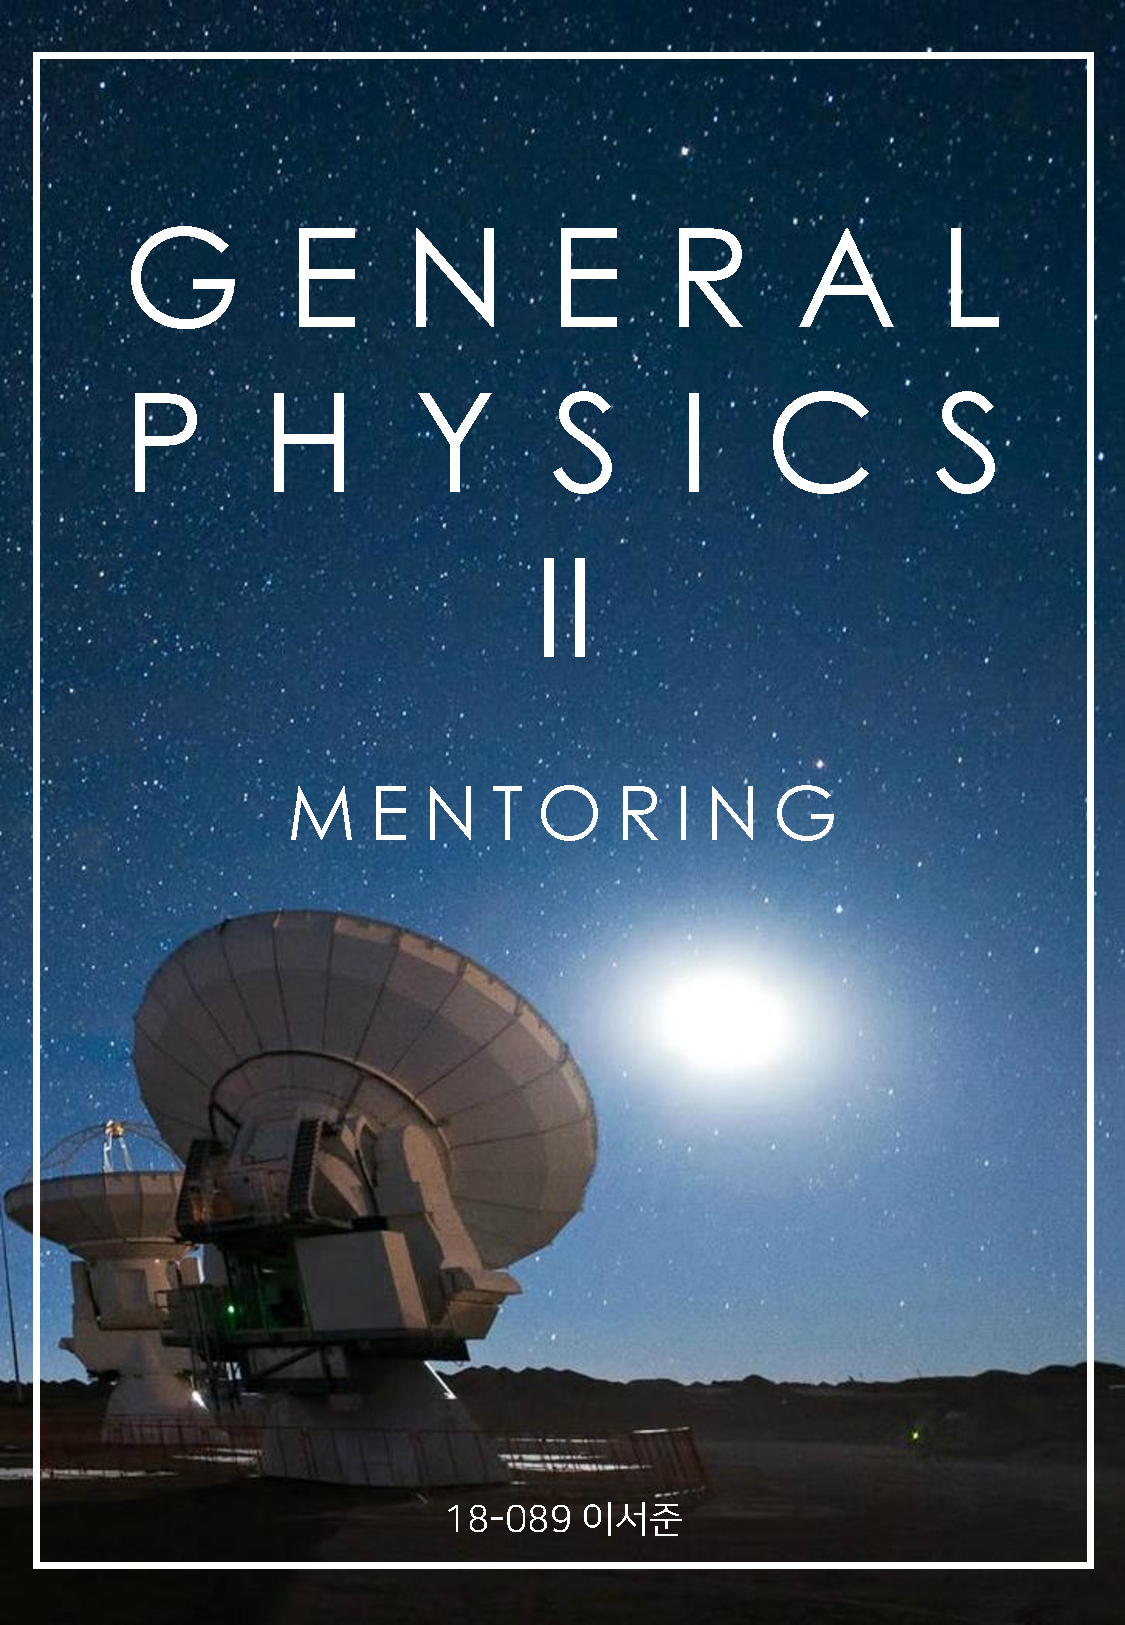
\includegraphics[width=\paperwidth]{title_page.pdf}};
%\draw (current page.center) node [fill=ocre!30!white,fill opacity=0.6,text opacity=1,inner sep=1cm]{\Huge\centering\bfseries\sffamily\parbox[c][][t]{\paperwidth}{\centering General Physics 2\\[15pt] % Book title
%{\huge Mentoring}\\[20pt] % Subtitle
%{\Large 18-089 이서준}}}; % Author name
\end{tikzpicture}
\vfill
\endgroup

%----------------------------------------------------------------------------------------
%	서문
%----------------------------------------------------------------------------------------

\newpage

\thispagestyle{empty}
\begin{center}
\noindent\huge{\textbf서문}}
\end{center}\\
\vspace{30pt}
\\
우리 한국과학영재학교가 다른 학교와 다르게 가지는 차별점은 학생들이 학원에 크게 의존하지 않고 자기주도적으로 공부를 해나간다는 점일 것입니다. 그러나 우리 학교의 일반물리학 과목의 경우 1학년 때 배웠던 물리에 비해 창의적인 발상이나 스킬을 요구하는 등 급격하게 난이도가 올라가 어려움을 겪는 학생들이 많습니다. 또한 교과서에 나와 있는 문제들과 실제 시험에서 출제되는 문제들의 난이도 차이가 크기 때문에 공부할 자료가 많지 않고, 선생님에 따라서 가르치시는 스타일에 확연한 차이가 있어 공부하는 데 많은 어려움이 있습니다.  이에 일반물리학을 수강하는 학생들이 스스로 공부할 수 있는 자료가 필요하다는 생각에 멘토링을 시작하게 되었고, 이 자료를 만들게 되었습니다.\\
이 멘토링 교재는 중간고사 범위로 정전기학과 정자기학, 그리고 회로이론의 3장, 기말고사 범위로 전자기파와 파동광학, 상대성 이론, 그리고 양자역학의 4장으로 구성되어 있습니다. 각 장에는 일반물리학2 수업을 진행하시는 두 분의 선생님께서 중점적으로 강조하신 부분을 모두 담으려고 최대한 노력하였습니다. 또한 교과서에 나와있지 않지만 헷갈릴 수 있거나 두 선생님의 수업에서 나왔던 내용을 담았습니다. 연습문제의 경우는 교과서(Bauer)와 그리피스 기초전자기학, 할리데이 일반물리학과 Irodov의 Problems in General Physics 등에서 직접 풀어보면서 어느 정도 난이도가 높고 풀어봐야 할 가치가 크다고 생각되는 것들을 골라 넣었습니다. 
또, 여러 분의 선배님들께서 멘토링 아카이브에 남겨 주신 기출 문제를 각 단원에 나누어 수록하였습니다. 만약 자료에 틀린 부분이 있다고 생각된다면 언제든지 정말 부담없이 \texttt{leeseojune89@gmail.com}으로 연락해 주시면 좋겠습니다.\\
마지막으로 소중한 기회를 제공해준 과학봉사부에 감사의 말씀을 드리고 싶습니다. 또, 제 멘토링을 수강한 9명의 학생들을 포함해서 이번 학기에 일반물리학2를 수강하는 모든 학생들이 만족스러운 성적을 거두기를 바라겠습니다!
\vfill~
\hfill~ 2020년 7월, 18-089 이서준 드림

%----------------------------------------------------------------------------------------
%	TABLE OF CONTENTS
%----------------------------------------------------------------------------------------

%\usechapterimagefalse % If you don't want to include a chapter image, use this to toggle images off - it can be enabled later with \usechapterimagetrue

\chapterimage{chapter_head_1(1).pdf} % Table of contents heading image

\pagestyle{empty} % Disable headers and footers for the following pages

\tableofcontents % Print the table of contents itself

\cleardoublepage % Forces the first chapter to start on an odd page so it's on the right side of the book

\pagestyle{fancy} % Enable headers and footers again

%----------------------------------------------------------------------------------------
%	PART
%----------------------------------------------------------------------------------------

\part{중간고사 범위}

%----------------------------------------------------------------------------------------
%	CHAPTER 1
%----------------------------------------------------------------------------------------

\chapterimage{chapter_head_2(1).pdf} % Chapter heading image

\chapter{정전기학}
전기역학에서 다루고자 하는 근본적인 문제는 원천 전하가 있을 때 시험 전하가 받는 힘을 구하는 것이다. 그런데 이는 각 전하의 전하량이나 위치뿐만 아니라, 각 전하의 속도나 가속도에 따라서도 달라지며 일반물리학의 범위에서 풀기 어렵다. 정전기학이란 시험전하는 움직일 수 있으나 원천전하는 고정된 특별한 경우에 관한 것으로, 교과서(Bauer)의 21-24장이 여기에 해당한다.\\
먼저 21장에서는 정전기학의 기본이 되는 쿨롱 법칙과 중첩 원리를 다루고, 이를 통해 시험전하가 받는 힘을 계산하는 방법을 배운다. 22장에서는 전기장을 정의하고, 연속적인 물체가 만드는 전기장을 적분을 사용하여 구하는 방법을 다룬다. 또한 가우스 법칙을 통해 대칭이 있는 상황에서의 전기장을 구하며 영상 전하법이라는 방법을 배운다.\\
23장에서는 전위에 대해 다루고, 전위와 전기장의 관계를 미적분을 사용해 배운다. 또한 연속적인 물체가 만드는 전위를 계산하는 방법을 배운다. \\
마지막으로 24장은 축전기에 대해서 배우는 단원으로, 앞서 배운 내용을 토대로 평행판 축전기뿐만 아니라 원통, 구형 등 다양한 형태의 축전기에 대해 다룬다. 또한 축전기의 직렬, 병렬 연결에 대한 내용과 함께 유전체에 관한 내용을 포함한다.\\
%------------------------------------------------

\section{전기장과 전위}
\begin{theorem}[쿨롱 법칙]
시험전하 $q$가 $\vec{r'}$에 위치하여 있을 때, $\vec{r}$에서의 전기장은
\begin{equation}
\vec{E}=\frac{q}{4\pi\epsilon_0}\frac{\vec{r}-\vec{r'}}{|\vec{r}-\vec{r'}|^3}
\end{equation}
이다. 이때 $\epsilon_0=8.85\times10^{-12}\mathrm{F/m}$는 진공에서의 유전율을 의미한다.
\end{theorem}

\begin{theorem}[전기장과 전위의 관계]
전기장을 $\vec{E}$, 전위를 $V$라고 할 때
\begin{equation}
\vec{E} = -\nabla V
\end{equation}
이다. 또한, 
\begin{equation}
\Delta V = V_f - V_i = -\int_i ^ f \vec{E} \cdot d\vec{l}
\end{equation}
이 성립한다.
\end{theorem}
전기장과 전위에 대해서는 중첩 원리가 적용된다. 즉, 여러 개의 전하가 만드는 전기장이나 전위는 각각이 만드는 전기장이나 전위의 벡터합과 같다. 이를 이용해 적분을 통해서 연속적인 전하 분포가 만드는 전기장과 전위를 구할 수 있다.
\begin{example}
길이 $2L$인 도선 토막에 전하가 선밀도 $\lambda$로 고르게 퍼져 있을 때, 중심에서 위쪽으로 거리 $z$인 곳의 전기장을 구하여라.(Bauer)
\end{example}
도선이 $x$축에 놓여 있다고 생각하고, 중심이 원점에 오도록 하자. 도선의 $x$에서 $x+dx$까지의 부분은 전하량이 $dq = \lambda dx$이다. 따라서 이 부분이 만들어내는 미소 전기장은 
\begin{equation}
d\vec{E}=\frac{\lambda dx}{4\pi\epsilon_0}\frac{-x\hat{x}+z\hat{z}}{(x^2+z^2)^{3/2}}
\end{equation}
이다. 그런데, $\hat{x}$ 성분은 $-x$에서 $-(x+dx)$까지에 해당하는 부분에 의해 상쇄된다. 따라서 $\hat{z}$방향 성분만 계산해주면 된다. 그러므로
\begin{align}
E_z &= \int_{-L}^L \frac{1}{4\pi\epsilon_0}\frac{z\lambda dx}{(x^2+z^2)^{3/2}}\\
&=\int_{-\tan^{-1}(L/z)}^{\tan^{-1}(L/z)} \frac{1}{4\pi\epsilon_0}\frac{z^2\lambda\sec^2 \theta d\theta }{z^3 \sec^3 \theta} \quad(x=z\tan\theta, dx=z\sec^2\theta d\theta)\\
&= \int_{-\tan^{-1}(L/z)}^{\tan^{-1}(L/z)} \frac{1}{4\pi\epsilon_0}\frac{\lambda\cos \theta d\theta }{z}\\
&=\frac{\lambda}{4\pi\epsilon_0z}[\sin\theta]_{-\tan^{-1}(L/z)}^{\tan^{-1}(L/z)} \\
&= \frac{\lambda L}{2\pi\epsilon_0z\sqrt{z^2+L^2}{}}
\end{align}
임을 알 수 있다. \\
\begin{exercise}
비슷한 방법으로 위 상황에서 전위를 구하여라.
\end{exercise}

\paragraph{전기 쌍극자 모멘트} 전하가 각각 $+q$와 $-q$인 두 전하가 $d$만큼의 거리를 두고 떨어져 있을 때, 이 전하분포의 전기 쌍극자 모멘트는 $\vec{p}=q\vec{d}$이며, $\vec{d}$의 방향은 $-q$에서 $+q$를 향하는 방향이다. 전기 쌍극자가 균일한 전기장 $\vec{E}$ 안에 있을 때, 이것이 받는 토크는 $\vec{\tau}=\vec{p}\times \vec{E}$이며, 퍼텐셜에너지는 $U=-\vec{p} \cdot \vec{E}$이다. 참고로 전기 쌍극자가 균일하지 않은 전기장에 있을 때는 알짜힘이 0이 아니게 되며, $\vec{F}=(\vec{p}\cdot \nabla)\vec{E}$로 계산된다.\\
전기 쌍극자가 만드는 전위는 
\begin{equation}\label{eqn: elecdipole}
\vec{E} = \frac{1}{4\pi\epsilon_0}\frac{p\cos\theta}{r^2}
\end{equation}
이다. 이때 $\theta$는 전위를 측정하는 지점의 벡터 $\vec{r}$과 $\vec{p}$가 이루는 각이다. 
\begin{exercise}
전기 쌍극자가 받는 토크가 $\vec{\tau}=\vec{p}\times \vec{E}$임을 이용하여 이것의 퍼텐셜 에너지를 유도하여라.
\end{exercise}

\begin{exercise}
$+q$의 전하가 $(0,0,d/2)$에, $-q$의 전하가 $(0,0,-d/2)$에 놓여 있는 전기 쌍극자가 있다. $\vec{r}$의 위치에서의 전위가 식 \ref{eqn: elecdipole}와 같이 표현됨을 보여라.(힌트: 두 전하와의 거리를 $r_+$와 $r_-$라고 하고, $r_+r_-$와 $r_+-r_-$를 각각 근사하여라.)
\end{exercise}

\begin{problem}
반지름이 $r$인 둥근 고리에 전하가 선밀도 $\lambda$로 퍼져 있을 때, 고리 중심에서 위쪽으로 거리 $z$인 곳의 (1)전기장과 (2)전위를 구하라. (Griffiths)
\end{problem}

\begin{problem}
위 문제의 결과를 이용하며 반지름이 $r$인 원반에 전하가 면밀도 $\sigma$로 퍼져있을 경우, 중심에서 위쪽으로 거리 $z$인 곳의 (1)전기장과 (2)전위를 구하라. (힌트: 반지름이 $r$에서 $r+dr$인 고리는 선밀도가 $\lambda=\sigma dr$이라고 볼 수 있다.)
\end{problem}

\begin{problem}\label{2014-2(1)}
\begin{figure}[h]
\centering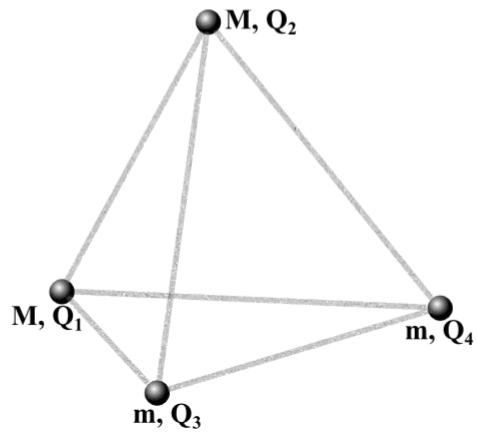
\includegraphics[scale=0.4]{Pictures/2014-2(1).PNG}
\caption{Problem \ref{2014-2(1)}}
\label{fig:2014-2(1)}
%\addcontentsline{toc}{figure}{Figure \ref{fig:placeholder}} % Uncomment to add the figure to the table of contents
\end{figure}
Figure \ref{fig:2014-2(1)}과 같이 점전하들이 배치되어 있으며, 각 전하는 다른 전하와 막대로 연결되어 있다. $q_3$와 $q_4$를 연결하는 막대가 끊어졌을 때, 모든 전하가 한 평면에 오는 순간 각 전하의 속도를 구하여라. (2014-2 기출)
\end{problem}

\begin{problem}\label{2014-1(5)}
도체 고리가 $q$로 균일하게 대전되어 있으며, 고리의 축을 따라 $L$만큼 떨어진 거리에 전하 $-q$, 질량 $m$인 물체가 놓여 있다. (1) 물체가 고리의 중심을 지날 때 갖는 운동에너지 (2) 물체가 축을 따라 단진동할 때 주기를 구하여라. 단, $R\gg L$이다. (2014-1 기출)
\end{problem}

\begin{problem}\label{2015-1(1)}
\begin{figure}[h]
\centering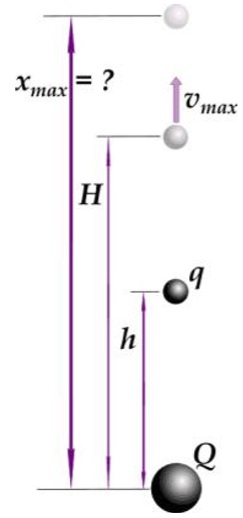
\includegraphics[scale=0.5]{Pictures/2015-1(1).PNG}
\caption{Problem \ref{2015-1(1)}}
\label{fig:2015-1(1)}
%\addcontentsline{toc}{figure}{Figure \ref{fig:placeholder}} % Uncomment to add the figure to the table of contents
\end{figure}
Figure \ref{fig:2015-1(1)}과 같이 전하 $Q$가 고정되어 있으며 다른 전하는 $h$의 위치에 정지해 있다가 낙하한다. 이 전하는 낙하하다가 $H>h$의 위치에서 속도가 최고가 된다. 이때 이 전하가 올라갈 수 있는 최고점의 높이는 얼마인가? (2015-1 기출)
\end{problem}

\begin{problem}
한 변의 길이가 $2L$인 정사각형에 전하가 면밀도 $\sigma$로 퍼져있다. 이때 중심에서 위쪽으로 거리 $z$인 곳의 전위를 구하라. (퀴즈 기출)
\end{problem}

\begin{problem}
만유인력에서, 구껍질이 바깥에 있는 물체에 작용하는 만유인력의 크기는 같은 질량이 구껍질의 중심에 있을 때 물체에 작용하는 만유인력의 크기와 같다. 이를 뉴턴의 구각정리라고 한다. 정전기력에 대해 구각 정리를 증명하여라. 즉, $q$만큼의 전하가 골고루 퍼져있는 구껍질이 바깥의 점전하에 작용하는 정전기력이 구껍질의 중심에 같은 크기의 전하가 있을 때 작용하는 정전기력과 같음을 보여라.
\end{problem}

\section{가우스 법칙}
\begin{theorem}[가우스 법칙]
어떤 폐곡면 $S$에 대해, $S$ 안에 들어있는 전하의 총량을 $q$라고 하면 
\begin{equation}
\oint_S \vec{E}\cdot d\vec{a}=\frac{q}{\epsilon_0}
\end{equation}
이 성립한다. 
\end{theorem}
가우스 법칙은 특히 원통이나 구대칭이 존재하는 문제에서 유용하게 사용된다.

\begin{example}[원통 대칭]
무한 도체 도선에 전하가 선전하밀도 $\lambda$로 고르게 대전되어 있다. 이 도선에서 반지름 방향으로 $r$만큼 떨어진 위치에서의 전기장을 구하여라.
\end{example}
길이가 $l$이고, 반지름이 $r$이며 도체 도선이 축인 원통을 가우스 면으로 잡자. 그러면 $\oint \vec{E}d\vec{a}=E\cdot(2\pi r l)=\frac{\lambda l}{\epsilon_0}$이고 반지름 방향이므로 $\vec{E}=\frac{\lambda}{2\pi r\epsilon_0}\hat{r}$임을 알 수 있다.\\

\begin{example}[평면 대칭]
무한 평면에 전하가 면전하밀도 $\sigma$로 고르게 대전되어 있다. 이 평면에서 $d$만큼 떨어진 지점에서의 전기장을 구하여라.
\end{example}
무한 평면이 중심을 지나는, 양 면이 무한 평면에 평행한 원통을 생각하자. 양 면의 넓이는 $A$이다.  이때 $\oint \vec{E}d\vec{a}=2E\cdot A=A\sigma /\epsilon_0$이므로 $E=\sigma/\epsilon_0 \hat{n}$임을 알 수 있다.


\begin{exercise}[구면 대칭]
반지름이 $a$인 부도체 공에 전하가 $\rho$의 부피전하밀도로 균일하게 대전되어 있다. $r<a$일 때와 $r>a$일 때 전기장의 세기를 구하여라.
\end{exercise}

\begin{problem}\label{2014-1(3)}
\begin{figure}[h]
\centering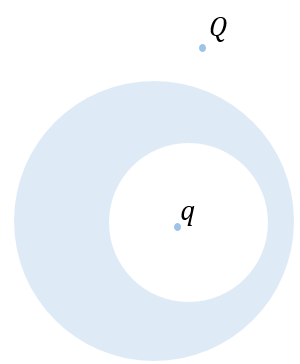
\includegraphics[scale=0.5]{Pictures/2014-1(3).PNG}
\caption{Problem \ref{2014-1(3)}}
\label{fig:2014-1(3)}
%\addcontentsline{toc}{figure}{Figure \ref{fig:placeholder}} % Uncomment to add the figure to the table of contents
\end{figure}
Figure \ref{fig:2014-1(3)}과 같이 공동이 있는 도체 내부와 외부에 각각 전하 $q$와 $Q$가 위치해 있다. (1) 도체의 바깥쪽과 안쪽 표면의 전하량 (2) $Q$를 조금 움직였을 때 각 표면의 전하 배치의 변화 (3) $q$를 조금 움직였을 때 각 표면의 전하 배치의 변화 (4) $Q$와 $q$에 작용하는 힘을 쓰시오. (2014-1 기출)
\end{problem}

\begin{problem}\label{2015-1(2)}
\begin{figure}[h]
\centering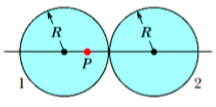
\includegraphics[scale=1.0]{Pictures/2015-1(2).PNG}
\caption{Problem \ref{2015-1(2)}}
\label{fig:2015-1(2)}
%\addcontentsline{toc}{figure}{Figure \ref{fig:placeholder}} % Uncomment to add the figure to the table of contents
\end{figure}
Figure \ref{fig:2015-1(2)}와 같이 반지름이 $R$인 부도체 구 2개에 각각 전하가 고르게 분포되어 있다. 두 구의 중심을 잇는 선분 위의, 첫 번째 구에서 $R/2.00$만큼 떨어진 지점에 $P$가 위치해 있다. (1) $P$에서 알짜 전기장이 0이라면, 두 구에 대전된 전하량의 비는 얼마인가? (2) 두 구의 접점에서 전기장은 얼마인가? (2015-1 기출)

\end{problem}

\section{영상전하법}
다음 문제를 보자.
\begin{example}
접지된 무한 도체 평판 위 거리 $d$인 곳에 전하량 $q$의 점전하가 있다. 이때 점전하가 만들어내는 전기장에 의해 도체 평판에는 - 전하가 유도되며, 이에 따라 전하에는 아래 방향의 인력이 작용하게 된다. 이때 평판 위 임의의 위치에서 전기장을 구하고, 점전하가 받는 인력과 계의 에너지를 구하여라.\label{imagecharge}
\begin{figure}[h]
\centering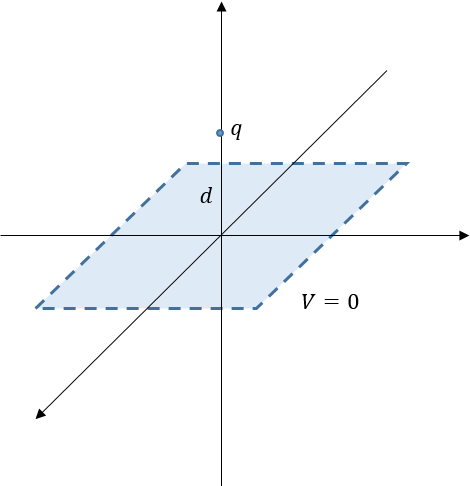
\includegraphics[scale=0.5]{Pictures/image_charge-1.PNG}
\caption{무한 도체 평면과 점전하}
%\addcontentsline{toc}{figure}{Figure \ref{fig:placeholder}} % Uncomment to add the figure to the table of contents
\end{figure}

\end{example}
이러한 문제를 풀 때 사용할 수 있는 방법이 \textbf{영상전하법}(image charge method)이다. 위의 문제는 영상전하법을 사용하여 Figure \ref{fig: imagecharge2}와 같이 바꾸어 생각할 수 있다.
\begin{figure}[h]
\centering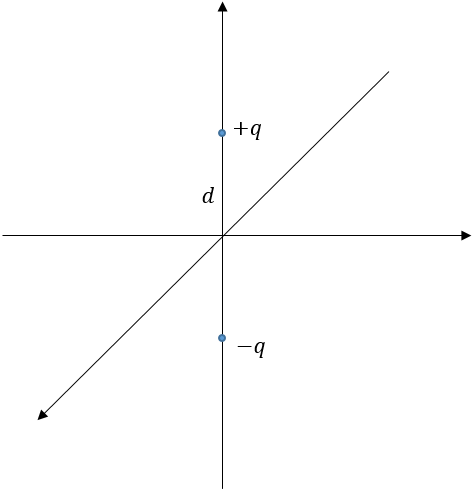
\includegraphics[scale=0.5]{Pictures/image_charge-2.PNG}
\label{fig: imagecharge2}
\caption{무한 도체 평면과 점전하}
%\addcontentsline{toc}{figure}{Figure \ref{fig:placeholder}} % Uncomment to add the figure to the table of contents
\end{figure}
이것이 가능한 이유는 특정 영역에서의 전위를 구하는 문제는 곧 푸아송 방정식 $\nabla^2 V = -\frac{\rho}{\epsilon_0}$를 푸는 것과 같기 때문이다. 따라서 우리가 '관심 있는 영역'(위의 문제에서는 $z>0$인 영역)에서의 전하 분포가 같고, 경계 조건(위의 문제에서는 $z=0$인 곳과 $r\to\infty$일 때 $V=0$이라는 것)이 같다면 특정 상황에서 전위를 구하는 문제를 다른 상황으로 바꾸어 생각할 수 있다. 두 상황에서 $xy$평면의 전위는 모두 $V=0$으로 같으며, 무한히 먼 지점에서의 전위도 $V=0$으로 같다. 따라서 문제의 상황을 위의 그림과 같이 바꿀 수 있는 것이다. \\
\begin{exercise}
Example \ref{imagecharge}을 풀어라.
\end{exercise}
영상전하법을 이용한 후 계의 에너지를 구할 때는 구한 이미지에 $1/2$을 곱해주어야 한다는 점에 유의해야 한다. 즉, 위의 상황에서 에너지는 $-\frac{1}{4\pi\epsilon_0}\frac{q^2}{2d}$이 아니라 이것의 절반인 $-\frac{1}{8\pi\epsilon_0}\frac{q^2}{2d}$이 된다. 이는 계의 상호작용 에너지가 $\int_{전 공간} \epsilon_0\vec{E_1}\cdot\vec{E_2} d\tau$로 계산되고, 적분을 하는 공간이 영상전하법을 쓴 경우에는 원래 상황의 2배가 되어버리기 때문이다. 따라서 반드시 $1/2$를 곱해야 하는 것은 아니며, Problem\label{image_charge_4}와 같은 상황에서는 영상전하법을 사용하여 에너지를 구한 후 $1/4$를 곱해야 한다.
영상전하법은 평면뿐만 아니라 접지된 도체 공의 경우에도 적용될 수 있다.
\begin{example} \label{ic4}
\begin{figure}[h]
\centering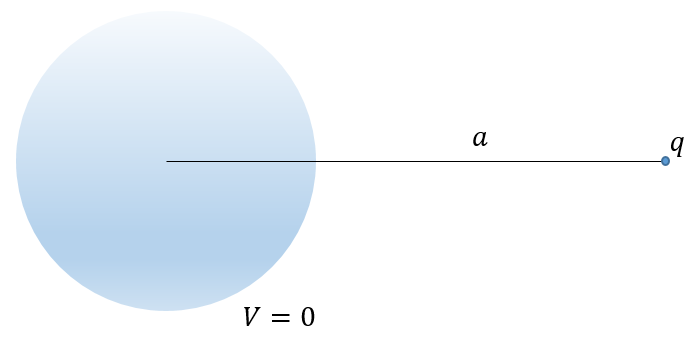
\includegraphics[scale=0.5]{Pictures/image_charge-4.PNG}
\caption{접지된 도체 공 외부의 점전하}
%\addcontentsline{toc}{figure}{Figure \ref{fig:placeholder}} % Uncomment to add the figure to the table of contents
\end{figure}
위와 같이 반지름이 $R$인 접지된 도체 공의 중심에서 $a$만큼 떨어진 지점에 전하량이 $q$인 점전하가 위치해 있다. (1)이 전하가 받는 인력의 크기 (2)도체 표면에서의 전기장의 크기 (3)공에 유도된 전하량을 구하여라.
\end{example}

위의 경우는 아래 그림과 같이 바꾸어 생각할 수 있다.
\begin{figure}[h]
\centering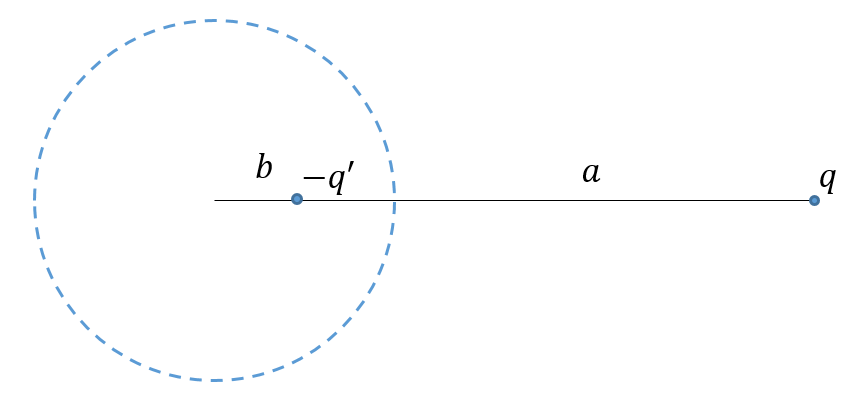
\includegraphics[scale=0.4]{Pictures/image_charge-5.PNG}
\caption{Example \ref{ic4}}
%\addcontentsline{toc}{figure}{Figure \ref{fig:placeholder}} % Uncomment to add the figure to the table of contents
\end{figure}
즉, 중심에서 $b$만큼 떨어진 지점에 $-q'$의 전하를 두어 구껍질에서의 전위가 0이 되도록 하면 되는 것이다. 따라서 전하 $q$와 $-q'$에서 구각 위의 특정 지점을 잇는 벡터를 각각 $\vec{r_1}, \vec{r_2}$라고 할 때 $k\frac{q}{r_1}-k\frac{q'}{r_2}=0$이 성립하며, 이에 따라 
\begin{equation}
\frac{q'}{q}=\frac{r_2}{r_1}=\frac{R-b}{a-R}=\frac{R+b}{R+a}
\end{equation}
가 성립한다. 가비의 리를 사용하면 $b=R^2/a$이고 $q'=\frac{R}{a}q$임을 알 수 있다. 따라서 전하가 받는 힘의 크기는 $F=k\frac{qq'}{(a-b)^2}=k\frac{Rq^2/a}{(a-R^2/a)^2}$이다.
전기장은 두 전하가 만드는 전기장의 중첩으로 구할 수 있다. 구의 중심에서 구각의 특정 위치를 잇는 벡터를 $\vec{r}$, 중심에서 점전하를 향하는 방향 벡터를 $\hat{z}$라고 하면
\begin{align}
\vec{E}&=k\frac{q\vec{r_1}}{r_1^3}+k\frac{-q'\vec{r_2}}{r_2^3}\\
&=k\frac{q(r\hat{r}-b\hat{z})}{(r^2+a^2-2ra\cos\theta)^{3/2}}-k\frac{q'(r\hat{r}-b\hat{z})}{(r^2+b^2-2rb\cos\theta)^{3/2}}
\end{align}
임을 알 수 있다. 또한 가우스 법칙에 의해 $E_r = \sigma/\epsilon_0$이므로 이를 통해 표면전하의 밀도를 구할 수 있다.
\begin{align}
E_r &= \hat{r} \cdot \vec{E} = \sigma /\epsilon_0\\
&= k\frac{qr-qa\cos\theta}{(r^2+a^2-2ra\cos\theta)^{3/2}}-k\frac{r/a\cdot q(r-r^2/a\cdot \cos\theta)}{(r^2+(r^2/a)^2-2r(r^2/a)\cos\theta)^{3/2}}\\
&= k\frac{q\{(R-a\cos\theta)-(a^2/R-a\cos\theta)\}}{(r^2+a^2-2ra\cos\theta)^{3/2}}\\
&= k\frac{q(R-a^2/R)}{(r^2+a^2-2ra\cos\theta)^{3/2}}
\end{align}
따라서 면전하밀도는 
\begin{equation}
\sigma = -\frac{q(R-a^2/R)}{4\pi(r^2+a^2-2ra\cos\theta)^{3/2}}
\end{equation}임을 알 수 있다. 유도된 전하의 양을 구하기 위해서는 이를 적분하면 된다.
$\hat{z}$와 이루는 각이 $\theta$와 $\theta+d\theta$ 사이인 영역의 넓이는 $dA = 2\pi r^2 \sin\theta d\theta$ 이므로
\begin{align}
Q &= \int \sigma dA \\
&= -\int_0^\pi  -\frac{q(R-a^2/R)}{4\pi(r^2+a^2-2ra\cos\theta)^{3/2}} \cdot 2\pi R^2 \sin\theta d\theta \\
&= -\frac{qR(a^2-R^2)}{2}\int_0^\pi \frac{\sin\theta d\theta}{(r^2+a^2-2ra\cos\theta)^{3/2}}\\
&= \frac{qR(a^2-R^2)}{2} \int_{a-R}^{a+R} \frac{1/Ra \cdot sds}{s^3}\quad (s^2 = a^2 + R^2 -2aR\cos\theta)\\
&=-\frac{q}{2a}(a^2-R^2)\left [-\frac{1}{s}\right ]^{a+R}_{a-R}\\
&= -\frac{R}{a}q = -q'
\end{align}
즉, 구면에 유도된 전하량의 양은 영상전하의 크기와 같다. 조금만 생각하면 이것은 당연한 것임을 알 수 있는데, 원래의 상황에서 구로 들어가는 전기력선속의 합은 새로운 상황에서 전기력선속의 합과 같으며 가우스 법칙에 의해서 내부의 전하의 크기도 같기 때문이다.이 경우에는 에너지를 구한 후 얼마를 곱해야 하는지 생각하기 어려울 수 있으나, 계산을 해보면 무한 평면의 경우와 똑같이 절반을 곱하면 된다는 결론을 얻을 수 있다.
\begin{problem}\label{image_charge_4}
$x>0, y>0$인 영역에서 zx평면과 yz평면이 접지된 도체 판으로 이루어져 있고, $(a,b)$의 위치에 점전하 $+q$가 위치해 있다. 이때 영상전하를 어디에 배치해야 할지 생각하고 이 점전하가 받는 힘의 크기를 구하여라. (Griffiths) 
\end{problem}

\begin{problem}\label{2016-1}
\begin{figure}[h]
\centering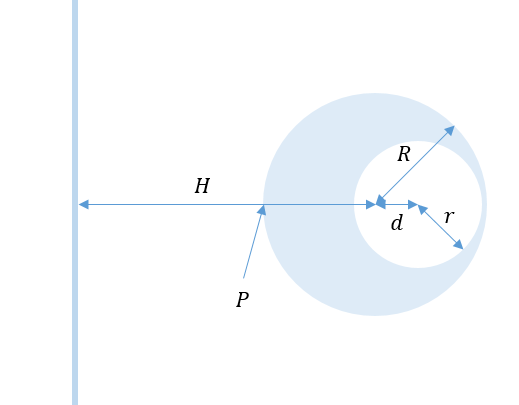
\includegraphics[scale=0.6]{Pictures/2016-1.PNG}
\caption{Problem \ref{2016-1}}
\label{fig:2016-1} % Unique label used for referencing the figure in-text
%\addcontentsline{toc}{figure}{Figure \ref{fig:placeholder}} % Uncomment to add the figure to the table of contents
\end{figure}
Figure \ref{fig:2016-1}과 같이 반지름이 $R$인 부도체 구가 $\rho$의 부피전하밀도로 대전되어 있고, 그 안에는 반지름이 $r$인 구멍이 있다. 또한 구의 중심에서 $H$만큼 떨어진 곳에는 무한한 도체 평면이 접지되어 있다. (1) 이 물체가 평면으로부터 받는 힘 (2) $P$ 지점에서의 전위 (3) 이 물체를 제자리에서 180\degree 회전시키는 데 드는 일 (4) 무한 평면의 각 위치에서의 면전하밀도를 구하여라. (2016-1 기출) 
\end{problem}

\begin{problem}\label{ic3}
\begin{figure}[h]
\centering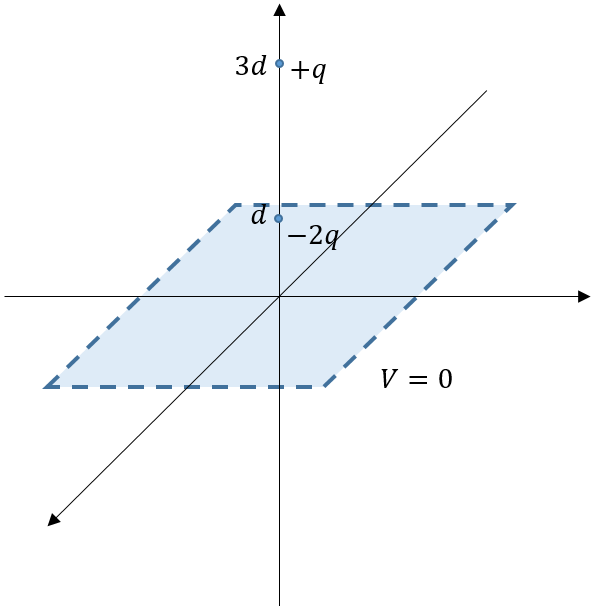
\includegraphics[scale=0.4]{Pictures/image_charge-3.PNG}
\caption{Problem \ref{ic3}}
\label{fig:ic3} % Unique label used for referencing the figure in-text
%\addcontentsline{toc}{figure}{Figure \ref{fig:placeholder}} % Uncomment to add the figure to the table of contents
\end{figure}
Figure \ref{fig:ic3}의 상황에서 전하 +q가 받는 힘을 셈하라. (Griffiths)
\end{problem}

\section{축전기}
\paragraph{축전기의 전기용량}
물리2에서는 평행판 축전기의 전기용량만을 다루었다. 그러나 일물2에서는 원통이나 구형 축전기의 전기용량을 구하는 방법도 배운다. 다음 예제를 보자.
\begin{example}[평행판 축전기]
각 금속 판의 면적이 $A$이고 두 판 사이의 간격이 $d$인 평행판 축전기의 전기용량을 구하라(단, 두 판 사이는 진공으로 채워져 있다.). 
\end{example}
답이 $C=\epsilon_0\frac{A}{d}$임은 이미 알고 있겠지만, 이 답이 왜 나온 것인지 생각해보자. 먼저, 각 판에  $+Q$와 $-Q$가 대전되어 있다고 가정하자. 이때 가우스 법칙을 통해 두 판 사이의 전기장의 세기는 $E=\sigma/\epsilon_0=Q/(\epsilon_0A)$임을 알 수 있다. $\Delta V=-\int_i^f \vec{E}\cdot d\vec{l}$이므로, 두 판 사이의 전위차는 $Qd/(\epsilon_0 A)$이다. 그런데 전기 용량은 $C=Q/V$로 정의되므로  $C=\epsilon_0 A/d$임을 알 수 있다.\\
이런 식으로 두 극판에 $+Q$와 $-Q$가 대전되었다고 가정한 후 가우스 법칙을 통해 전기장을 구하고, 이를 적분해서 전위차를 구하여 전기용량을 구할 수 있다. 
\begin{exercise}
안쪽 반지름이 $a$, 바깥쪽 반지름이 $b$인 길이 $l$짜리 원통형 축전기의 축전 용량이 
\begin{equation}
C=\frac{2\pi\epsilon_0l}{\ln{b/a}}
\end{equation}
임을 보여라.
\end{exercise}

\begin{exercise}
안쪽 반지름이 $a$, 바깥쪽 반지름이 $b$인 구형 축전기의 축전 용량을 구하여라.\label{spherecap}
\end{exercise}
축전기 안에 유전체가 있는 경우에도 전기 용량을 구할 수 있는데, 이는 다음 장에서 다루겠다.\\

\begin{problem}
Exercise \ref{spherecap}에서 $b\to\infty$로 보내 구의 축전 용량을 구할 수 있다. 이를 계산하라.
\end{problem}

\begin{problem}
반지름이 $a$인 평행한 두 긴 원통 모양의 직선 도선이 있다. 두 도선의 축 사이의 거리가 $b$일 때, 이 계의 단위길이당 전기용량을 구하여라. (Irodov)
\end{problem}

\begin{problem}
무한한 도체 평면에 평행하게 긴 원통 모양의 직선 도선이 있다. 이 도선의 반지름은 $a$이고 도선의 축에서 평면까지의 거리는 $b$이다. $a\ll b$일 때, 이 계의 단위길이당 전기용량을 구하여라. (Irodov)
\end{problem}

\section{유전체}



유전체는 전기장을 걸어주면 그 안의 전하가 정렬되면서 쌍극자가 전기장의 방향으로 늘어서는 물질이다. 이렇게 만들어진 쌍극자들은 전위나 전기장에 영향을 미치며, 그 영향은 유전체의 경계에 면전하가 분포하는 효과나 유전체 안에 실제 전하가 분포하는 효과와 같다. 이렇게 유전체가 편극됨으로써 생겨나는 전하를 \bold{속박전하}(bound charge)라고 한다. 이에 상대하여 실제 분포하는 전하를 자유전하(free charge)라고 한다.
속박전하가 존재하는 상황에서 전기장을 계산할 때는 주의할 점이 있다. 특히 가우스 법칙을 사용하여 계산할 때, 다음의 두 계산 방식 중 하나를 택해야 한다.
\begin{theorem}[유전체가 있을 때의 가우스 법칙]
유전체가 있는 상황에서 가우스 법칙을 적용할 때에는 다음 중 하나를 사용할 수 있다.
\begin{equation}\label{gauss1} \oint \vec{E} \cdot d\vec{a} = \frac{q_{f}+q_{b}}{\epsilon_0} \end{equation}
또는,
\begin{equation}\label{gauss2} \oint \vec{E} \cdot d\vec{a} = \frac{q_{f}}{\epsilon} \end{equation}
이때 $q_{f}$와 $q_{b}$는 각각 폐곡면 안의 자유전하와 속박전하의 양을 의미하며, $\epsilon_0$와 $\epsilon$은 각각 진공과 해당 물질 안에서의 유전율을 의미한다.
\end{theorem}
즉, 유전체를 아예 생각하지 않고 속박전하와 자유전하의 합, 즉 총 전하의 효과를 고려하거나, 유전체를 고려하면서 자유전하의 효과만을 포함해야한다는 것이다. 이를 생각하지 않고 유전율로 $\epsilon_0$를 사용하면서 자유전하만을 고려한다거나 유전율로 $\epsilon$을 사용하면서 자유전하와 속박전하를 모두 고려하여 계산한다면 잘못된 답을 얻게 된다.

\begin{example}
반지름이 $R$인 도체 공에 $Q$만큼의 전하가 대전되어 있고, 그 주위를 유전율이 $\epsilon=\kappa\epsilon_0$인 유전체가 둘러싸고 있다. 이때 도체 공과 유전체의 경계에 위치한 속박전하의 양을 구하여라.
\end{example}
속박전하의 양은 알지 못하고 자유전하의 양만을 알고 있는 상태이기 때문에 Equation \ref{gauss2}을 사용하여 전기장을 구할 수 있다. 그러면 $\vec{E}=\frac{Q}{4\pi r^2\epsilon}\hat{r}$임을 알 수 있는데, 이것은 Equation \ref{gauss1}을 사용하였을 때 얻는 결과와 같아야 하므로 $\frac{Q}{\epsilon}=\frac{Q}{\kappa\epsilon_0}=\frac{Q+q_b}{\epsilon_0}$이다. 따라서 $q_b = Q(-1+1/\kappa)$임을 알 수 있다.

\begin{exercise}\label{paracapa}
두 판의 넓이가 $A$이고 두 판 사이의 거리가 $d$인  평행판 축전기에 $Q$만큼의 전하가 저장되어 있고, 그 사이에는 유전율이 $\epsilon$인 유전체가 있다. 두 판 사이의 전기장을 위 두 방법을 각각 사용하여 구하고, 두 값이 같은지 확인하여라.
\end{exercise}
Exercise \ref{paracapa}를 해결한 후 전기 용량을 계산해 보면 전기용량은 $\epsilon\frac{A}{d}$가 된다는 것을 알 수 있을 것이다.

\begin{problem}
두 판 사이의 거리가 $2a$인 평행판 축전기에 윗부분에는 유전상수 $\kappa_1$, 두께 $a$인 유전체를, 아랫부분에는 유전상수가 $\kappa_2$, 두께가 $a$인 유전체판을 채워넣었다. 두 판의 면전하밀도가 $\sigma, -\sigma$일 때 (1)각 유전체판에서의 전기장 (2) 속박전하의 위치와 크기 (3) 두 극판 사이의 전위차 (4) 각 판의 면적이 $A$일 때 전기용량을 구하여라.
\end{problem}

\begin{problem}\label{dielec11}
\begin{figure}[h]
\centering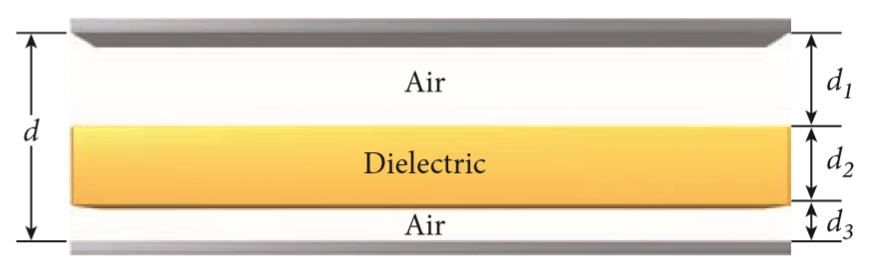
\includegraphics[scale=0.4]{Pictures/dielec11.PNG}
\caption{Problem \ref{dielec11}}
\label{fig:dielec11} % Unique label used for referencing the figure in-text
%\addcontentsline{toc}{figure}{Figure \ref{fig:placeholder}} % Uncomment to add the figure to the table of contents
\end{figure}
Figure \ref{fig:dielec11}과 같은 축전기가 있다. 두 금속판의 면적을 $A$라고 할 때 축전기의 전기용량을 구하고 이것이 유전체의 위치, 즉 $d_1$과 $d_3$에 의존하지 않는다는 것을 보여라. (Bauer)
\end{problem}

\begin{problem}\label{dielec-example2}
\begin{figure}[h]
\centering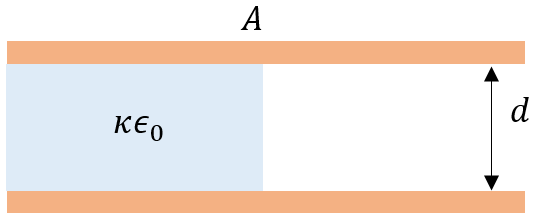
\includegraphics[scale=0.4]{Pictures/dielectric2.PNG}
\caption{Problem \ref{dielec-example2}}
\label{fig:dielec-example2} % Unique label used for referencing the figure in-text
%\addcontentsline{toc}{figure}{Figure \ref{fig:placeholder}} % Uncomment to add the figure to the table of contents
\end{figure}
Figure \ref{fig:dielec-example2}와 같이 평행판 축전기의 절반에 유전 상수 $\kappa$인 유전체를 채워넣었다. 이 축전기에 $V$의 전압을 걸었을 때, (1)각 영역에서 전기장의 세기 (2) 속박전하의 위치와 크기 (3) 전기 용량을 구하여라.
\end{problem}

\begin{problem}\label{dielec-example}
\begin{figure}[h]
\centering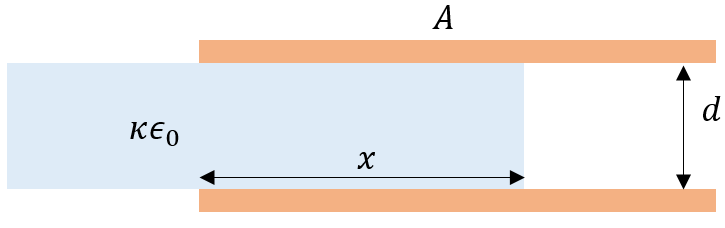
\includegraphics[scale=0.4]{Pictures/dielectric.PNG}
\caption{Problem \ref{dielec-example}}
\label{fig:dielec-example} % Unique label used for referencing the figure in-text
%\addcontentsline{toc}{figure}{Figure \ref{fig:placeholder}} % Uncomment to add the figure to the table of contents
\end{figure}
Figure \ref{fig:dielec-example}와 같이 길이 $l$, 간격 $d$, 넓이 $A$인 평행판 축전기에 넓이 $A$, 길이 $l$, 유전율 $\kappa\epsilon_0$인 유전체가 끼워져 있으나 길이 중 $x$만큼만이 축전기에 걸쳐져 있고 $l-x$만큼은 삐져나와 있다. 축전기에 저장된 전하량이 일정할 때, 이 유전체가 받는 힘을 구하여라. (힌트: $F=-dU/dx$임을 이용하라)
\end{problem}

\begin{problem}
이번에는 두 판 사이의 간격이 $d$인 평행판 축전기를 물(유전 상수 $\kappa$, 밀도 $\rho$)이 담긴 수조에 세워둔다. 또, 축전기에는 $V$의 전압을 걸어준다. 이때, Problem \ref{dielec-example}과 같은 이유로 물이 끌어올려지게 된다. 수면 위로 물이 올라간 높이가
\begin{equation}
x =\frac{V^2\epsilon_0(\kappa-1)}{2\rho g d^2}
\end{equation}
임을 보여라. 단, $g$는 중력가속도이다.
\end{problem}

\begin{problem}\label{dielec-example3}
\begin{figure}[h]
\centering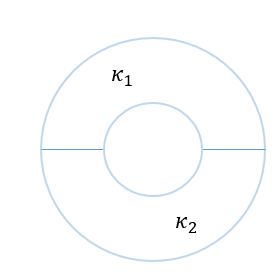
\includegraphics[scale=0.5]{Pictures/dielectric3.PNG}
\caption{Problem \ref{dielec-example3}}
\label{fig:dielec-example3} % Unique label used for referencing the figure in-text
%\addcontentsline{toc}{figure}{Figure \ref{fig:placeholder}} % Uncomment to add the figure to the table of contents
\end{figure}
Figure \ref{fig:dielec-example3}와 같은 안쪽 반지름 $a$, 바깥쪽 반지름 $b$인 무한히 긴 원통 축전기가 있다. 이 축전기의 위쪽 절반과 아래쪽 절반이 각각 $\kappa_1$과 $\kappa_2$의 유전상수를 갖는 유전체로 채워져 있다. (1) $q$만큼의 전하가 저장되었을 때 각 영역에서의 전기장 (2) 각 면에서의 속박전하의 양 (3) 축전기의 용량을 구하여라.
\end{problem}

%----------------------------------------------------------------------------------------
%	CHAPTER 2
%----------------------------------------------------------------------------------------
\chapter{정자기학}
\section{자기력}
\begin{theorem}[로렌츠 힘]
자기장이 $\vec{B}$인 곳에서 $q$의 전하가 $\vec{v}$의 속도로 운동할 때 받는 자기력의 크기는 $\vec{F_B}=q\vec{v}\times \vec{B}$이다.
자기력의 단위로는 테슬라(tesla, $T=\mathrm{N/(A\cdot m)}$)를 사용한다.
\end{theorem}
\begin{theorem}[자기장 속의 도선이 받는 힘]
$\vec{B}$의 자기장 속에 있는, 전류 $i$가 흐르는 길이 $l$인 도선이 받는 자기력은
$\vec{F}=i\vec{l}\times \vec{B}$이다. 이때 $\vec{l}$의 방향은 전류가 흐르는 방향과 같다.
\end{theorem}
균일한 자기장 안에서 전하가 속력 $v$로 발사된다면 자기력은 항상 속도에 수직한 방향으로 작용하기 때문에 원운동을 하게 된다. 이때 $\frac{mv^2}{r}=qvB$이므로 반지름은 $r=\frac{mv}{qB}$로 계산될 수 있다.

\begin{exercise} 
$\vec{B}=1.00\mathrm{T}\hat{z}$의 균일한 자기장이 작용하고 있는 영역이 있다. 이 공간에서 양성자($m_p=1.6726\times10^{−27}$, $+e=1.602\times 10^{-19}$C)가 $\vec{v_0}=(5.00\mathrm{m/s})\hat{x}+(0.50\mathrm{m/s})\hat{z}$의 속도로 발사되었다. 이때 (1) 양성자의 회전 주기 (2) 한 번의 주기에 $z$방향으로 진행한 거리를 구하여라. (2019-2 기출 유사)
\end{exercise}

\paragraph{자기 쌍극자 모멘트}
자기 쌍극자 모멘트는 다음과 같이 정의된다.
\begin{remark}
전류 $i$가 흐르는, $N$번 감긴 넓이 $A$인 고리의 자기 모멘트는 $\vec{\mu}=Ni\vec{A}$이다. 이때 $\vec{A}$의 방향은 고리의 법선 벡터 방향으로, 오른손 규칙을 따른다.
\end{remark}
자기 쌍극자가 균일한 자기장 속에서 받는 토크는 $\vec{\tau}=\vec{\mu}\times\vec{B}$이다. 또한 이에 의한 퍼텐셜 에너지의 크기는 $U=-\vec{\mu}\cdot\vec{B}$로 계산할 수 있다. 참고로 균일하지 않은 자기장에서는 자기 쌍극자가 받는 알짜힘이 0이 아니게 되며 그 값은 $\vec{F}=\nabla(\vec{\mu}\cdot\vec{B})$이다.
\begin{exercise}
자기 쌍극자가 받는 토크가 $\vec{\tau}=\vec{\mu}\times\vec{B}$임을 이용하여 자기 쌍극자의 퍼텐셜 에너지를 유도하여라.
\end{exercise}
일반물리학2에서는 적분을 이용하여 연속적인 물체의 자기 모멘트를 구하는 문제도 출제된다.
\begin{problem}
질량 $m$, 반지름 $R$의 원판에 전하 $q$가 균일하게 대전되어 있다. 이 원판이 중심을 지나는 축에 대해 각속도 $\omega$로 회전할 때 다음 물음에 답하시오. (1) 원판의 자기 모멘트 $\mu$는? (2) 자기 모멘트 $\mu$와 원판의 회전 운동량 $L$의 비는? (3) $q$의 부호는 $\mu$ 벡터와 $L$ 벡터의 방향에 어떠한 영향을 미치는가? (2014-1 기출)
\end{problem}
\begin{problem}
전하 $q$가 균일하게 대전되어 있는 반지름 $R$인 구가 있다. 이 구가 $\omega$의 각속도로 회전할 때, 자기 쌍극자 모멘트를 구하여라. 
\end{problem}
\begin{problem}
보어 모형에서 수소 원자의 반지름은 $r=5.29\times10^-11$ m이다. 이때 전자의 공전에 의해서 생기는 자기 쌍극자 모멘트의 크기를 구하여라. 또한, 전자의 각운동량을 구하여 쌍극자 모멘트와의 비를 계산하여라.
\end{problem}

\begin{problem}\label{2015-1(4)}
\begin{figure}[h]
\centering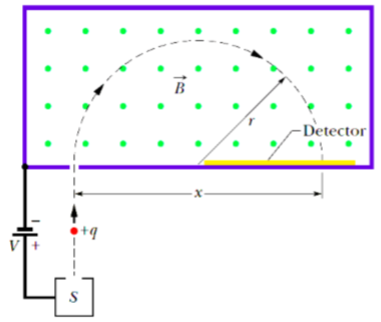
\includegraphics[scale=0.5]{Pictures/2015-1(4).PNG}
\caption{Problem \ref{2015-1(4)}}
\label{fig:2015-1(4)} % Unique label used for referencing the figure in-text
%\addcontentsline{toc}{figure}{Figure \ref{fig:placeholder}} % Uncomment to add the figure to the table of contents
\end{figure}
Figure \ref{2015-1(4)}와 같이 $3.92\times 10^{-25}$ kg의 질량과 $3.20\times 10^{-19}$ C의 전하를 가지는 우라늄 이온을 다른 이온과 분리하기 위한 질량 스펙트로미터가 있다. 시료들은 100 kV의 전위차로 가속된 후 균일한 자기장에 들어가 1.00 m의 반지름을 가지는 원호 형태의 경로를 따라 움직이게 된다. 180°만큼 움직인 후에는 폭 1.00 mm, 높이 1.00 cm인 슬릿을 통과한 후 컵에 모이게 된다. (1) 분리기 안의 수직 방향 자기장의 크기를 구하여라.[4점] (2) 이 장치를 통해 시간당 100 mg의 우라늄 이온을 분리하였다면, 이 이온의 운동에 따른 전류를 구하여라.[2점] (3) 1.00시간동안 생성된 열에너지를 구하여라.[2점]
(2015-1 기출)
\end{problem}

\section{비오-사바르 법칙}
전류가 만드는 자기장은 비오-사바르 법칙(Biot-Savart Law)을 통해 계산할 수 있다.
\begin{theorem}[비오-사바르 법칙]
$\vec{r'}$의 전류 $i$가 흐르는 도선의 $d\vec{s}$만큼의 부분이 $\vec{r}$의 위치에 만들어내는 미소 자기장은
\begin{equation}
d\vec{B} = \frac{\mu_0}{4\pi}\frac{id\vec{s}\times (\vec{r}-\vec{r'})}{|\vec{r}-\vec{r'}|^3}
\end{equation}와 같다.
\end{theorem}
이를 통해 여러 종류의 도선이 만들어내는 자기장을 계산할 수 있다.

\begin{example}[긴 직선 도선에 의한 자기장]\label{longwireB} 
$x$축을 따라 $i$만큼의 전류가 흐르는 긴 직선 도선이 있다. $(0,0,z)$에서의 자기장의 크기를 구하여라.
\end{example}
$x$에서 $x+dx$까지의 부분이 만들어내는 미소 자기장은 
\begin{align}
d\vec{B}&=\frac{\mu_0}{4\pi}\frac{i\langle dx,0,0\rangle \times \langle -x,0,z\rangle}{(x^2+z^2)^{3/2}}\\
&= \frac{\mu_0}{4\pi}\frac{-izdx\hat{y}}{(x^2+z^2)^{3/2}}
\end{align}
이다. 따라서,
\begin{align}
\vec{B} &= \int_{-\infty}^\infty \frac{\mu_0}{4\pi}\frac{-izdx\hat{y}}{(x^2+z^2)^{3/2}}\\
&= -\frac{\mu_0iz}{4\pi}\int_{-\infty}^\infty  \frac{dx}{(x^2+z^2)^{3/2}}\hat{y}\quad(x=z\tan\theta, dx = z\sec^2 \theta)\\
&= -\frac{\mu_0iz}{4\pi} \int_{-\pi/2}^{\pi/2} \frac{z\sec^2 \theta d\theta}{z^3 sec^3\theta}\hat{y}\\
&=-\frac{\mu_0i}{4\pi z} \int_{-\pi/2}^{\pi/2} \cos\theta \hat{y}\\
&= -\frac{\mu_0i}{2\pi z}\hat{y}
\end{align}
이 되는 것을 알 수 있다.
\begin{exercise}[원형 도선이 만드는 자기장]\label{circle}
반지름이 $a$인 원형 도선에 $i$만큼의 전류가 흐르고 있다. 이 도선에서 축 방향으로 $z$만큼 떨어진 지점의 자기장을 구하여라.
\end{exercise}

\begin{problem}
25.0 cm의 길이를 가지는 두 직선 도선이 4.00 mm 떨어져 있으며, 각각 9.00 V의 전압을 가지는 전지와 연결되어 있다. 첫 번째 도선의 저항이 5.00 Ω이고 다른 도선의 저항이 $R$일 때, 두 도선 사이에 작용하는 힘의 크기가 $4.00\cdot 10^{-5}$ N이 되도록 하는 저항 $R$의 크기를 구하여라. (Bauer)
\end{problem}

\begin{problem}
각도가 $\phi$인 원호 모양의 도선이 중심에 만드는 자기장을 구하고, $\phi = 2\pi$일 때 Exercise \ref{circle}이 $z=0$인 점에 만들어내는 자기장과 일치함을 확인하여라.
\end{problem}
\begin{problem}
(1) 모양이 $r(\theta)$의 극형식으로 주어지는 고리가 있다. 이 고리에 $i$의 전류가 흐를 때, 원점에 만들어지는 자기장의 크기가
\begin{equation}
B=\frac{\mu_0i}{4\pi}\oint \frac{d\theta}{r}
\end{equation}
임을 보여라. (힌트: $|d\vec{l}\times \hat{r}|=dl\sin\phi =rd\theta$임을 보여라. 단, $\phi$는 고리의 접선과 $\hat{r}$ 사이의 각도이다.) (2) $r(\theta)=a/\sqrt{\theta}(0< \theta \le 2\pi)$로 주어지는 모양을 리투스 나선(lituus spiral)이라고 한다. 이 도선이 원점에 만드는 자기장을 구하여라. (Griffiths)
\end{problem}

\begin{problem}
$(0,1,0)$을 지나며 $z$축과 평행한 도선에 $+z$ 방향으로 $I$=1A의 전류가 흐르고, $(0,2,0)$을 지나며 $x$축과 평행한 도선에 $+x$축 방향으로 같은 크기의 전류가 흐르고 있다. $(1.5, 1.5, 3)$에서의 자기장 $\vec{B}=\langle B_x, B_y, B_z \rangle$을 구하여라. (2014-1 기출)
\end{problem}

\begin{problem}\label{G5.26}
Figure \ref{fig:G5.26}과 같이 선전하밀도가 $\lambda$인 무한히 긴 도선 두 개가 $d$만큼 떨어져서 평행하게 놓여있다. 두 도선이 $v$의 속도로 움직일 때, 자기력이 전기력을 상쇄하기 위해서는 속도가 얼마나 빨라야 하는지 구하여라. (Griffiths)

\begin{figure}[h]
\centering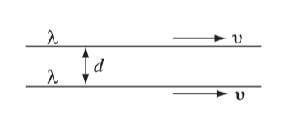
\includegraphics[scale=1.2]{Pictures/G5.26.eps}
\caption{Problem \ref{G5.26}}
\label{fig:G5.26} % Unique label used for referencing the figure in-text
%\addcontentsline{toc}{figure}{Figure \ref{fig:placeholder}} % Uncomment to add the figure to the table of contents
\end{figure}
\end{problem}

\begin{problem}\label{G5.25}
Figure \ref{fig:G5.25}와 같이 반지름이 $r$, 단위 길이당 감은 수가 $n$이고 전류가 $I$인 솔레노이드가 있다. 이 솔레노이드가 점 $P$에 만드는 자기장의 크기를 $\theta_1, \theta_2$로 나타내고, 두 각이 무한대가 될 때 자기장이 어떻게 될 지 생각해보라.(Griffiths)
\begin{figure}[h]
\centering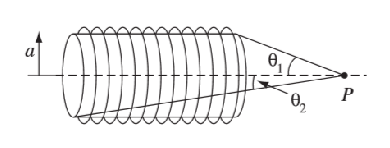
\includegraphics[scale=1.2]{Pictures/G5.25.eps}
\caption{Problem \ref{G5.25}}
\label{fig:G5.25} % Unique label used for referencing the figure in-text
%\addcontentsline{toc}{figure}{Figure \ref{fig:placeholder}} % Uncomment to add the figure to the table of contents
\end{figure}
\end{problem}

\section{앙페르 법칙}
원통 대칭과 같은 대칭이 존재하는 경우에는 비오-사바르 법칙 대신 앙페르 법칙을 사용하여 자기장을 구할 수 있다.
\begin{theorem}[앙페르 법칙]
어떤 폐곡선 $C$를 통과하는 전류의 크기가 $i_{enc}$일 때, 
\begin{equation}
\oint_C \vec{B}\cdot d\vec{s} = \mu_0i_{enc}
\end{equation}이다.
\end{theorem}

\begin{example}[긴 직선 도선에 의한 자기장]
반지름이 $R$인 긴 직선 도선에 전류 $i$가 $+z$ 방향으로 고르게 흐르고 있다. 도선의 축에서 $r$만큼 떨어진 지점에서의 자기장을 구하여라.
\end{example}
대칭에 의해 도선에서 같은 거리만큼 떨어진 부분에서 자기장은 일정할 것이다. 또한, 자기장에는 반지름 방향의 성분이 없다는 것은 이미 알고 있다. 먼저 $r<R$일 때,
\begin{equation}
B(2\pi r) = \mu_0 i_{enc}=\mu_0 i\left (\frac{r}{R}\right)^2
\end{equation}
이므로 $\vec{B}=\frac{\mu_0ir}{2\pi R^2}\hat{\phi}$이다. $r>R$인 경우에는
\begin{equation}
B(2\pi r)=\mu_0i_{enc}=\mu_0 i
\end{equation}
이므로 $\vec{B}=\frac{\mu_0i}{2\pi r}\hat{\phi}$임을 알 수 있다.

\begin{problem}
반지름 $R$인 도선의 단면에서 반지름 $r(<R)$인 곳의 전류밀도는 $J=a(\frac{r}{R})^2$이다. 이때 반지름 $r$인 곳에서의 자기장을 구하여라.
\end{problem}
\begin{problem}[솔레노이드의 자기장]
단위길이당 감은 수가 $n$이고 전류가 $i$인 솔레노이드 내부의 자기장은 $\mu_0 n i$이다. 앙페르 법칙을 사용하여 이를 보여라.
\end{problem}
\begin{problem}[토로이드의 자기장]
감은 수가 $N$이고 전류가 $i$인 토로이드 내부 자기장의 크기가 $\frac{\mu_0 N i}{2\pi r}$임을 앙페르 법칙을 이용하여 보여라.
\end{problem}
\section{전자기 유도}
\begin{theorem}[패러데이 법칙]
폐곡선 도선을 통과하는 자속(자기력선속) $\Phi_B$가 변화할 때, 도선에 유도되는 기전력은 
\begin{equation}
\Delta V=\oint \vec{E}\cdot d\vec{l}=-\frac{d\Phi_B }{dt}
\end{equation}
이다. 
\end{theorem}
이때 주의할 점은 유도전기장에 대해서는 전위를 따질 수 없다는 것이다. 만약 전위가 있다고 가정하면 도선을 한 바퀴 돌 때마다 전위는 $\Delta V$씩 증가하게 되므로 모순이 된다. 스칼라 형태의 전위는 정전기장에 대해서만 정의된다.
\begin{exercise}
경사각이 $\theta$인 경사로에 수직 위 방향으로 크기가 $B$인 자기장이 걸려 있다. 이 경사로에 폭이 $w$인 레일이 있으며, 여기에 저항이 $R$인 도체 막대가 지면에 평행한 방향으로 걸쳐져 고정되어 있다. (1) 이 막대를 놓아서 속도가 $v$가 되었을 때 막대에 작용하는 자기력의 크기와 방향을 구하여라. (2) 이 막대의 종단속도를 구하여라.
\end{exercise}

\paragraph{자체 유도와 상호유도}
\begin{remark}
$N$번 감긴 어떤 코일에 $i$의 전류를 흐르게 했을 때 코일 자신을 통과하는 자속 $\Phi_B$에 대해
\begin{equation}
N\Phi_B = Li
\end{equation}
의 관계가 성립할 때, $L$을 그 코일의 자체유도 계수라고 한다.\\
또한 코일 1에 $i_1$의 전류를 흐르게 했을 때 $N_2$번 감긴 코일 2에 $\Phi_2$의 자속이 통과하며
\begin{equation}
N_2 \Phi_2 = M_{1\to2}i_1
\end{equation}
의 관계가 성립할 때, $M_{1\to2}$를 코일 1에 의한 코일 2의 상호유도 계수라고 한다. 일반적으로 $M_{1\to2}=M_{2\to1}$이 성립한다.
\end{remark}
패러데이 법칙에 의해서 코일에 흐르는 전류가 변화하면, 코일 자체에 
\begin{equation}
\Delta V = N\frac{d\Phi_B}{dt}=L\frac{di}{dt}
\end{equation}
의 전위차가 생기게 된다. 상호유도에 대해서도 마찬가지의 관계가 성립한다.
\begin{example}
반지름이 $R$이고 단위길이당 감은 수가 $n$인 긴 솔레노이드가 있다. 솔레노이드 안에 반지름이 $r(<R)$이고 $N$번 감긴 코일이 있다. 코일의 전류를 $\dot{i}$의 속도로 변화시킬 때 솔레노이드의 양 끝에 유도되는 전위차를 구하여라.
\end{example}
위의 문제를 풀기 위해서는 코일에 의한 솔레노이드의 상호유도 계수, 즉 $M_{\mathrm{coil\to solenoid}}$를 알아야 한다. 그런데 이것은 $M_{\mathrm{solenoid\to coil}}$과 크기가 같으므로 이것을 구해도 된다. 솔레노이드에 $i$의 전류를 흘려주면 내부의 자기장은 $\mu_0 n i$가 된다. 따라서 코일을 통과하는 자속은 $\Phi_B = \mu_0 n i \times \pi r^2$이며, 상호유도 계수는
\begin{equation}
M=\frac{N\Phi_B}{i}=\mu_0 Nn\pi r^2
\end{equation}
임을 알 수 있다. 따라서 코일의 전류를 $\dot{i}$로 변화시킨다면 $\Delta V = M\dot{i}=\mu_0\pi Nnr^2 \dot{i}$의 전위차가 발생하게 된다.\\
\begin{problem}\label{rotRod}
\begin{figure}[h]
\centering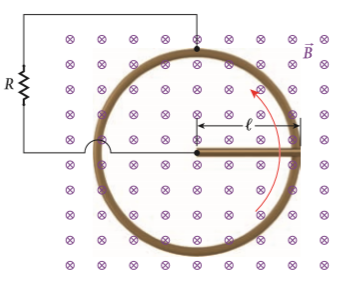
\includegraphics[scale=0.5]{Pictures/rotRod.PNG}
\caption{Problem \ref{rotRod}}
\label{fig:rotRod}
%\addcontentsline{toc}{figure}{Figure \ref{fig:placeholder}} % Uncomment to add the figure to the table of contents
\end{figure}

Figure \ref{fig:rotRod}와 같이 길이 $l$인 도체 막대가 $\omega$의 각속도로 반시계방향으로 회전하고 있고, 종이면 안으로 들어가는 방향으로 자기장이 있다. 이때 저항($R$)의 일률을 구하여라. (Bauer)

\end{problem}



\begin{problem}\label{2014-2(5)}
\begin{figure}[h]
\centering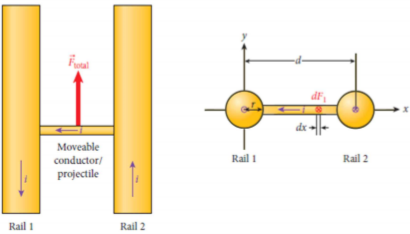
\includegraphics[scale=0.8]{Pictures/2014-2(5).PNG}
\caption{Problem \ref{2014-2(5)}}
\label{fig:2014-2(5)}
%\addcontentsline{toc}{figure}{Figure \ref{fig:placeholder}} % Uncomment to add the figure to the table of contents
\end{figure}
레일건에서 전류는 평행한 두 도체 레일을 따라 흐른다. 각 레일은 길이가 $L$이고 단면의 반지름이 $r$인 원통 형태이다. 전류는 단면에서 골고루 흐른다. 이때 (1) Movable conductor에 작용하는 알짜힘의 크기를 구하여라.[7점] (2) 레일의 끝을 지날때 Movable conductor가 가지는 운동에너지의 크기를 구하여라.[3점] (3) 자기장은 일을 할 수 없음이 알려져 있다. 그렇다면 Movable conductor가 가지는 운동에너지는 어디에서 온 것인가? Movable conductor가 가속되는 기작을 설명하여라.[5점]
(2014-2 기출)
\end{problem}
\begin{problem}\label{2015-1(6)}
\begin{figure}[h]
\centering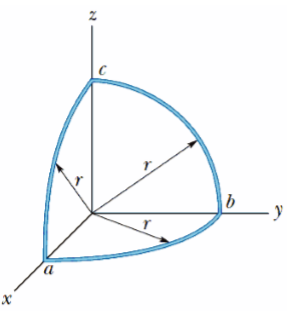
\includegraphics[scale=0.6]{Pictures/2015-1(6).PNG}
\caption{Problem \ref{2015-1(6)}}
\label{fig:2015-1(6)}
%\addcontentsline{toc}{figure}{Figure \ref{fig:placeholder}} % Uncomment to add the figure to the table of contents
\end{figure}
Figure \ref{fig:2015-1(6)}과 같이 반지름이 $r$=10 cm인 원호 3개로 이루어진 고리가 있다. (1) $(1,1,1)$ 방향으로 17.3 mT의 자기장이 작용할 때 이 고리를 통과하는 자속의 크기를 구하여라.[3점] (2) 자기장의 크기가 3.0 mT/s 로 증가할 때 이 고리에 걸리는 기전력의 크기를 구하여라.[2점]  (3) 원호 bc에 걸리는 전류의 방향을 구하여라.[1점] (2015-1 기출)
\end{problem}

\begin{problem}\label{2017-1(4)}
\begin{figure}[h]
\centering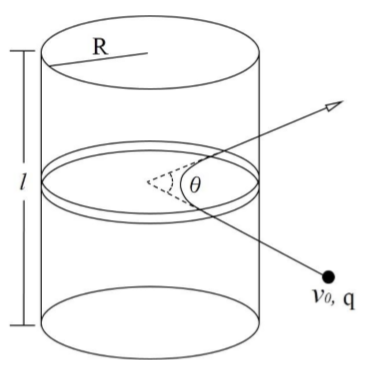
\includegraphics[scale=0.4]{Pictures/2017-1(4).PNG}
\caption{Problem \ref{2017-1(4)}}
\label{fig:2017-1(4)}
%\addcontentsline{toc}{figure}{Figure \ref{fig:placeholder}} % Uncomment to add the figure to the table of contents
\end{figure}
Figure \ref{fig:2017-1(4)}와 같이 가운데에 좁은 틈이 있는 $N$번 감긴 길이 $l$인 솔레노이드가 있다. 이 솔레노이드에 전류 $I$를 흘려 주는 동안, 전하량이 $q$인 입자를 솔레노이드의 중심 방향으로 속도 $v_0$로 발사하였을 때, 
(1) 각 $θ$의 크기를 주어진 문자로 표현하시오. (2) 입자가 솔레노이드 내부를 통과하는 시간 $t_{pass}$를 주어진 문자로 표현하시오. (3) 솔레노이드에 $I_0$의 전류가 흐르고 있을 때, 이 솔레노이드의 인덕턴스 $L$을 구하시오.
(2017-1 기출)
\end{problem}

%----------------------------------------------------------------------------------------
%	CHAPTER 3
%----------------------------------------------------------------------------------------
\chapter{회로이론}
전기회로란 전기 소자가 두 개 이상 연결되어 closed loop를 이루는 것을 말한다. 저항과 축전기, 인덕터를 포함하는 전기회로를 해석하는 방법에 대해서는 물리2에서도 다루었다. 그러나 일반물리학2에서는 더 복잡한 회로를 미분방정식이나 위상자 등의 수학적인 기법을 활용하여 해석하는 방법에 대해 다룬다. 또한, 우리 학교에서는 테브난의 정리와 같이 일반적으로 일반물리학에서 다루지 않는 내용을 배우기도 한다.
일반적으로는 저항을 먼저 다룬 후 축전기와 인덕터에 대해 다루지만, 여기에서는 축전기와 인덕터의 해석을 먼저 다룬 후 비교적 어려운 저항회로의 해석을 다루겠다. 그 다음에는 미분방정식을 이용하여 일반적인 회로를 해석하는 방법을 다루고, 위상자를 이용하여 임피던스를 계산하는 방법을 공부할 것이다.
\section{축전기}
축전기를 직렬/병렬 연결했을 때의 등가 전기용량은 물리2에서 이미 배웠을 것이다.
\begin{remark}
전기용량이 $C_1$, $C_2$인 두 축전기를 연결한 것의 등가 전기용량을 $C$라고 할 때, 축전기를 직렬 연결한 경우 $1/C = 1/C_1 +1/C_2$이고, 축전기를 병렬 연결한 경우 $C=C_1+C_2$이다.
\end{remark}
일반물리학2에서는 이보다 복잡한 상황에서의 등가 전기용량을 구하는 방법을 구하게 된다. 
\begin{example}\label{capacitor2}
Figure \ref{fig:capacitor2} (a)의 회로의 등가 전기용량을 구하여라. 단, 세 축전기의 전기용량은 모두 $C$로 같다. (Irodov)
\end{example}
\begin{figure}[h]
\centering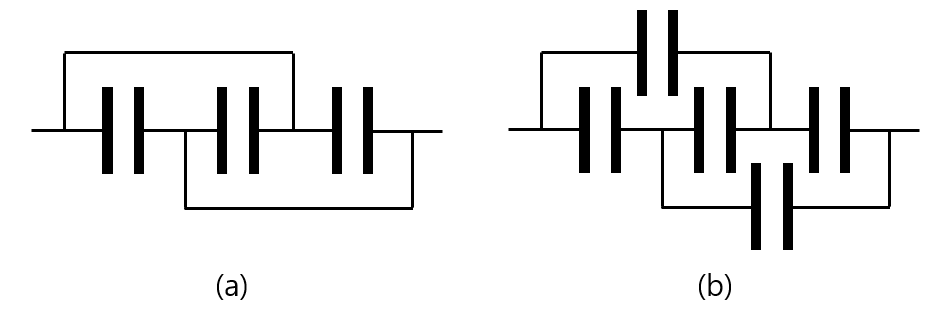
\includegraphics[scale=0.4]{Pictures/capacitor2.PNG}
\caption{Example \ref{capacitor2}}
\label{fig:capacitor2}
%\addcontentsline{toc}{figure}{Figure \ref{fig:placeholder}} % Uncomment to add the figure to the table of contents
\end{figure}
\begin{figure}[h]
\centering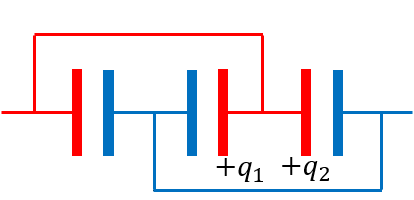
\includegraphics[scale=0.4]{Pictures/capacitor2-1.PNG}
%\addcontentsline{toc}{figure}{Figure \ref{fig:placeholder}} % Uncomment to add the figure to the table of contents
\label{fig:cap2-1}
\caption{Example \ref{capacitor2}}
\end{figure}
회로를 관찰하면 그림과 같이 회로가 두 부분으로 이루어져 있는 것을 알 수 있다. 가운데의 축전기에 $q_1$, 오른쪽 축전기에 $q_2$의 전하가 저장되어있다고 가정한다. 그러면 대칭성에 의해 왼쪽 축전기에 저장된 전하도 $q_2$로 같고, 전체 축전기에 저장된 전하는 $q_1+2q_2$가 된다. 또한 빨간색으로 표시된 곳의 전위는 모두 같은데 첫 번째와 두 번째 축전기에 저장된 전하는 각각 $q_1$과 $q_2$이므로 전위차는 각각 $q_1/C, q_2/C$이다($\because q=CV$). 따라서  $q_1/C-q_2/C=0$이고, $q_1=q_2$이다.\\
따라서 회로 양 끝의 두 지점에서 전위차는 $q_2/C$이다. 전체에 저장된 전하는 $q_1+2q_2=3q_2$이므로, 등가 전기용량은 $C_{eq}=\frac{3q_2}{q_2/C}=3C$이다.
\begin{exercise}
Figure \ref{fig:capacitor2} (b)에 표시된 회로의 등가 전기용량을 구하여라. 단, 모든 축전기의 전기용량은 $C$로 같다. (Irodov)
\end{exercise}
축전기와 관련된 문제를 풀 때는 다음의 사항에 유의하여야 한다.
\begin{enumerate}
\item 충분히 긴 시간이 지난 후라면 축전기는 기본적으로 전기가 통하지 않는 끊겨있는 곳이다. \\이에 따라 위의 예제와 같이 등전위인 부분이 형성되며, 때로는 이러한 부분이 다른 곳과 통하지 않고 고립되어 전하보존을 사용할 수 있기도 한다.반대로, 인덕터는 충분히 긴 시간이 지나면 저항이 없는 도선과 같이 작용한다.
\item 스위치를 닫은 순간에 축전기는 저항이 없는 도선과 같이 작용한다. 반대로 , 인덕터는 스위치를 닫은 순간에는 전류가 흐르지 않는 절연체와 같이 작용한다.
\item 한 축전기의 두 판에 저장된 전하는 크기는 같고 부호가 반대이다.\\이는 가우스 법칙을 사용해 쉽게 보일 수 있다.
\item 축전기에 $V$의 전위차가 걸려 있는 상태로 스위치가 갑자기 열린다면, 축전기는 순간적으로 $V$의 전압을 가진 전지로 작용한다.
\item 전하분포는 항상 전체 계의 에너지가 최소화되는 방향으로 결정된다.
\end{enumerate}
이러한 점에 유의하여 다음 문제를 풀어보자.
\begin{figure}[h]
\centering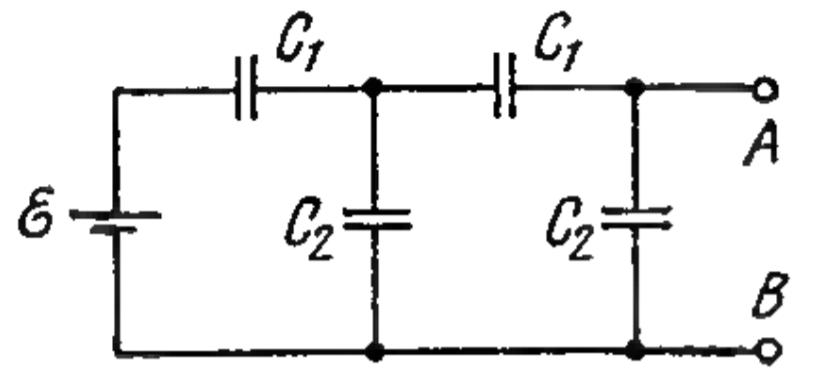
\includegraphics[scale=0.2]{Pictures/capacitor5.PNG}
%\addcontentsline{toc}{figure}{Figure \ref{fig:placeholder}} % Uncomment to add the figure to the table of contents
\caption{Problem \ref{capacitor5}}
\label{fig:capacitor5}
\end{figure}
\begin{exercise}\label{capacitor5}

Figure \ref{fig:capacitor5}와 같은 회로가 있다. $\mathcal{E}=110\mathrm{\;V}$이고 $C_2/C_1=2.0$일 때, A와 B 사이의 전위차를 구하여라. (Irodov)
\end{exercise}

\begin{figure}[h]
\centering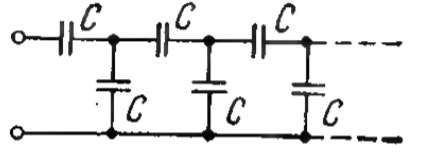
\includegraphics[scale=0.4]{Pictures/capacitor6.PNG}
%\addcontentsline{toc}{figure}{Figure \ref{fig:placeholder}} % Uncomment to add the figure to the table of contents
\caption{Problem \ref{capacitor6}}
\label{fig:capacitor6}
\end{figure}
\begin{exercise}\label{capacitor6}

Figure \ref{fig:capacitor6}와 같이 전기용량이 $C$인 동일한 축전기로 이루어진 무한한 회로가 있다. 이 회로의 등가 전기용량을 구하여라.  (Irodov)
\end{exercise}

\begin{problem}\label{capacitor3}

\begin{figure}[h]
\centering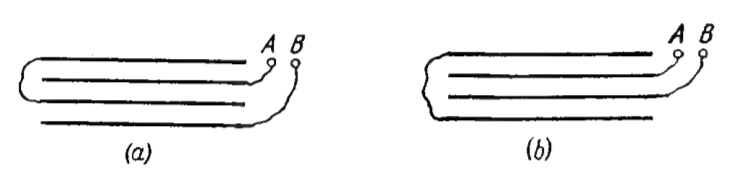
\includegraphics[scale=0.4]{Pictures/capacitor3.PNG}
%\addcontentsline{toc}{figure}{Figure \ref{fig:placeholder}} % Uncomment to add the figure to the table of contents
\label{fig:capacitor3}
\caption{Problem \ref{capacitor3}}

\end{figure}
Figure \ref{fig:capacitor3}와 같이 4개의 동일한 도체 판이 놓여 있고, (a), (b)와 같이 도선으로 연결되어 있다. 각 판의 면적은 $A$이며 판 사이의 간격은 모두 $d$이다. 각 경우에 계의 등가 전기용량을 구하여라. (Irodov)
\end{problem}


\begin{problem}\label{capacitor7}
\begin{figure}[h]
\centering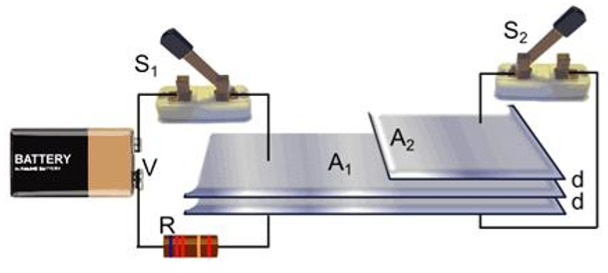
\includegraphics[scale=0.4]{Pictures/capacitor7.PNG}
%\addcontentsline{toc}{figure}{Figure \ref{fig:placeholder}} % Uncomment to add the figure to the table of contents
\caption{Problem \ref{capacitor7}}
\label{fig:capacitor7}
\end{figure}
Figure \ref{fig:capacitor7}과 같이 똑같은 면적 $A_1$을 가지는 두 도체 판이 $d$의 간격을 두고 떨어져있다. 또한 더 작은 면적 $A_2$를 가지는 다른 판이 간격 $d$를 두고 두 도체 판의 위에 배치되어 있다. 처음에 두 스위치 $S_1$과 $S_2$는 열려 있는 상태이다. (1) 스위치 $S_1$을 닫으면 저항에서 얼마만큼의 에너지가 소모되는가?[6점] (2) (1)에서의 과도적 과정이 끝난 후 스위치 $S_2$를 닫으면 얼마만큼의 에너지가 소모되는가?[10점] (2014-2 기출)
\end{problem}

\begin{problem}\label{capacitor8}
\begin{figure}[h]
\centering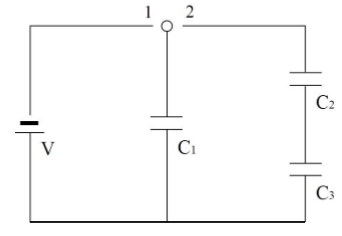
\includegraphics[scale=0.4]{Pictures/capacitor8.PNG}
%\addcontentsline{toc}{figure}{Figure \ref{fig:placeholder}} % Uncomment to add the figure to the table of contents
\caption{Problem \ref{capacitor8}}
\label{fig:capacitor8}
\end{figure}
기전력 V의 전지와 동일한 축전용량을 가지는 축전기 3개를 사용해 Figure \ref{fig:capacitor8}와 같은 회로를 구성하였다. 이때, (1) Switch를 1에 연결하고 시간이 충분히 흘렀다고 할 때 C1에 충전된 에너지를 구하시오. [3점] (2) 이후 Switch를 2에 연결하였다. 이때 각각의 축전기에 저장된 전하량을 구하시오. [4점] (3) (1)에 비하여 (2)에서 손실된 에너지량을 구하시오. [3점] (2017-1 기출)
\end{problem}

\begin{problem}\label{capacitor124}
\begin{figure}[h]
\centering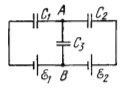
\includegraphics[scale=1.0]{Pictures/3.124.PNG}
%\addcontentsline{toc}{figure}{Figure \ref{fig:placeholder}} % Uncomment to add the figure to the table of contents
\caption{Problem \ref{capacitor124}}
\label{fig:capacitor124}
\end{figure}
Figure \ref{fig:capacitor124}와 같은 상황에서 전위차 $V_A-V_B$를 구하여라. (힌트: 두 축전기 $C_1$과 $C_2$에 대전된 전하량을 각각 $q_1$과 $q_2$라고 놓았을 때 $C_3$에 대전되는 전하량을 생각하라.) (Irodov)
\end{problem}

\begin{problem}\label{capacitor126}
\begin{figure}[h]
\centering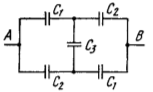
\includegraphics[scale=1.0]{Pictures/3.126.PNG}
%\addcontentsline{toc}{figure}{Figure \ref{fig:placeholder}} % Uncomment to add the figure to the table of contents
\caption{Problem \ref{capacitor126}}
\label{fig:capacitor126}
\end{figure}
Figure \ref{fig:capacitor126}와 같은 회로에서 A 지점과 B 지점 사이의 등가 축전용량을 구하여라. (Irodov)
\end{problem}

\section{전류와 저항}
\paragraph{전류}물리2에서 비저항 $\rho$이고 길이 $L$, 단면적 $A$일 때 저항은 $R=\rho\frac{L}{A}$라고 배웠을 것이다. 그러나 실제 비저항은 전기장과 전류밀도의 비로 정의된다. 즉,
\begin{equation}
\vec{E}=\rho\vec{J}
\end{equation}
이다. 이때 전류밀도는 말 그대로 단면의 단위면적당 흐르는 전류를 의미하며, 방향은 전류의 방향을 가리킨다. 즉, 
\begin{equation}
I=\int \vec{J}\cdot d\vec{a}
\end{equation}
가 성립한다.
비저항의 역수는 전도도라고 하며, $\sigma$로 표시한다. 따라서 $\vec{J}=\sigma\vec{E}$라고 쓸 수 있다. 이러한 비저항과 전도도는 모두 물질의 고유한 특성이다. 비저항은 온도에 따라 변화하는데, 일반적으로 $\rho = \rho_0(1+\alpha (T-T_0))$로 표현된다. \\
전류밀도는 전자의 drift velocity $v_d$와 연관된다. Drift velocity란 전자의 막운동을 고려하지 않은 전자의 평균 이동 속도이다. $dt$만큼의 시간에 전자의 이동 거리는 $v_ddt$이고, 전하밀도를 $n$이라고 하면 $dt$만에 통과하는 전하량 $dq=Aev_dndt$라고 할 수 있다. 따라서
\begin{equation}
i=\frac{dq}{dt}=Aev_dn
\end{equation}
이고, 전류밀도는
\begin{equation}
|\vec{J}|=ev_dn
\end{equation}
이다.

\begin{example}
평행판 축전기의 두 판 사이가 $\rho =100\mathrm{G\Omega\cdot m}$의 비저항을 갖는 유리로 채워져있다. 이 축전기의 축전 용량은 $C=4.0 \mathrm{nF}$이며, 여기에 $V=2.0\mathrm{kV}$의 전압이 걸려 있다. 이때 축전기의 leakage current를 구하여라. (Irodov)
\end{example}

\paragraph{저항회로의 해석}
저항회로를 해석하기 위한 기본이 되는 법칙은 키르히호프 법칙이다.
\begin{theorem}[키르히호프 법칙]\\
\begin{enumerate}
\item 제 1법칙: 전류의 법칙\\회로의 각 노드에서 들어오는 전류의 합과 나가는 전류의 합은 같다.
\item 제 2법칙: 전압의 법칙\\회로 속 닫힌 경로 속에서, 전원의 기전력의 합은 회로 소자의 전압 강하의 합과 같다.
\end{enumerate}
\end{theorem}
지금까지 우리가 회로를 해석하기 위해 사용한 것은 메시해석법으로, 키르히호프 전압 법칙을 사용한 것이다. 일반물리학2에서는 조금 더 복잡한 저항 회로를 해석하는 문제도 출제될 수 있다. 복잡한 저항 회로를 해석할 때에는 등전위인 지점들을 찾는 것이 도움이 된다. 또한, 상황에 따라 등전위인 지점들을 연결하는 전선이 있다고 가정하면 문제를 쉽게 만들 수 있다.
\begin{figure}[h]
\centering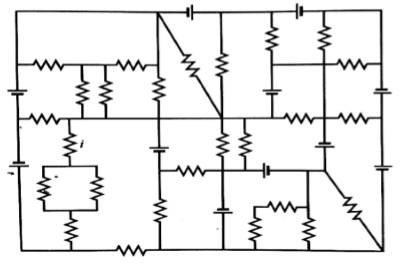
\includegraphics[scale=0.6]{Pictures/capacitor1.PNG}
\caption{Example \ref{capacitor1}}
\label{fig:capacitor1}
%\addcontentsline{toc}{figure}{Figure \ref{fig:placeholder}} % Uncomment to add the figure to the table of contents
\end{figure}
\begin{exercise}\label{capacitor1}
Figure \ref{fig:capacitor1}과 같이 연결된 회로가 있다. 표시된 저항에 흐르는 전류의 크기 $i$를 구하시오. 단, 각 저항의 크기는 모두 4Ω이며 전지의 기전력은 모두 10 V이다. (힌트. 이 문제는 mental calculation을 통해 풀 수 있다.)
(2014-1 기출)
\end{exercise}

\paragraph{노드 해석법}
 지금까지는 회로의 각 메시(mesh)에 대해 키르히호프 전압 법칙을 적용해 회로를 해석하였다. 이와 달리 회로의 각 노드에서 들어오고 나오는 전류의 총 합은 0과 같다는 키르히호프 전류법칙을 이용하여 회로를 해석하는 방법이 있는데, 이를 노드 해석법이라고 한다.
\begin{example}
\begin{figure}[h]
\centering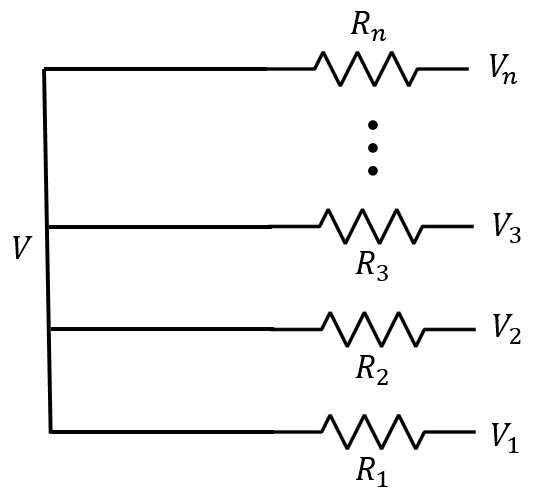
\includegraphics[scale=0.3]{Pictures/node.PNG}
\caption{노드 해석법}
\label{fig:node}
%\addcontentsline{toc}{figure}{Figure \ref{fig:placeholder}} % Uncomment to add the figure to the table of contents
\end{figure}
Figure \ref{fig:node}와 같은 상황에서, 전위 $V$를 구하시오.
\end{example}
위와 같은 경우 맨 왼쪽 노드의 전위를 $V$로 놓을 때, $V_i$로부터 흘러들어오는 전류는 $(V_i-V)/R_i$이다. 따라서 해당 노드에 키르히호프 전류 법칙을 적용하면
\begin{equation}
\frac{V_1-V}{R_1}+\frac{V_2-V}{R_2}+\cdots+\frac{V_n-V}{R_n}=0
\end{equation}
이므로
\begin{equation}
V=\frac{\frac{V_1}{R_1}+\frac{V_2}{R_2}+\cdots+\frac{V_n}{R_n}}{\frac{1}{R_1}+\frac{1}{R_2}+\cdots+\frac{1}{R_n}}
\end{equation}
이 성립하게 된다. 이와 같이 각 노드의 전위를 구하여 회로를 해석하는 방법이 노드 해석법이다.

\begin{exercise}
 기전력의 값이 각각 $\epsilon_1, \epsilon_2$이고 내부저항이 각각 $r_1, r_2$인 두 전지가 있다. 이 두 전지를 병렬로 연결했을 때의 알짜 기전력이
 \begin{equation}
 E_{eq}=\frac{\frac{\epsilon_1}{r_1}+\frac{\epsilon_2}{r_2}}{\frac{1}{r_1}+\frac{1}{r_2}}
 \end{equation}
임을 보이시오. (힌트: 전지가 외부저항 $R$에 연결되어 있는 상황을 가정해보자.) (2014-1 기출)
\end{exercise}
위 예제는 두 전지를 연결한 것의 한쪽 끝의 전위를 0으로 두고 나머지 한쪽 끝에 대해서 노드 해석법을 사용하면 쉽게 해결할 수 있다. 이와 같이 알짜 기전력을 구하는 문제의 경우 외부 저항이 무한대인 상황을 가정하면 된다.


\begin{figure}[h]
\centering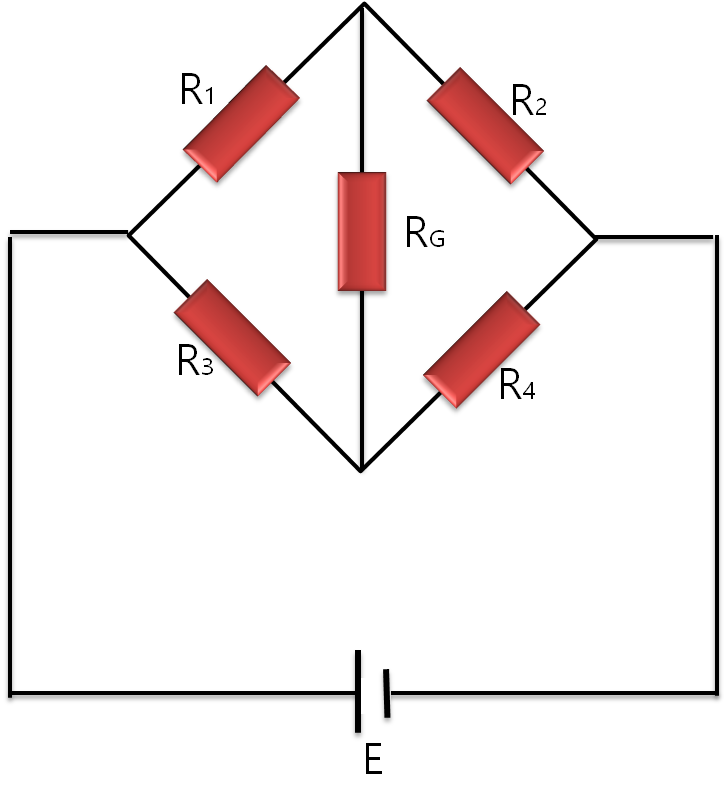
\includegraphics[scale=0.2]{Pictures/wheatstone.png}
\caption{휘트스톤 브리지}
\label{fig:wheatstone}
%\addcontentsline{toc}{figure}{Figure \ref{fig:placeholder}} % Uncomment to add the figure to the table of contents
\end{figure}
\begin{exercise}[휘트스톤 브리지]
Figure \ref{fig:wheatstone}과 같은 회로에서 노드해석법을 사용해 저항 $R_G$에 흐르는 전류의 크기를 구하여라. (힌트: $R_G$의 양 끝에서의 전위를 각각 $V_1$과 $V_2$로 두자.)
\end{exercise}

\paragraph{$Y-\Delta$ 변환}
\begin{example}[$Y-\Delta$ 변환]
\begin{figure}[h]
\centering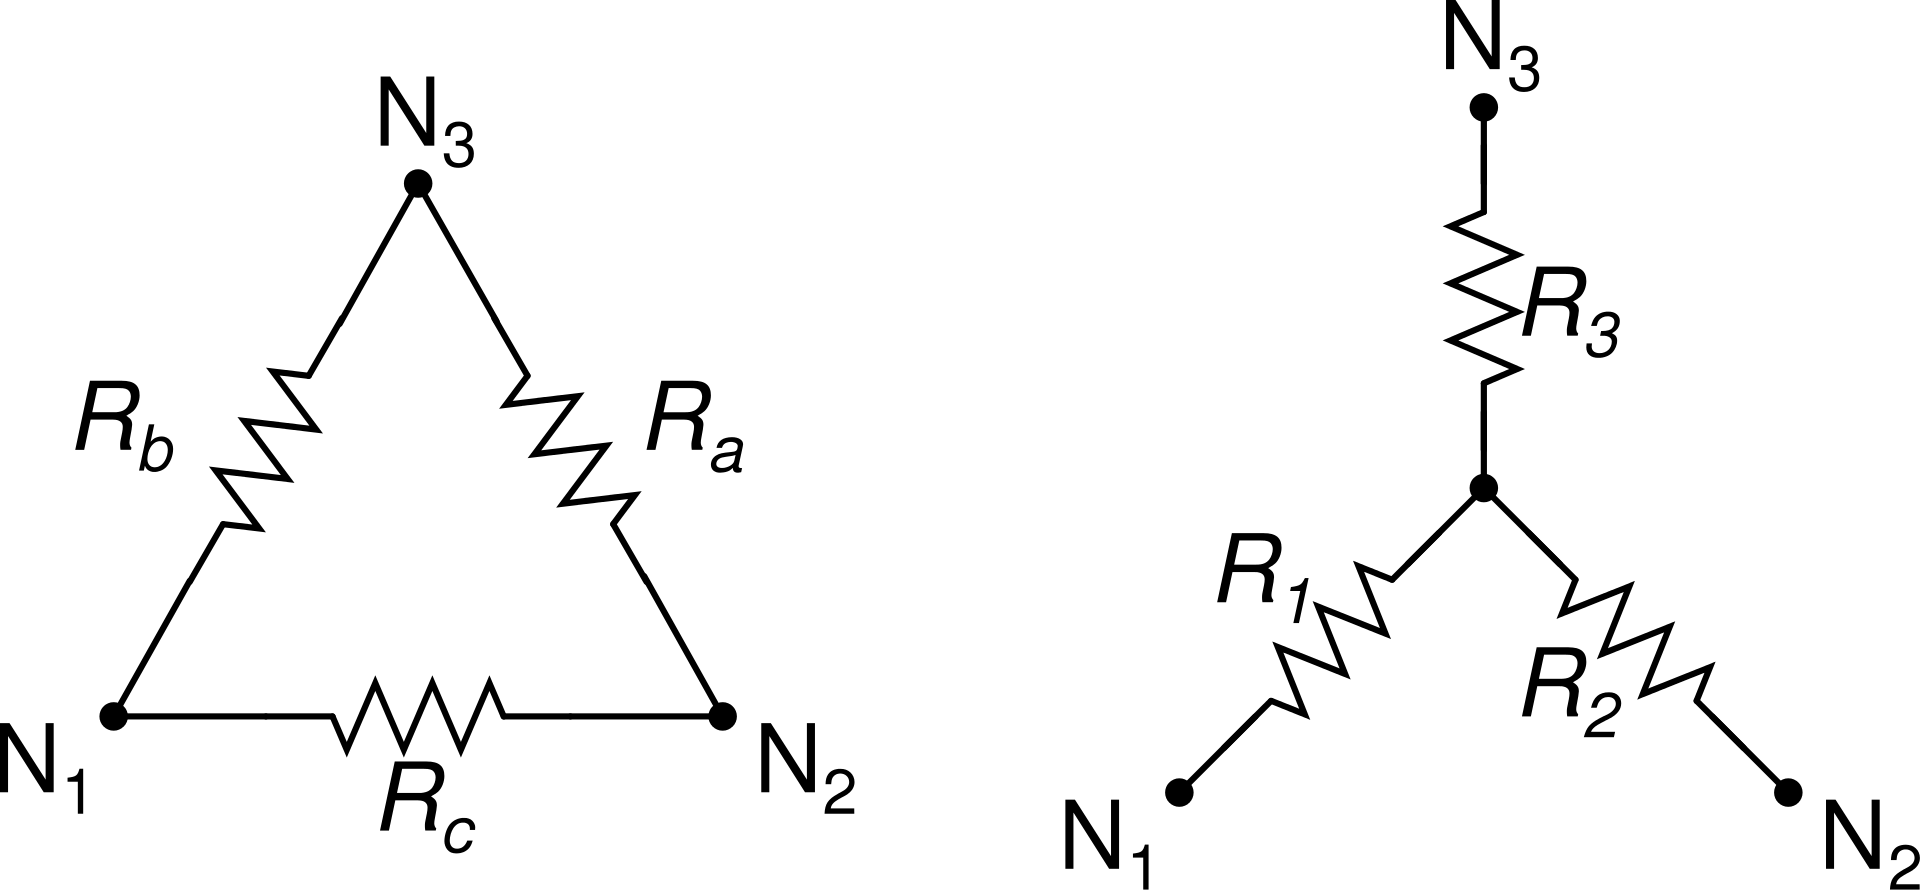
\includegraphics[scale=0.1]{Pictures/y-delta.png}
\caption{$Y-\Delta$  변환}
\label{fig:y-delta}
%\addcontentsline{toc}{figure}{Figure \ref{fig:placeholder}} % Uncomment to add the figure to the table of contents
\end{figure}
Figure \ref{fig:y-delta}의 두 회로가 등가이려면 $R_a, R_b, R_c$와 $R_1, R_2, R_3$의 관계가 어떻게 되어야 하는가?
\end{example}
Figure \ref{fig:y-delta}의 두 회로가 등가라고 함은 세 노드에 어떻게 전압이 걸려도 노드에 흐르는 전류가 두 회로에서 같다는 것이다. 그런데 $N_1$과 $N_2$, $N_2$와 $N_3$, $N_3$와 $N_1$ 사이에 각각 전압을 걸어주었을 때 두 노드 사이에 흐르는 전류가 같아야 하므로, 어떤 두 노드를 잡아도 그 사이의 저항이 같아야 한다고 생각할 수 있다. 따라서
\begin{align}
R_1+R_2 =\frac{1}{1/R_c+1/(R_a+R_b)}\\
R_2+R_3=\frac{1}{1/R_a+1/(R_b+R_c)}\\
R_3+R_1= \frac{1}{1/R_b+1/(R_a+R_c)}
\end{align}
가 성립한다. 연립하면 
\begin{align}
R_1=\frac{R_bR_c}{R_a+R_b+R_c}\\
R_2=\frac{R_aR_c}{R_a+R_b+R_c}\\
R_3=\frac{R_aR_b}{R_a+R_b+R_c}
\end{align}
가 성립함을 알 수 있다.

\begin{exercise}
Figure \ref{fig:wheatstone}과 같은 회로에서 $Y-\Delta$ 변환을 적용해 등가저항을 구하여라.
\end{exercise}

\paragraph{중첩의 원리}
전류밀도와 전기장은 $E=\rho J$의 관계를 가지며, 전류는 $J$를 면에 대해 적분한 것이다. 그런데 전기장은 중첩이 가능하므로 전류밀도 또한 중첩의 원리가 성립함을 알 수 있다. 이를 이용해 문제를 풀 수 있다. 
\begin{exercise}\label{resistor153}
금속 도선이 무한 평면에 정사각형 격자 형태로 배치되어 있으며, 각 변의 저항은 $R$이다. 이때 격자 상에서 이웃한 두 지점 사이의 등가 저항을 구하여라. (힌트: 중첩의 원리를 생각하여라.) (Irodov)
\end{exercise}

\begin{figure}[h]
\centering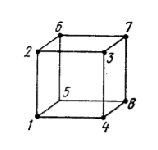
\includegraphics[scale=1.5]{Pictures/3.150.eps}
\caption{Example \ref{resistor150}}
\label{fig:resistor150}
%\addcontentsline{toc}{figure}{Figure \ref{fig:placeholder}} % Uncomment to add the figure to the table of contents
\end{figure}


\begin{problem}\label{resistor150}
Figure \ref{fig:resistor150}와 같이 각각 $R$의 저항을 가지는 와이어가 정육면체 모양을 이루고 있다. (1) 1과 7 사이 (2) 1과 3 사이의 등가 저항을 계산하여라. (3) 또한 1과 3 사이에 $V$의 전위차가 걸렸을 때, 1과 6 사이의 전위차를 구하여라. (Irodov, 2014-2 기출)
\end{problem}

\begin{problem}\label{node5.7}
\begin{figure}[h]
\centering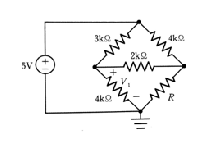
\includegraphics[scale=1.5]{Pictures/node5.7.eps}
\caption{Problem \ref{node5.7}}
\label{fig:node5.7}
%\addcontentsline{toc}{figure}{Figure \ref{fig:placeholder}} % Uncomment to add the figure to the table of contents
\end{figure}
Figure \ref{fig:node5.7}과 같은 회로에서 $V_1=2\mathrm{V}$일 때, $R$의 값을 구하여라. (13년 국가직 7급)
\end{problem}

\begin{problem}\label{node5.8}
\begin{figure}[h]
\centering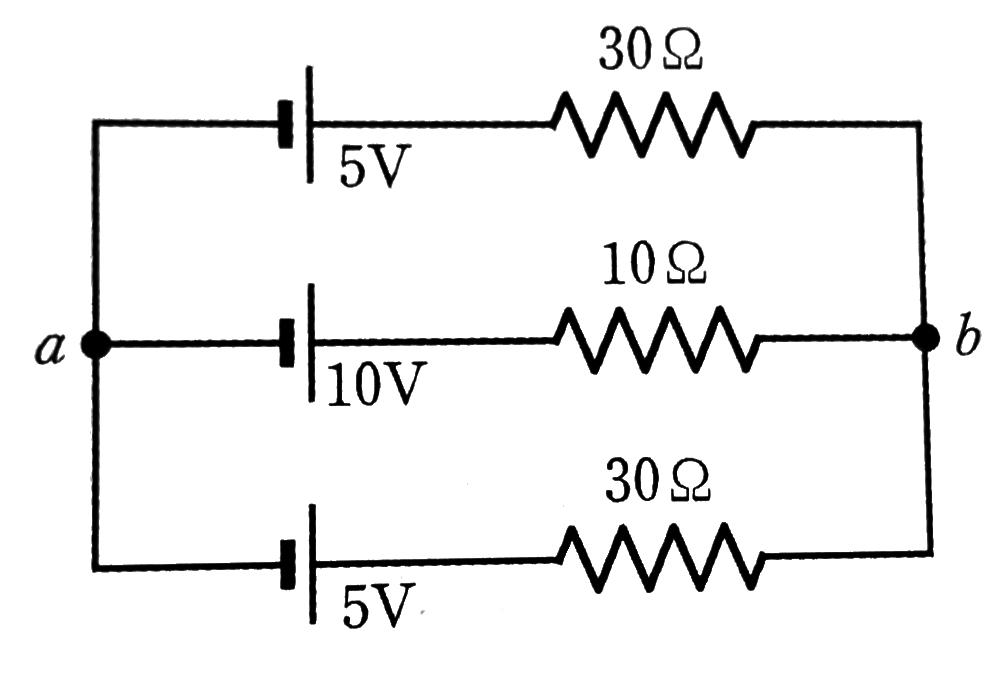
\includegraphics[scale=1.0]{Pictures/node5.8.png}
\caption{Problem \ref{node5.8}}
\label{fig:node5.8}
%\addcontentsline{toc}{figure}{Figure \ref{fig:placeholder}} % Uncomment to add the figure to the table of contents
\end{figure}
Figure \ref{fig:node5.8}과 같은 회로에서 a와 b 사이의 전위차 $V$를 구하여라. (13년 제1회 전기기사)
\end{problem}

\section{일반적인 직류 회로의 해석}
일반물리학2에서는 축전기와 인덕터, 저항이 섞여 있는 일반적인 직류 회로를 미분방정식을 통해 해석하는 방법을 배운다. 저항으로만 이루어진 회로에서와 마찬가지로 임의의 폐곡선을 따라 키르히호프 전압 법칙을 적용하되, $q$에 대한 식으로 나타내면 된다. 이때 저항에서는 $Rdq/dt$, 인덕터에서는 $Ld^2 q/dt^2$, 축전기에서는 $q/C$의 전압 강하가 일어남을 생각하면 된다. 그 후 미분방정식을 풀면 시간에 따른 전하와 전류 등을 알아낼 수 있다.
또한, 스위치를 닫은 직후나 무한히 긴 시간이 지난 후에 관한 문제에서는 다음을 생각하면 된다.
\begin{remark}
충분히 긴 시간이 지난 후라면 축전기는 기본적으로 전기가 통하지 않는 끊겨있는 곳이다. 반대로, 인덕터는 충분히 긴 시간이지나면 저항이 없는 도선과 같이 작용한다.\\
스위치를 닫은 순간에 축전기는 저항이 없는 도선과 같이 작용한다.반대로 , 인덕터는 스위치를 닫은 순간에는 전류가 흐르지 않는 절연체와 같이 작용한다.\\
축전기에 $V$의 전위차가 걸려 있는 상태로 스위치가 갑자기 열린다면, 축전기는 순간적으로 $V$의 전압을 가진 전지로 작용한다.
\end{remark}
\begin{example}[RC 회로]
$V$의 직류 전원에 $R$의 저항을 가진 저항과 $C$의 축전용량을 가진 축전기가 직렬로 연결되어 있다. $t=0$에서 스위치를 갑자기 닫았을 때, 시간에 따라 축전기에 저장된 전하량을 구하여라.
\end{example}
미분방정식을 세우면
\begin{equation}
V=R\frac{dq}{dt}+\frac{q}{C}
\end{equation}
를 얻을 수 있다. 간단한 1계 선형 미분방정식이므로 풀면 
\begin{equation}
q(t) = CV +Ke^{-t/RC}
\end{equation}
를 얻을 수 있다. $q(0)=0$이므로 초기조건을 맞추면
\begin{equation}
q(t)=CV(1-e^{-t/RC})
\end{equation}
를 얻을 수 있다. 여기에서 $\tau=RC$를 시간 상수(time constant)라고 한다.


\begin{example}\label{G7.31}
\begin{figure}[h]
\centering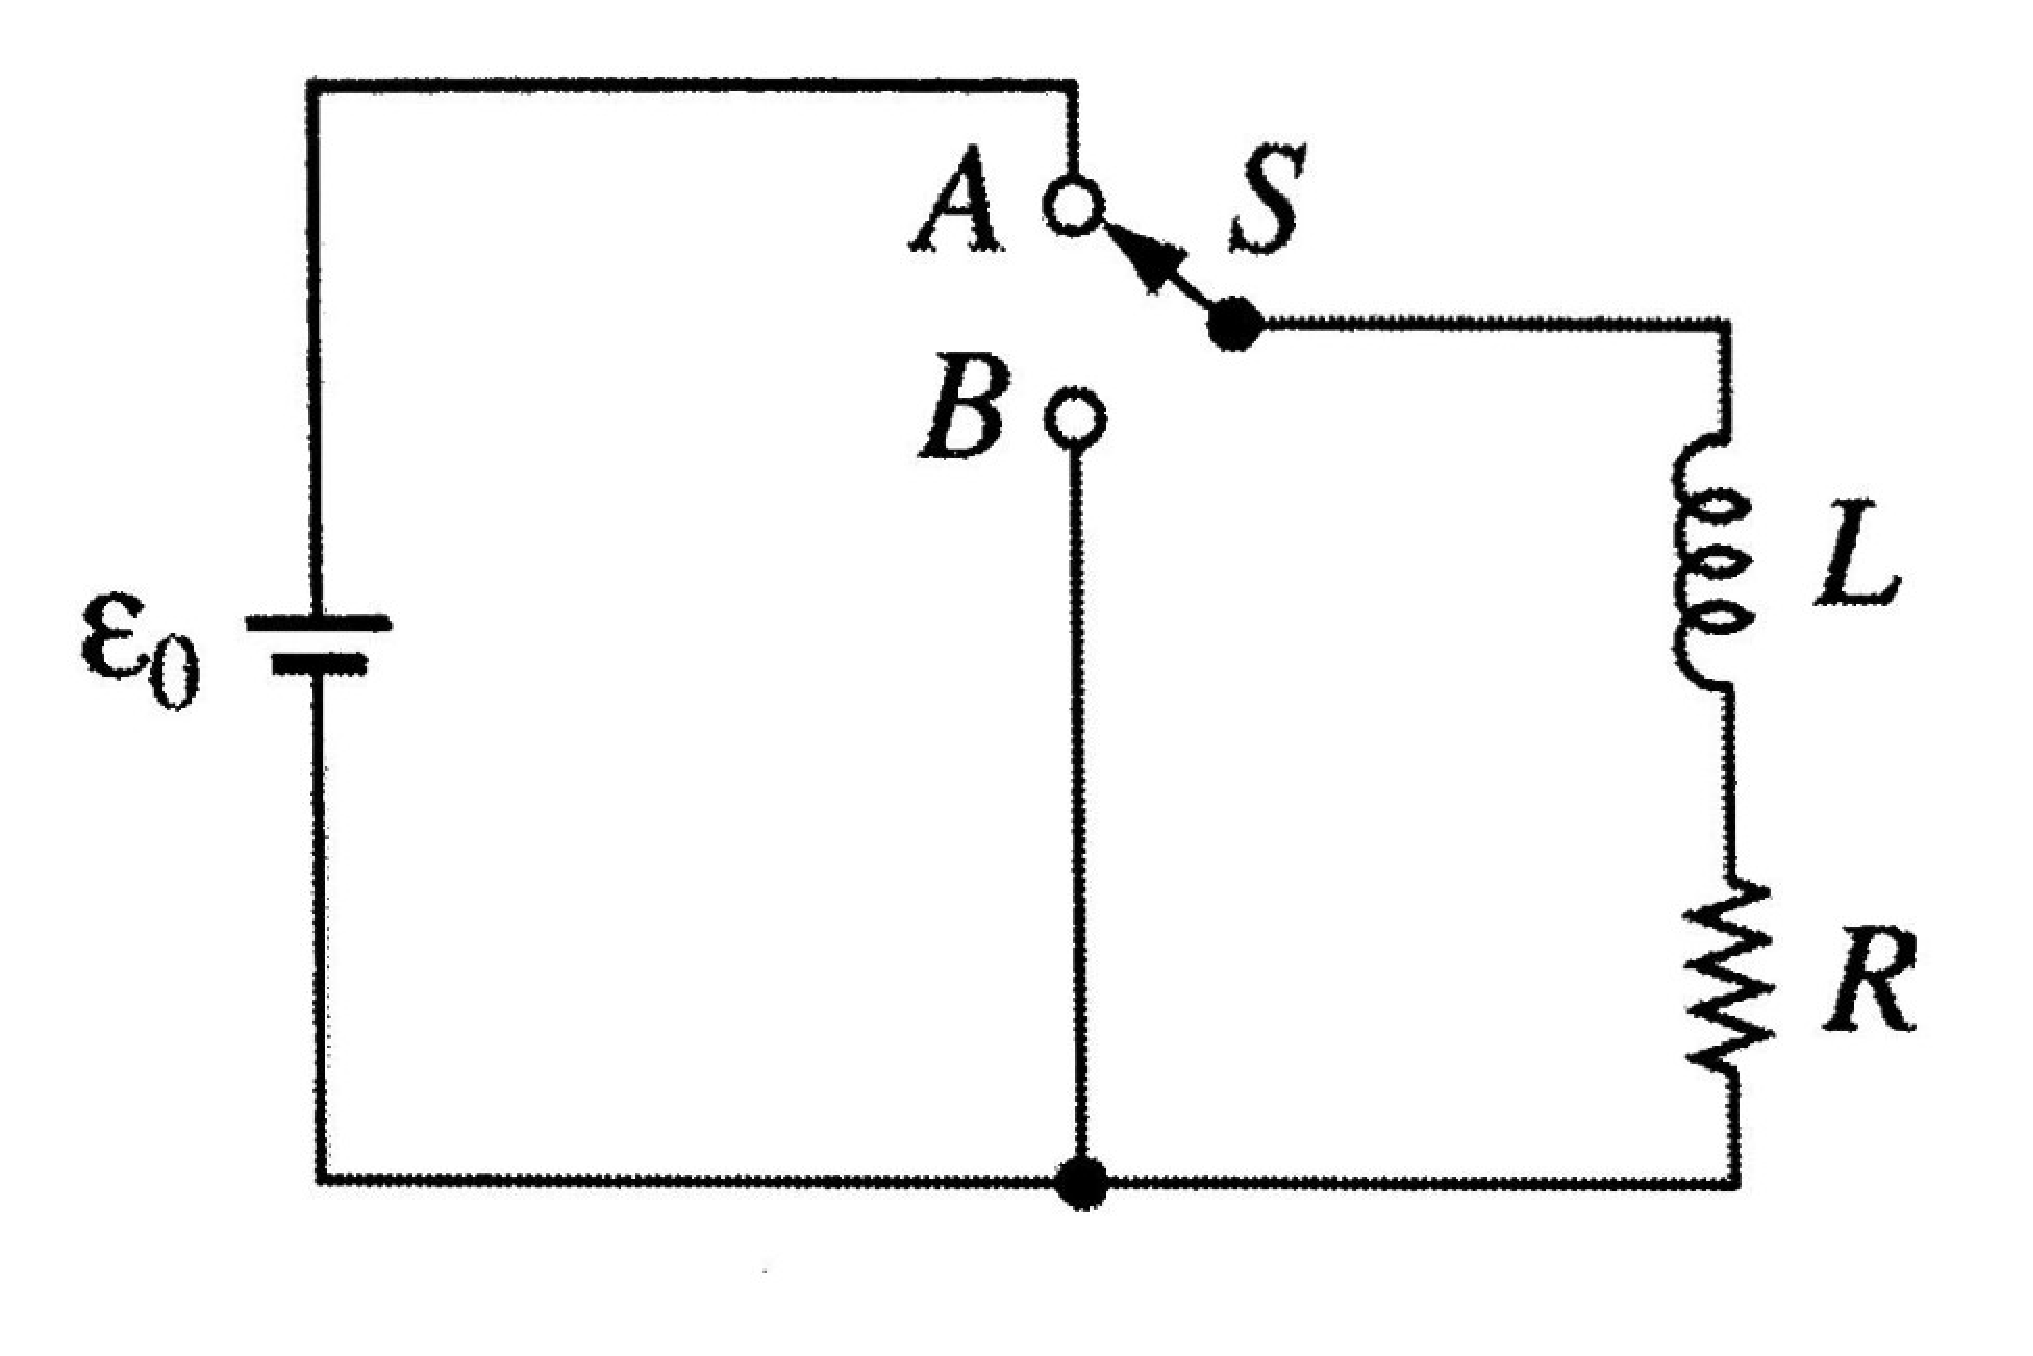
\includegraphics[scale=0.1]{Pictures/G7.31.eps}
\caption{Example \ref{G7.31}}
\label{fig:G7.31}
%\addcontentsline{toc}{figure}{Figure \ref{fig:placeholder}} % Uncomment to add the figure to the table of contents
\end{figure}
Figure \ref{fig:G7.31}의 회로가 오랫동안 전지에 이어져 있다가 한 순간 $t=0$에 스위치 $S$를 갑자기 $A$에서 $B$로 내려 전지가 회로에서 떨어졌다.
(1) 그 뒤 시각 $t$의 전류는 얼마인가? (2) 저항에 전달되는 총 에너지는 얼마인가? (3) 이 에너지는 원래 인덕터에 저장되었던 것과 같음을 밝혀라. (Griffiths)
\end{example}
\begin{exercise}
위의 예제에서 스위치를 갑자기 열었을 때 시간에 따른 축전기에 저장된 전하량을 구하여라.
\end{exercise}

 고리(loop)가 여러 개 있는 회로에서는 그 개수만큼 방정식을 세워 연립하면 된다.
\begin{figure}[h]
\centering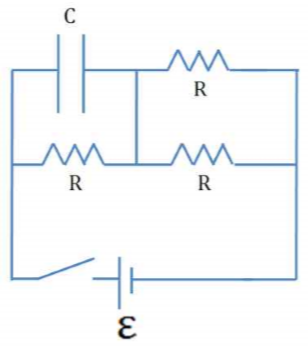
\includegraphics[scale=0.5]{Pictures/2014-2(6).png}
\caption{Exercise \ref{2014-2(6)}}
\label{fig:2014-2(6)}
%\addcontentsline{toc}{figure}{Figure \ref{fig:placeholder}} % Uncomment to add the figure to the table of contents
\end{figure} 
\begin{exercise}\label{2014-2(6)}
 Figure \ref{fig:2014-2(6)}과 같은 회로에서 $R=1.50\mathrm{\Omega}, C=3.50\mathrm{C/V}, \epsilon=3.50\mathrm{V}$이다. $t=0$일 때 스위치는 닫혀 있다고 한다. 이때 (1)축전기에 저장된 전하량 $q(t)$를 구하고, 최대로 충전되었을 때의 전하량을 구하여라. (2) 축전기가 절반만큼 충전될 때까지 걸리는 시간을 구하여라.
 (2014-2 기출)
 \end{exercise}

\begin{problem}\label{2014-2(3)}
\begin{figure}[h]
\centering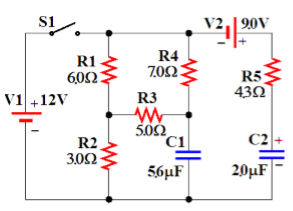
\includegraphics[scale=0.9]{Pictures/2014-2(3).png}
\caption{Problem \ref{2014-2(3)}}
\label{fig:2014-2(3)}
%\addcontentsline{toc}{figure}{Figure \ref{fig:placeholder}} % Uncomment to add the figure to the table of contents
\end{figure}
Figure \ref{fig:2014-2(3)}과 같은 회로가 있다. 이때
(1) 처음에 $S_1$이 열려 있을 때, 각 축전기에 저장된 전하를 구하여라. (2) $S_1$을 닫았을 때, 그 순간에 각 축전기에 흐르는 전류를 구하여라. 그 상태에서 충분히 긴 시간이 흐른 후, (3) $R_4$에 흐르는 전류 (4) 각 축전기에 저장된 전하 (5) $R_3$에서 소모되는 일률을 구하여라. (2014-2 기출)
\end{problem}

\begin{problem}\label{2017-1(3)}
\begin{figure}[h]
\centering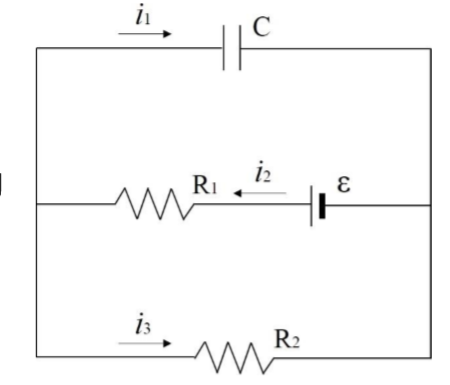
\includegraphics[scale=0.4]{Pictures/2017-1(3).png}
\caption{Problem \ref{2017-1(3)}}
\label{fig:2017-1(3)}
%\addcontentsline{toc}{figure}{Figure \ref{fig:placeholder}} % Uncomment to add the figure to the table of contents
\end{figure}
Figure \ref{fig:2017-1(3)}과 같은 회로에서,
(1) $i_1, i_2, i_3$를 구하기 위한 방정식들을 세우시오. (2) 초기에 $R_1$과 $\epsilon_1$ 사이가 끊어져 있다가 연결되었다. 이때 $C$에 저장되는 $q_1(t)$를 구하시오. (3) (2)와 같은 조건 하에 $i_2(t)$를 구하시오.
(2017-1 기출)
\end{problem}
\begin{problem}\label{2017-1(7)}
\begin{figure}[h]
\centering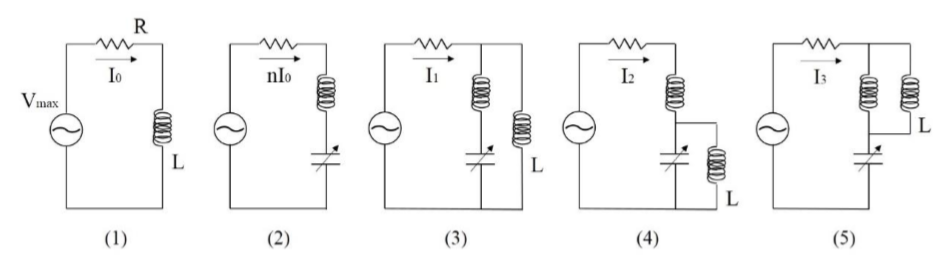
\includegraphics[scale=0.7]{Pictures/2017-1(7).png}
\caption{Problem \ref{2017-1(7)}}
\label{fig:2017-1(7)}
%\addcontentsline{toc}{figure}{Figure \ref{fig:placeholder}} % Uncomment to add the figure to the table of contents
\end{figure}
Figure \ref{fig:2017-1(7)}에서 그림 (1)과 같이 최대전압 $V_{max}$, 저항 $R$, 인덕턴스 $L$의 솔레노이드로 이루어진 회로가 있다. 이 회로에 흐르고 있는 전류의 최대값은 I0였다. 이후 그림 (2)와 같이 가변 축전기를 연결하여 저항 R에 흐르는 전류의 값이 최대가 되도록 해주었다고 할 때 그 전류는 $nI_0$로 나타났다. 이때, 그림 (3), (4), (5)와 같이 회로에 같은 인덕턴스 L을 갖는 솔레노이드를 연결했다면, 각각의 회로의 저항에 흐르는 전류의 최대값 (1) $I_1$ (5 points), (2) $I_2$ (5 points), (3) $I_3$ (5 points) 를 구하여라. 
(2017-1 기출)
\end{problem}
\section{교류 회로의 해석}
이 단원은 물리2에서 배운 교류 회로의 연장선이라 할 수 있는 부분이다.
\begin{remark}
교류회로에서 임피던스(impedance, $Z$)란 전압의 진폭을 전류의 진폭으로 나눈 값이다. 특히 저항과 유도기, 축전기가 전원에 직렬로 연결된 교류 회로에서 임피던스는 $Z=\sqrt{R^2+(X_L-X_C)^2}$의 값을 갖는다.
\end{remark}


\paragraph{감쇠진동}
Figure \ref{fig:damped}와 같은 RLC회로에서 키르히호프 전압법칙을 적용하면 
\begin{figure}[h]
\centering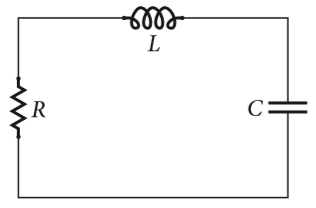
\includegraphics[scale=0.6]{Pictures/damped.PNG}
\caption{RLC 회로}
\label{fig:damped}
\end{figure}
\begin{equation}
L\frac{dq^2}{dt^2}+R\frac{dq}{dt}+\frac{q}{C}=0\label{eq:RLC}
\end{equation}
의 미분방정식을 얻을 수 있다. 이는 $2\omega_\gamma=\frac{R}{L}, \omega_0^2=\frac{1}{LC}$에 대해서
\begin{equation}
\frac{dq^2}{dt^2}+2\omega_\gamma \frac{dq}{dt}+\omega_0^2q=0
\end{equation}
으로 나타낼 수 있다. $q(t)=Qe^{i\omega t}$를 대입하면
\begin{equation}
\omega^2 -2i\omega_\gamma \omega -\omega_0^2=0
\end{equation}
을 얻을 수 있다. 따라서, 
\begin{equation}
\omega_{1,2}=i\omega_\gamma\pm \sqrt{\omega_0^2 -\omega_\gamma^2}
\end{equation}
이다. $\omega_\gamma$와 $\omega_0$의 대소관계에 따라서 이는 3가지로 나뉠 수 있다.
\begin{enumerate}
\item small damping: $\omega_\gamma<\omega_0$\\
이 경우 $\omega_{1,2}=i\omega_\gamma\pm \sqrt{\omega_0^2-\omega_\gamma^2}$이다. 따라서
\begin{align}
q(t)&=Qe^{i(i\omega_\gamma\pm \sqrt{\omega_0^2-\omega_\gamma^2})t}\\
			&= Qe^{-\omega_\gamma t}e^{\pm i\sqrt{\omega_0^2-\omega_\gamma^2}t}
\end{align}이다. 오일러의 공식에 의해 $e^{i\phi}=\cos{\phi}+i\sin{\phi}$이므로
	$Qe^{-\omega_\gamma t}\sin(\sqrt{\omega_0^2-\omega_\gamma^2}t)$와 $Qe^{-\omega_\gamma t}\cos(\sqrt{\omega_0^2-\omega_\gamma^2}t)$가 모두 주어진 미분방정식의 해인데, 식 \ref{eq:RLC}은 선형이므로 중첩의 원리가 적용된다. 따라서 
	\begin{equation}
	    Qe^{-\omega_\gamma t}\cos(\sqrt{\omega_0^2-\omega_\gamma^2}t+\phi)
	\end{equation}
가 이 미분방정식의 	일반해이다. 즉, 축전기에 저장된 전하는 아래 그림과 같이 나타난다.
\begin{figure}[h]
\centering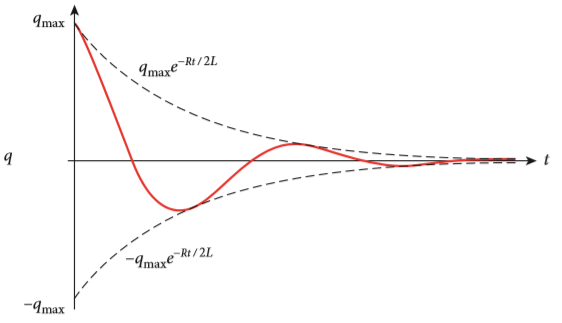
\includegraphics[scale=0.5]{Pictures/small_damping.PNG}
\caption{Small damping}
\label{fig:small_damping}
\end{figure}
\item critical damping: $\omega_0=\omega_\gamma$\\
이 경우 미분방정식의 해는 $Q_1e^{-\omega_\gamma t}$와 $ Q_2te^{-\omega_\gamma t}$이다. 중첩의 원리에 의해서
\begin{equation}
    q(t) = Q_1e^{-\omega_\gamma t}+Q_2te^{-\omega_\gamma t}
\end{equation}
가 일반해이다. 이 경우 진동하는 부분이 없으므로 진동하지 않는다.
\item large damping: $\omega_\gamma>\omega_0$\\
Large damping의 경우에는 
\begin{equation}
    Qe^{(-\omega_\gamma \pm \sqrt{\omega_\gamma^2-\omega_0^2})t}
\end{equation}
가 방정식의 해이다. $-\omega_\gamma \pm \sqrt{\omega_\gamma^2-\omega_0^2}$은 모두 음수이므로, 둘 다 지수적으로 감소한다.
따라서 일반항
\begin{equation}
    q(t)=Q_1e^{(-\omega_\gamma + \sqrt{\omega_\gamma^2-\omega_0^2})t}+Q_2e^{(-\omega_\gamma - \sqrt{\omega_\gamma^2-\omega_0^2})t}
\end{equation}
는 진동하지 않고 지수적으로 감소한다.
\end{enumerate}

\paragraph{강제진동}
\begin{figure}[h]
\centering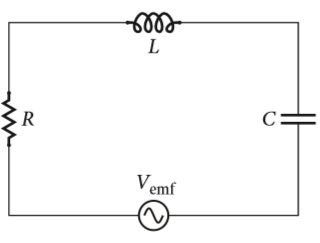
\includegraphics[scale=0.5]{Pictures/driven_RLC.PNG}
\caption{RLC 회로의 강제진동}
\label{fig:driven_RLC}
%\addcontentsline{toc}{figure}{Figure \ref{fig:placeholder}} % Uncomment to add the figure to the table of contents
\end{figure}
Figure \ref{fig:driven_RLC}와 같이 연결된 회로에서, 전원이 $V_{emf}=V_0\sin\omega t$와 같이 주어질 때 미분방정식은
\begin{equation}
L\frac{dq^2}{dt^2}+R\frac{dq}{dt}+\frac{q}{C}=V_0\sin\omega t\label{eq:driven_RLC}
\end{equation}
로 쓸 수 있다. 우변이 0이 아닌 이러한 미분방정식을 비제차(nonhomogeneous)라고 하는데, 이 경우 방정식의 해는 대응되는 제차(homogeneous) 미분방정식
 \begin{equation}
L\frac{dq^2}{dt^2}+R\frac{dq}{dt}+\frac{q}{C}=0
\end{equation}
의 해와 식 \ref{eq:driven_RLC}의 특수해의 합으로 구성된다. 먼저 특수해로 $A\sin\omega t+B\cos\omega t$를 식 \ref{eq:driven_RLC}에 대입하면
\begin{equation}
L(-A\omega^2\sin\omega t - B\omega^2 \cos\omega t)+R(A\omega \cos\omega t - B\omega \sin\omega t)+\frac{1}{C}(A\sin\omega t+B\cos\omega t)=V_0\sin\omega t
\end{equation}
를 얻을 수 있다. 즉,
\begin{equation}
\begin{pmatrix}
-L\omega^2+1/C  & -R\omega\\
R\omega &-L\omega^2+1/C\\
\end{pmatrix}
\begin{pmatrix}
A\\
B\\
\end{pmatrix}
=\begin{pmatrix}
V_0\\
0
\end{pmatrix}
\end{equation}
이므로
\begin{align}
\begin{pmatrix}
A\\
B\\
\end{pmatrix}
&=
\frac{1}{(1/C-L\omega^2)^2+R^2\omega^2}
\begin{pmatrix}
-L\omega^2+1/C  & R\omega\\
-R\omega &-L\omega^2+1/C\\
\end{pmatrix}
\begin{pmatrix}
V_0\\
0
\end{pmatrix}\\
&=
\frac{1}{(1/C-L\omega^2)^2+R^2\omega^2}
\begin{pmatrix}
V_0(1/C-L\omega^2)\\
-RV_0\omega
\end{pmatrix}
\end{align}
이다. 따라서 삼각함수의 합성에 의해 방정식 \ref{eq:driven_RLC}의 특수해는
\begin{equation}
q_p(t)=-\frac{V_0}{\sqrt{(1/C-L\omega^2)^2+R^2\omega^2}}\cos(\omega t-\phi)\quad\quad \phi = \tan^{-1}(\frac{\omega L-\frac{1}{\omega C}}{R})
\end{equation}
이다. 여기에 동차 방정식의 해
\begin{equation}
 Qe^{-\omega_\gamma t}\cos(\sqrt{\omega_0^2-\omega_\gamma^2}t+\phi')
\end{equation}
을 더한
\begin{equation}
q(t)=-\frac{V_0}{\sqrt{(1/C-L\omega^2)^2+R^2\omega^2}}\cos(\omega t-\phi)+ Qe^{-\omega_\gamma t}\cos(\sqrt{\omega_0^2-\omega_\gamma^2}t+\phi')
\end{equation}
이 방정식 \ref{eq:driven_RLC}의 일반해이다. 둘째 항은 진폭이 지수적으로 감소하므로 시간이 지나면 결국 사라지게 되고, 이를 과도해(transient solution)라고 한다. 이후 첫째 항의 특수해만이 남게 된다.

\begin{figure}[h]
\centering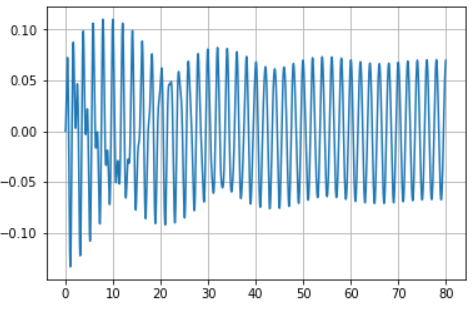
\includegraphics[scale=0.6]{Pictures/forced_oscillation.PNG}
\caption{강제진동의 해. 시간이 지나면서 과도해가 없어지는 것을 확인할 수 있다.}
\label{fig:forced_oscillation}
%\addcontentsline{toc}{figure}{Figure \ref{fig:placeholder}} % Uncomment to add the figure to the table of contents
\end{figure}

\begin{equation}
q(t) = -\frac{V_0}{\sqrt{(1/C-L\omega^2)^2+R^2\omega^2}}\cos(\omega t-\phi)\quad\quad t\gg 0
\end{equation}


따라서 전류는
\begin{align}
i(t) &= \frac{V_0\omega}{\sqrt{(1/C-L\omega^2)^2+R^2\omega^2}}\sin(\omega t-\phi)\\
&= \frac{V_0}{\sqrt{(1/\omega C -L\omega)^2+R^2}}\sin(\omega t-\phi)
\end{align}
와 같이 나타낸다. 따라서 임피던스(엄밀히 말해서는 임피던스의 크기)는 
\begin{equation}
Z=\sqrt{(1/\omega C -L\omega)^2+R^2}
\end{equation}
으로 표현할 수 있다. 임피던스가 최소가 되기 위해서는 위의 식에서 괄호 안에 둘러싸인 부분이 0이 되어야 한다. 따라서
\begin{equation}
1/\omega_0C-L\omega_0=0
\end{equation}
이므로 $\omega_0=\frac{1}{\sqrt{LC}}$를 얻을 수 있다. 이것이 이 계의 공진 각진동수(resonant angular frequency)이다.
\begin{exercise}
RLC 직렬 회로에서 $R=2.20\Omega, L=9.30\mathrm{mH}, C=2.27\mathrm{mF}, V_m=110\mathrm{V}, \omega = 377\mathrm{rad/s}$이다. \\
(1) 전류의 진폭 $I_m$을 구하여라. (2) 위상각 $\phi$를 구하여라. (3) 축전용량 $C$를 조절할 수 있을 때 전류의 진폭이 최대가 되기 위한 $C$의 값을 구하고, 이 때의 전류의 진폭 $I_m$과 위상각 $\phi$를 구하여라.
\end{exercise}

\paragraph{복소 임피던스를 이용한 교류 회로 해석}
일반물리학2에서 작년 기준으로 이시카예프 선생님의 분반에서만 배웠던 복소 임피던스를 이용하면 더 복잡한 회로에서의 임피던스도 쉽게 구할 수 있다. 위상자를 이용해 임피던스를 계산할 때는 유도 리액턴스는 $X_L = j\omega L$로, 용량 리액턴스는 $X_C=1/j\omega C$로 둔다.(정확하게 말하면 임피던스의 허수부를 리액턴스라고 부르는 것이므로, 이는 임피던스라고 불러야 한다.) 이때 $j$는 허수단위로, 전류를 나타내는 $i$와의 중복을 막기 위한 것이다. 이를 저항과 같이 생각하여 등가저항을 계산하듯이 계산하면 복소수 꼴로 계의 임피던스를 계산할 수 있다. 일반물리학의 수준에서는 이 임피던스의 절대값을 임피던스라고 하면 된다. 또한, $\tilde{V}=\tilde{I}\tilde{Z}$이므로 복소수 임피던스의 위상각은 전압과 전류의 위상차와 같다.
다음 예제를 보자.

\begin{example}\label{phasor2}
\begin{figure}[h]
\centering\includegraphics[scale=0.2]{Pictures/phasor2.jpg}
\caption{Example \ref{phasor2}}
\label{fig:phasor2}
%\addcontentsline{toc}{figure}{Figure \ref{fig:placeholder}} % Uncomment to add the figure to the table of contents
\end{figure}
Figure \ref{fig:phasor2}와 같은 RL 병렬회로의 합성 임피던스는?(단, $\omega$[rad/s]는 이 회로의 각 주파수이다.) (14년 2회 전기산업기사 기출)
\end{example}
위상자를 사용하면 이러한 문제를 쉽게 해결할 수 있다. 저항의 임피던스는 $R$이고 유도기의 임피던스는 $X_L=j\omega L$이므로 저항을 병렬 연결할 때와 마찬가지로 

\begin{align}
1/Z&=\frac{1}{R}+\frac{1}{j\omega L}\\
&= \frac{R+j\omega L}{j\omega RL}
\end{align}
이다. 따라서 합성 임피던스는 
\begin{align}
Z&=\frac{j\omega RL}{R+j\omega L}\\
&=\frac{j\omega RL}{R+j\omega L}\frac{R-j\omega L}{R-j\omega L}\\
&= \frac{j\omega R^2 L + \omega ^2 RL^2}{R^2+\omega^2L^2}
\end{align}
이며, 여기에 절대값을 취한
\begin{equation}
|Z|=\frac{\omega R L}{\sqrt{ R^2 +\omega ^2 L^2}}
\end{equation}
이 답이 된다. 추가로, 임피던스의 방향각이
\begin{equation}
\phi = \tan^{-1}\frac{R}{\omega L}
\end{equation}
이므로 전압의 위상은 전류보다 $\phi$만큼 앞서게 된다.
\begin{figure}[h]
\centering\includegraphics[scale=0.15]{Pictures/phasor3.jpg}
\caption{Problem \ref{phasor3}}
\label{fig:phasor3}
%\addcontentsline{toc}{figure}{Figure \ref{fig:placeholder}} % Uncomment to add the figure to the table of contents
\end{figure}
\begin{exercise}\label{phasor3}
Figure \ref{fig:phasor3}와 같은 회로의 공진 주파수에서의 임피던스를 구하여라.
(14년 2회 전기산업기사 기출)
\end{exercise}

\paragraph{주파수 필터}
\begin{figure}[h]
\centering\includegraphics[scale=0.8]{Pictures/freqfilter.PNG}
\caption{저주파 대역 통과 필터. (a) RC 버전 (b) RL 버전}
\label{fig:freqfilter}
%\addcontentsline{toc}{figure}{Figure \ref{fig:placeholder}} % Uncomment to add the figure to the table of contents
\end{figure}
주파수 필터란 주파수 대역에 따라서 통과하는 비율을 다르게 한 회로를 말한다. 주파수 필터 또한 복소수 임피던스를 사용하여 쉽게 분석할 수 있다. 
\begin{example}[저주파 대역 통과 필터]
Figure \ref{fig:freqfilter}(a)의 필터에서 $V_{in}=V_m\cos\omega t$로 주어질 때,  $V_{out}$을 구하여라.
\end{example}
기전력의 비율은 $V_{out}$과 접지 사이의 임피던스 $Z_{out}$과  $V_{in}$과 접지 사이의 임피던스 $Z_{in}$의 비율이다. 즉, $V_{out}/V_{in}=Z_{out}/Z_{in}$이므로 
\begin{equation}
\frac{V_{out}}{V_{in}}=\frac{\frac{1}{j\omega C}}{R+\frac{1}{j\omega C}}=\frac{1}{j\omega RC+1}=\frac{1-j\omega RC}{1+\omega^2 R^2 C^2}=\frac{1}{\sqrt{1+\omega^2 R^2C^2}} e^{j\phi}
\end{equation}
이다($\phi=\tan^{-1}(-\omega RC)$). $V_{in}$은 복소수로 $\hat{V}_{in}=V_me^{j\omega t}$와 같이 나타낼 수 있으므로
\begin{equation}
\hat{V}_{out}=\frac{1}{\sqrt{1+\omega^2 R^2C^2}}V_me^{j(\omega t+\phi)}
\end{equation}
가 성립한다. 실수부를 취하면
\begin{equation}
V_{out}=\frac{1}{\sqrt{1+\omega^2 R^2C^2}}V_m\cos(\omega t+\phi)
\end{equation}
를 얻을 수 있다. 따라서 이 필터는 $\omega$가 작으면 입력전원을 잘 통과시키지만, $\omega$가 커지면 출력이 0에 가까워진다. 
\\주파수 필터에서 breakpoint frequency $\omega_B$는 $|V_{out}|/|V_{in}|$이 $1/\sqrt{2}$이 되는 주파수를 말한다. 따라서 위 예제에서는 $\omega_B=\frac{1}{RC}$이다.
\begin{exercise}
Figure \ref{fig:freqfilter}(b)의 필터에서 $V_{in}=V_m\cos\omega t$로 주어질 때,  $V_{out}$을 구하여라. 또, breakpoint frequency를 구하여라.
\end{exercise}

\begin{exercise}
두 개의 고주파 대역 통과 필터(RC버전, RL버전)를 그려라.
\end{exercise}

고주파 대역 통과 필터와 저주파 대역 통과필터를 연결하면 특정 주파수 사이의 입력전원만을 통과시키는 대역 통과 필터(band-pass frequency filter)를 얻을 수 있다.
\begin{figure}[h]
\centering\includegraphics[scale=0.8]{Pictures/band-pass.PNG}
\caption{대역 통과 필터}
\label{fig:band-pass}
%\addcontentsline{toc}{figure}{Figure \ref{fig:placeholder}} % Uncomment to add the figure to the table of contents
\end{figure}


\begin{problem}
Figure \ref{fig:damped}와 같은 회로에서 각 소자가 $R=10\Omega, L=100\mathrm{\mu H}, C=300\mathrm{pF}$의 값을 가지고 있다. 이 때의 진동수를 구하고, 전류의 진폭이 처음의 $1/e$이 될 때까지 걸리는 시간을 구하여라.  
\end{problem}

\begin{problem}\label{circuit9.2}
\begin{figure}[h]
\centering\includegraphics[scale=0.24]{Pictures/circuit9.2.eps}
\caption{Problem \ref{circuit9.2}}
\label{fig:circuit9.2}
%\addcontentsline{toc}{figure}{Figure \ref{fig:placeholder}} % Uncomment to add the figure to the table of contents
\end{figure}
Figure \ref{fig:circuit9.2}의 회로에서 $t=0$일 때 $i_L=4\mathrm{A}, v_c(0)=0\mathrm{V}$일 때, $t>0$에서 시간에 따른 $v_c(t)$의 값을 구하여라. (기초회로이론)
\end{problem}

\begin{problem}\label{phasor1}
\begin{figure}[h]
\centering\includegraphics[scale=0.20]{Pictures/phasor1.jpg}
\caption{Problem \ref{phasor1}}
%\addcontentsline{toc}{figure}{Figure \ref{fig:placeholder}} % Uncomment to add the figure to the table of contents
\end{figure}
실제 사용하는 유도기와 축전기로 구성된 병렬공진 회로에 대해 (1) 공진 주파수 $\omega_0$를 구하여라. (2) 공진 주파수에서의 임피던스를 구하여라.
(04년 41회 변리사 기출 변형)
\end{problem}

\begin{problem}\label{phasor4}
\begin{figure}[h]
\centering\includegraphics[scale=0.15]{Pictures/phasor4.jpg}
\caption{Problem \ref{phasor4}}
\label{fig:phasor4}
%\addcontentsline{toc}{figure}{Figure \ref{fig:placeholder}} % Uncomment to add the figure to the table of contents
\end{figure}
Figure \ref{fig:phasor4}와 같은 회로의 출력전압 $e_o(t)$의 위상은 입력전압 $e_i(t)$의 위상과 비교해 어떻게 되는가? (14년 1회 전기산업기사 기출)
\end{problem}
\begin{figure}[h!]
\centering\includegraphics[scale=0.4]{Pictures/parallel_RLC.PNG}
\caption{Problem \ref{RLC_parallel}}
\label{fig:RLC_parallel}
%\addcontentsline{toc}{figure}{Figure \ref{fig:placeholder}} % Uncomment to add the figure to the table of contents
\end{figure}

\begin{problem}\label{RLC_parallel}

Figure \ref{fig:RLC_parallel}와 같이 축전기, 저항, 인덕터가 병렬로 연결된 회로가 있다. 진동수 $f$와 $V_{rms}$로 외부 전원이 주어질 때, $I_{rms}$를 $V_{rms}, f, L, C, R$을 이용해 나타내어라. (Bauer)
\end{problem}
\begin{figure}[h!]
\centering\includegraphics[scale=0.8]{Pictures/speaker.PNG}
\caption{Problem \ref{speaker}}
\label{fig:speaker}
%\addcontentsline{toc}{figure}{Figure \ref{fig:placeholder}} % Uncomment to add the figure to the table of contents
\end{figure}

\begin{problem}\label{speaker}
Figure \ref{fig:speaker}과 같이 높은 주파수를 내는 ''tweeter'와 낮은 주파수를 내는 'woofer'로 이루어진 스피커가 있다. $C=10.0\mathrm{\mu F}, L=10.0\mathrm{mH}, R=8.00\Omega$일 때, tweeter와 woofer의 출력이 교차되는 crossover frequency를 구하여라. (Bauer)
\end{problem}
%----------------------------------------------------------------------------------------
%	PART
%----------------------------------------------------------------------------------------

\part{기말고사 범위}

%----------------------------------------------------------------------------------------
%	CHAPTER 4
%----------------------------------------------------------------------------------------


\chapter{전자기파}
\section{맥스웰 방정식}
지금까지 우리가 살펴본 전자기학의 방정식들을 모두 모아 보자면 다음과 같다.
\begin{align}
\oint \vec{E}\cdot d\vec{a}&=\frac{q_{in}}{\epsilon_0}\\
\oint \vec{B}\cdot d\vec{a}&=0\\
\oint \vec{E}\cdot d\vec{l}&=-\frac{d\Phi_B}{dt}\\
\oint \vec{B}\cdot d\vec{l}&=\mu_0 i_{enc}\label{eqn:ampere}
\end{align}
이 중 식 \ref{eqn:ampere}은 맥스웰에 의해 다음과 같이 수정되었다.
\begin{equation}
\oint \vec{B}\cdot d\vec{l}=\mu_0\epsilon_0 \frac{d\Phi_E}{dt}+\mu_0 i_{enc}
\end{equation}
이를 맥스웰-앙페르 법칙이라고 한다. 여기서 새로 추가된 항 $\mu_0\epsilon_0 \frac{d\Phi_E}{dt}$는 패러데이 법칙과 유사하지만 단위를 맞추기 위한 $\mu_0\epsilon_0$가 추가되었고 방향이 반대이고, 즉, 유도 자기장의 방향은 오른손 법칙이 결정하는 것의 반대 방향이다. \\
식에서 보면 $\epsilon_0 \frac{d\Phi_E}{dt}$의 단위가 전류와 같다는 것을 알 수 있다. 이를 변위 전류(displacement current)라고 하며, $i_d$로 쓴다. 따라서 맥스웰-앙페르 법칙은 
\begin{equation}
\oint \vec{B}\cdot d\vec{l}=\mu_0(i_{enc}+i_d)
\end{equation}
로 쓸 수 있다. 
\begin{example}[평행판 축전기의 충전]\label{dispcur}
반지름이 $R$인 원통형의 평행판 축전기에 $i$의 전류가 흐르면서 충전되고 있다. 이때 변위전류의 크기를 구하고 축전기의 축에서 반지름 방향으로 $d>R$만큼 떨어진 지점에서의 자기장을 구하여라.
\end{example}
\begin{figure}[h]
\centering\includegraphics[scale=0.4]{Pictures/dispcur.PNG}
\caption{Example \ref{dispcur}}
\label{fig:dispcur}
%\addcontentsline{toc}{figure}{Figure \ref{fig:placeholder}} % Uncomment to add the figure to the table of contents
\end{figure}
$\dfrac{dq}{dt}=i$이고 전기장은 $E=\dfrac{\sigma}{\epsilon_0}=\dfrac{q}{\epsilon_0\pi R^2}$이다. 따라서  
\begin{equation}
i_d=\epsilon_0\frac{d\Phi_E}{dt}=i
\end{equation}
이다. $\oint \vec{B}\cdot d\vec{a}=2\pi d \cdot B=\mu_0 i_d=\mu_0 i$이므로 자기장은 $\dfrac{\mu_0 i \hat{\phi}}{2\pi d}$ 임을 알 수 있다.
위 예제와 같이 변위전류는 실제 전류와 비슷한 성질을 가지기도 한다. 
\begin{exercise}
Example \ref{dispcur}의 상황에서 반지름 방향으로 $d<R$만큼 떨어진 지점에서의 자기장을 구하여라. 또, $d>R$인 경우와 합쳐서 그래프로 나타내어라.
\end{exercise}
이렇게 수정된 맥스웰-앙페르법칙을 비롯하여 네 개의 방정식을 묶어서 맥스웰 방정식이라고 한다.
\begin{align}
\oint \vec{E}\cdot d\vec{a}&=\frac{q_{in}}{\epsilon_0}\\
\oint \vec{B}\cdot d\vec{a}&=0\\
\oint \vec{E}\cdot d\vec{l}&=-\frac{d\Phi_B}{dt}\\
\oint \vec{B}\cdot d\vec{l}&=\mu_0\epsilon_0 \frac{d\Phi_E}{dt}+\mu_0 i_{enc}
\end{align}
이는 적분형으로, 스토크스 정리와 발산 정리를 사용하여 미분형으로 고칠 수도 있다.
\begin{theorem}[스토크스 정리]
폐곡선 $\partial R$에서 수행되는 선적분은 다음과 같이 폐곡선이 둘러싸는 영역인 $R$에서의 면적분으로 변환될 수 있다.
\begin{equation}
\oint_{\partial R} \vec{F}\cdot d\vec{l}=\iint_R (\nabla \times \vec{F}) \cdot d\vec{a}
\end{equation}
\end{theorem}
\begin{theorem}[발산 정리]
폐곡면 $\partial R$에서 수행되는 면적분은 다음과 같이 폐곡면이 둘러싸는 영역인 $R$에서의 공간적분으로 변환될 수 있다.
\begin{equation}
\oint_{\partial R} \vec{F}\cdot d\vec{a}=\iiint _R (\nabla \cdot \vec{F}) d\tau
\end{equation}
\end{theorem}
이를 통해 미분형으로 고친 맥스웰 방정식은 다음과 같다.
\begin{align}
&\nabla \cdot \vec{E}=\frac{\rho}{\epsilon_0}\\
&\nabla \cdot \vec{B}=0\\
&\nabla \times \vec{E}=-\frac{\partial \vec{B}}{\partial t}\\
&\nabla \times \vec{B}=\epsilon_0\mu_0\frac{\partial \vec{E}}{\partial t}+\mu_0 \vec{J}\\
\end{align}
\section{전자기파}
맥스웰 방정식에서 전하도, 전류도 없는 진공 상태를 생각하자. 그러면 아래와 같은 식이 만들어진다.
\begin{align}
&\nabla \cdot \vec{E}=0\\
&\nabla \cdot \vec{B}=0\\
&\nabla \times \vec{E}=-\frac{\partial \vec{B}}{\partial t}\label{eq:faraday}\\
&\nabla \times \vec{B}=\epsilon_0\mu_0\frac{\partial \vec{E}}{\partial t}\\
\end{align}
식 \ref{eq:faraday}의 좌변에 $\nabla \times$를 취해주면 다음과 같다. 
\begin{equation}
\nabla \times \nabla \times \vec{E}=\nabla (\nabla \cdot \vec{E})-\nabla^2 \vec{E}
\end{equation}
그런데, $\nabla \cdot \vec{E}=0$이므로 
\begin{align}
-\nabla ^2 \vec{E}&=\nabla \times \left( -\frac{\partial \vec{B}}{\partial t}\right)\\
&= -\frac{\partial}{\partial t}\nabla \times \vec{B}\\
&= -\frac{\partial}{\partial t}\epsilon_0\mu_0\frac{\partial \vec{E}}{\partial t}\\
&= -\epsilon_0\mu_0 \frac{\partial ^2 \vec{E}}{\partial t^2}
\end{align}
이고,
\begin{equation}
\nabla ^2 \vec{E}=\epsilon_0\mu_0 \frac{\partial^2\vec{E}}{\partial t^2}
\end{equation}
이 성립한다. 마찬가지로 
\begin{equation}
\nabla ^2 \vec{B}=\epsilon_0\mu_0 \frac{\partial ^2 \vec{B}}{\partial t^2}
\end{equation}
도 성립한다. 이는 일차원에서의 파동방정식인 
\begin{equation}
\frac{\partial ^2 f}{\partial s^2}-\frac{1}{v^2}\frac{\partial ^2 f}{dt^2}=0
\end{equation}
을 3차원으로 옮긴 것으로, 똑같이 파동방정식에 해당하며 진행속도는 $c=\dfrac{1}{\sqrt{\epsilon_0\mu_0}}=299792458\mathrm{m/s}$이다.
\begin{figure}[h]
\centering\includegraphics[scale=0.6]{Pictures/em.PNG}
\caption{전자기파의 진행}
%\addcontentsline{toc}{figure}{Figure \ref{fig:placeholder}} % Uncomment to add the figure to the table of contents
\end{figure}
\paragraph{포인팅 벡터}
전자기파의 에너지 수송률은 다음과 같이 표현할 수 있다.
\begin{equation}
\vec{S}=\frac{1}{\mu_0}\vec{E}\times\vec{B}
\end{equation}
이를 포인팅 벡터(Poynting vector)라고 한다. $|\vec{S}|$는 전자기파의 세기(intensity)로, 전자기파에 의해 수송되는 에너지의 단위면적당 일률을 의미한다.  이는 전자기파에만 적용되는 것은 아니고, 임의의 전자기장에 적용이 가능하다.

\begin{exercise}
반지름 $r$, 길이 $L$이고 저항이 $R$인 도체에 $V$의 전압이 걸려 있다. 이에 따라서 $i$의 전류가 흐르며 바깥에 $B$의 자기장을 만들고 있다. 도체가 $y$축을 따라 놓여 있으며 전류가 $+y$ 방향으로 흐르고 있으며 전기장은 도체 전체에서 균일하다고 가정할 때, (1) 표면에서 포인팅 벡터의 크기와 방향을 구하여라. (2) $\oint \vec{S}\cdot d\vec{a}=i^2R$임을 보여라. (Bauer)
\end{exercise}


그런데 전자기파는 진동하므로 $E=E_0\cos(ks-\omega t), B=B_0\cos(ks-\omega t)$로 쓸 수 있고, 전기장과 자기장은 항상 수직하므로 특정 순간의 전자기파의 세기는 
\begin{equation}
S=\frac{1}{\mu_0}EB\cos^2(ks-\omega t)
\end{equation}
이다. 그런데
\begin{equation}\label{eq:eblight}
E/B=c
\end{equation}
이고, 주기 $T=2\pi/\omega$에 대해
\begin{equation}
\frac{1}{T}\int_0^{T} \cos^2(ks-\omega t)dt=1/2
\end{equation}
이므로 전자기파의 평균 세기는
\begin{align}
S_{avg}&=\left ( \frac{1}{\mu_0}EB\cos^2(ks-\omega t)\right )_{avg}\\
&= \frac{1}{2\mu_0 c}E^2 \label{eq:intensity}
\end{align}
임을 알 수 있다. 일반적으로 이것을 그냥 전자기파의 세기라고 한다.\\
포인팅 벡터는 전자기파가 아닌 임의의 전자기장이 존재할 때도 적용될 수 있다. 그러나 전자기파가 아닌 경우에는 식 \ref{eq:eblight}이 적용되지 않으므로 식 \ref{eq:intensity}와 같은 식은 사용할 수 없음에 유의하여야 한다. 
\paragraph{전자기장의 운동량과 압력}
\begin{theorem}[전자기파의 운동량]
평면파 형태의 전자기파가 $\Delta t$만큼의 시간동안 완전히 흡수되었으며 그 에너지의 크기가 $\Delta U$라면,그 에너지 표면으로 흡수되는 운동량의 크기는
\begin{equation}\label{eq:emmomentum}
\Delta p = \Delta U /c
\end{equation}
이다.
\end{theorem}
정확하게 말하자면 전자기파뿐만 아니라 일반적인 전자기장에도 운동량이 있으며, 그 밀도는 $\vec{g}=\epsilon_0 \vec{E}\times \vec{B}=\mu_0\epsilon_0 \vec{S}=\frac{1}{c^2}\vec{S}$이다.\\
또한 힘은
\begin{equation}
F=\frac{\Delta p}{\Delta t}=\frac{\Delta U}{c\Delta t}=\frac{IA\Delta t}{c\Delta t}
\end{equation}
이므로, 전자기파에 의한 압력은
\begin{equation}\label{eq:empressure}
p_r=\frac{I}{c}
\end{equation}
이다. 이때 $I$는 전자기파의 세기(intensity)이다. 만약 전자기파가 완전히 흡수되는 대신에 완전히 반사된다면, 식 \ref{eq:emmomentum}과 \ref{eq:empressure}에 각각 2를 곱해주면 된다.

\begin{exercise}
$1.00\mathrm{mW}$의 일률을 가진 초록색 레이저가 있다. 이 레이저를 거울의 $2.00\mathrm{mm}$의 지름을 갖는 원 모양의 영역에 비추었을 때, 레이저 포인터가 거울에 작용하는 힘의 크기를 구하여라. (Bauer)
\end{exercise}

\begin{problem}
반지름이 $R$이고 두꼐가 $d$인 원통형 축전기가 있다. 이 축전기에 $V$의 전압이 걸려 있으며 $i$의 전류가 흐르면서 충전되고 있다. 이때 축전기 옆면에서의 포인팅 벡터의 크기와 방향을 구하고, $\oint \vec{S}\cdot d\vec{a}$를 구하여라.
\end{problem}

\begin{problem}
1.00 mm의 지름을 가지는 Continuous-wave(CW) 아르곤 레이저가 10.0W의 평균 일률로 발사되고 있다. 빔의 세기가 단면 전체에서 일정하다고 가정할 때, (1) 레이저 빔의 세기를 구하고 지구 표면에서의 태양광 세기인 1400 W/m\textsuperscript{2}와 비교하여라. (2) 전기장의 rms 세기를 구하여라. (3) 포인팅 벡터의 평균값을 구하여라. (4) 빔의 파장이 514.5 nm일 때 특정 순간의 포인팅 벡터를 $t$와 $x$에 대해 표현하여라. 단, $t=0, x=0$일 때 포인팅 벡터는 0이다. (5) 자기장의 rms 세기를 구하여라. (Bauer) 
\end{problem}
\begin{problem}
\begin{equation}
\vec{E}=E_0\cos(\alpha x+2\alpha y-\omega t)\hat{z}
\end{equation}
일 때,
(1)$T=0$일 때, phase가 $0, 2\pi, 4\pi, 6\pi$의 wavefront를 구하여라.
(2)	$\omega$를 $\alpha$로 표현하여라.
(3)	$\vec{B}$를 구하여라.
(4)	포인팅 벡터를 구하여라.(2019-2 기출)
\end{problem}


%----------------------------------------------------------------------------------------
%	CHAPTER 5
%----------------------------------------------------------------------------------------
\chapter{파동광학}
\section{간섭}
$d$의 간격을 두고 떨어져 있는 $N$개의 슬릿을 생각하자. 각 슬릿은 두께가 없다. 
\begin{figure}[h]
\centering\includegraphics[scale=0.6]{interference.PNG}
\caption{간섭}
\label{fig:interference} % Unique label used for referencing the figure in-text
%\addcontentsline{toc}{figure}{Figure \ref{fig:placeholder}} % Uncomment to add the figure to the table of contents
\end{figure}
각 슬릿을 통해 빛이 들어온다고 할 때, 빛은 전자기파이므로 위에서 $n$번째 슬릿의 전기장을 근사하여
\begin{equation}
E_0\cos(k(r_1+(n-1)d\sin\theta)-\omega t)
\end{equation}라고 쓸 수 있다. 이때 $\theta$는 슬릿이 있는 평면의 법선에 대한 각도이다. 오일러의 공식에 의해서 임의의 각 $\theta$에 대해
$e^{i\theta} = \cos\theta +i\sin\theta$가 성립하므로 이를 
\begin{equation}
E_0e^{k(r_1+(n-1)d\sin\theta)-\omega t}
\end{equation}
라고 쓰고, 나중에 실수부만 취하기로 하자. 그러면 총 전기장은
\begin{equation}
\tilde{E_{net}}=E_0e^{i(kr_1-\omega t)} (1+e^{ikd\sin\theta}+e^{2ikd\sin\theta}+\cdots +e^{(N-1)ikd\sin\theta})
\end{equation}
로 쓸 수 있다. 
\begin{equation}
A=1+e^{ikd\sin\theta}+e^{2ikd\sin\theta}+\cdots +e^{(N-1)ikd\sin\theta}=\frac{1-e^{iNkd\sin\theta}}{1-e^{ikd\sin\theta}}
\end{equation}
라고 할 때, 
\begin{align}
&|A|^2=AA^* \\
&=\frac{1-e^{iNkd\sin\theta}}{1-e^{ikd\sin\theta}}\frac{1-e^{-iNkd\sin\theta}}{1-e^{-ikd\sin\theta}} \\
&=\frac{2-(e^{-Nikd\sin\theta} +e^{Nikd\sin\theta})}{2-(e^{-ikd\sin\theta}+e^{ikd\sin\theta})} \\
&= \frac{2-2\cos(Nkd\sin\theta)}{2-2\cos(kd\sin\theta)}\\
&=\left(\frac{\sin(Nkd\sin\theta/2))}{\sin(kd\sin\theta/2)}\right )^2
\end{align}
이 성립한다.  따라서 $\delta = kd\sin\theta$라고 할 때, 스크린의 한 점 상에서 빛의 세기는
\begin{align}
I&=\left(\frac{1}{\mu_0c}E_{net}^2\right)_{avg}\\
&=\left(\frac{1}{\mu_0c}  E_0 \cos^2 (kr_1-\omega t) \frac{\sin^2(N\delta/2)}{\sin^2(\delta/2)}
\right)_{avg}\\
&=\frac{1}{2\mu_0c}  E_0 \frac{\sin^2(N\delta/2)}{\sin^2(\delta/2)}\\
&=I_0 \frac{\sin^2(N\delta/2)}{\sin^2(\delta/2)}\label{eq:multslit}
\end{align}
가 된다. 이 때 $I_0$는 간섭과 같은 효과를 무시할 때 하나의 슬릿에서 나오는 빛의 세기이다. 식 \ref{eq:multslit}은 분모가 0이 될 때 최대가 되며, 분자가 0이 될 때 최소가 된다. 이때 분모가 0이 되더라도 $\sin(\delta/2)=0$이라면 $\sin(N\delta/2)$ 또한 0이 되기 때문에 발산하지 않으며, $N^2$으로 수렴한다. 
이를 그래프로 나타내면 다음과 같다.
\begin{figure}[!htb]
\minipage{0.32\textwidth}
  \includegraphics[width=\linewidth]{Pictures/n=2.PNG}
  \caption{$N=2$인 경우 }\label{fig:awesome_image1}
\endminipage\hfill
\minipage{0.32\textwidth}
  \includegraphics[width=\linewidth]{Pictures/n=3.PNG}
  \caption{$N=3$인 경우}\label{fig:awesome_image2}
\endminipage\hfill
\minipage{0.32\textwidth}%
  \includegraphics[width=\linewidth]{Pictures/n=4.PNG}
  \caption{$N=4$인 경우}\label{fig:awesome_image3}
\endminipage
\end{figure}
$N\gg 1$인 경우는 회절격자와 대응된다. 이러한 경우에는 다음과 같은 그래프가 나타나게 된다. 
\begin{figure}[h]
\centering\includegraphics[scale=0.5]{Pictures/n=20.PNG}
\caption{회절 격자의 경우 빛의 세기($N=40$)}
\label{fig:diffgrating}
\end{figure}
\begin{figure}[h]
\centering
\includegraphics[width=0.5\textwidth]{Pictures/5.69.eps}
\caption{Exercise \ref{5.69}}
\label{fig:5.69}
\end{figure}
\begin{exercise}\label{5.69}
Lloyd의 거울 실험(Figure \ref{fig:5.69})에서, 얇은 슬릿 $S$에서 나온 빛이 거울 M에 반사된 빛과 간섭하여 스크린 Sc에 간섭 무늬가 만들어졌다. 광원은 스크린에서 $l = 100 \mathrm{cm}$만큼 떨어져 있다. 광원이 특정 지점에 있을 때 스크린에 맺힌 간섭 무늬의 폭이 $\Delta x=0.25\mathrm{mm}$였으며, 광원을 거울면에서 $\Delta h =0.60\mathrm{mm}$만큼 멀어지게 했을 때 간섭무늬의 폭은  $\eta = 1.5$배만큼 좁아졌다고 한다. 이때 빛의 파장을 구하여라. (Irodov)
\end{exercise}

\begin{problem}
한쪽 면은 볼록하고 반대쪽 면은 평면인 렌즈(plano-convex lens)가 볼록한 면을 아래로 하여 유리판에 맞닿아있다. 볼록한 면의 곡률이 $R$이고, 빛의 파장은 $\lambda$이라고 한다. 이 때 뉴턴 링 사이의 간격 $\Delta r$을 $r$의 함수로 표현하여라. (단, $\Delta r \ll r$이다.) (Irodov)
\end{problem}

\begin{problem}\label{5.71}
\begin{figure}[h]
\centering
\includegraphics[scale=0.5]{Pictures/5.71.eps}
\caption{Problem \ref{5.71}}
\label{fig:5.71}
\end{figure}
Figure \ref{fig:5.71}은 Fresnel mirrors를 이용한 실험을 나타낸다. 두 거울 사이의 각도 $\alpha = 12'$이고, 두 거울의 교선과 슬릿 $S$, $Sc$까지의 거리는 각각 $r=10.0\mathrm{cm}$, $b=130\mathrm{cm}$이다. 빛의 파장이 $\lambda = 0.55\mathrm{pm}$일 때, (1) 스크린에 맺히는 무늬의 폭을 구하여라. (2) 슬릿이 중심이 $O$이고 반지름이 $r$인 원의 접선 방향으로 $\Delta l=1.00\mathrm{mm}$ 움직였을 때, 간섭 무늬는 얼마나 움직이는가? (3) 스크린에 맺히는 간섭 무늬가 충분히 선명하게 보이기 위한 슬릿의 최대 폭 $\delta_{max}$를 구하여라. (Irodov)
\end{problem}

\begin{problem}
두께 $5.0\mathrm{cm}$, 초점거리가 $f=25.0\mathrm{cm}$인 볼록렌즈를 중심을 따라 이등분하여 사이의 두께 $1.00\mathrm{mm}$인 부분을 깎아낸 후 다시 붙여서 합성 렌즈를 만들었다. Focal plane에 얇은 슬릿이 파장 $\lambda = 0.60\mathrm{\mu m}$의 단색광을 내보내고 있으며 렌즈 뒤쪽으로  $b=50\mathrm{cm}$ 떨어진 지점에 스크린이 놓여 있을 때, (1) 스크린에 맺히는 회절 무늬의 개수와 가능한 maxima의 개수 (2) 회절 무늬가 충분히 선명하게 보이기 위한 슬릿의 최대 두께 $\delta_{max}$를 계산하여라. (Irodov)
\end{problem}

\begin{problem}
Fresnel biprism에게서 $a=25\mathrm{cm}$ 떨어진 곳에 얇은 슬릿이, $b=100\mathrm{cm}$ 떨어진 곳에는 스크린이 위치해 있다. Biprism의 굴절각이 $\theta = 20'$이고 스크린에 맺히는 회절 무늬의 폭이 $\Delta x = 0.55\mathrm{mm}$일 때, 슬릿에서 나오는 빛의 파장을 구하여라. (Irodov)
\end{problem}

\begin{problem}
A microwave transmitter at height $h$ above the horizontal reflective surface(Lloyd's mirror) transmits microwaves of wavelength $\lambda$ toward a receiver on the distance $R$, at the same height $h$ above the mirror. The microwaves reflecting from the mirror interfere with the microwave arriving directly from the transmitter. 
(a) Find an expression that gives the values of R for which the signal at the receiver is maximum. (Hint: Does the reflection cause a phase change?)
(b) If the receiver shows a power $P_0$ at distance from the transmitter without the reflective surface, what is a reading if there is the reflector between them? (2017-2 기출)
\end{problem}


\section{회절}
이번에는 $Nd$를 일정하게 두고 $N\to\infty$로 가는 경우를 생각해보자. 이 경우는 빛이 나오는 곳이 무수히 많기 때문에 슬릿의 두께가 있을 경우의 단일 슬릿 회절무늬와 대응된다. 이 경우 슬릿의 폭은 $w=Nd$라고 할 수 있다.
이때
\begin{align}
I&=I_0 \frac{\sin^2 (k/2\cdot Nd\sin\theta)}{\sin^2 (k/2\cdot d\sin\theta)}\\
&=I_0N^2 \frac{\sin^2 (k/2\cdot w\sin\theta)}{N^2\sin^2 (k/2\cdot d\sin\theta)}\\
&\approx I_0N^2 \frac{\sin^2 (k/2\cdot w\sin\theta)}{N^2\sin^2 (k/2\cdot d\sin\theta)} \frac{\sin^2 (k/2\cdot d\sin\theta)}{(k/2\cdot d\sin\theta)^2}\\
&= I_0N^2 \frac{\sin^2 (k/2\cdot w\sin\theta)}{(k/2\cdot w\sin\theta)^2}
\end{align}
따라서 $\beta = \frac{1}{2}kw\sin\theta$라고 하면 빛의 세기는 
\begin{equation}
I=I_0N^2 \frac{\sin^2 \beta}{\beta^2}
\end{equation}
으로 쓸 수 있다. $N$은 더 이상 의미가 없으므로 $I_0N^2$을 새로 $I_0$로 정의하면, 
\begin{equation}
I=I_0 \frac{\sin^2 \beta}{\beta^2}\label{eq:singlediff}
\end{equation}
이다. 이를 그래프로 나타내면 다음과 같다.
\begin{figure}[h]
\centering\includegraphics[scale=0.5]{Pictures/diffraction.PNG}
\caption{단일 슬릿 회절 무늬}
\label{fig:diffslit}
\end{figure}

원형의 구멈을 통한 회절의 경우, first diffraction minimum을 다음과 같이 얻을 수 있다.
\begin{equation}
\sin\theta=1.22\frac{\lambda}{d}
\end{equation}
이때 $\theta$는 구멍의 중심을 지나는 법선과의 각도를 의미한다. 두 천체를 망원경을 통해 관측할 때와 같은 경우, 렌즈를 통해 바라본 두 천체가 구별되기 위한 기준은 하나의 central maximum이 나머지 하나의 first diffraction minimum 안으로 들어가지 않는 것이다. 이를 레일리 기준(Rayleigh's criterion)이라 한다.

\begin{exercise}
허블 우주 망원경의 주반사경은 지름이 $2.4\mathrm{m}$이다. 이때 초록색 빛에 대한 이 망원경의 angular resolution을 구하여라. (Bauer)
\end{exercise}



\paragraph{회절 격자}
회절 격자(diffraction grating)란 슬릿과 같이 빛을 통과시킬 수 있는 구멍이 수백 개 모여 이루어진 것을 말한다. 또한, 구멍 대신 거울으로 이루어진 회절 격자 또한 존재한다. 회절 격자의 성질로는 분산(dispersion)과 분해능(resolving power)이 있다. 먼저 분산이란 $\lambda$에 따라 회절되는 각도가 얼마나 민감하게 변화하는지 나타내는 척도, 즉 $\theta$의 $\lambda$에 대한 변화율을 말한다. $\sin\theta = m\frac{\lambda}{d}$이므로, 이는
\begin{equation}
D=\frac{d\theta}{d\lambda}=\frac{d}{d\lambda}\left ( \sin^{-1}\left ( \frac{m\lambda}{d}\right )\right)=\frac{1}{\sqrt{1-(\frac{m\lambda}{d})}}\frac{m}{d}=\frac{m}{d\cos\theta}
\end{equation}
로 나타낼 수 있다. \\
해상도란 가까이 있는 두 maxima를 떼어 놓는, 즉 분해하는 능력을 뜻하며 이는 각 maximum의 너비에 의존하는 값이다. 두 maxima의 파장을 각각 $\lambda_1, \lambda_2$라고 할 때, 분해 가능한 파장의 가장 작은 차이가 $\Delta\lambda_{min}=\lambda_2-\lambda_1$이라고 하면, 해상도는
\begin{equation}
R=\frac{\lambda_{avg}}{\Delta \lambda_{min}}
\end{equation}
으로 정의된다. 이때 $\lambda_{avg}=\frac{1}{2}(\lambda_1+\lambda_2)$이다. 그런데 두 광선의 회절 각도를 $\theta_1, \theta_2$라고 할 때, $\Delta \theta = \theta_{hw}$일 때 겨우 분리가 가능하다. 또한 $\theta_{hw}$의 각도는 first diffraction minimum과 같으므로, $\sin\theta_{hw}=\frac{\lambda}{a}=\frac{\lambda}{Nd}$이다. 
\begin{figure}[h]
\centering\includegraphics[scale=0.5]{Pictures/resolving_power.png}
\caption{Central maximum의 half-width}
\label{fig:diffslit}
\end{figure}
$\sin\theta_{hw}\approx \theta_{hw}$이므로 $\theta_{hw} = \frac{\lambda}{Nd}$이며, 일련의 과정을 통해 1차가 아닌 다른 차수의 maxima에서 $\theta_{hw} = \frac{\lambda}{Nd\cos\theta}$임을 보일 수 있다. 그런데 $D=\frac{d\theta}{d\lambda}$이므로 $\Delta\lambda=\frac{\Delta \theta}{D}=\lambda/Nm$이다. 따라서
\begin{equation}
R=\frac{\lambda_{avg}}{\Delta \lambda}=Nm
\end{equation}
임을 알 수 있다.
\paragraph{이중 슬릿 간섭}
이중 슬릿의 경우에는 위의 폭이 있는 단일 슬릿 2개가 $d$의 간격을 두고 중첩되어 있는 것이다. 따라서 식 \ref{eq:singlediff}과  \ref{eq:multslit}을 적용하면 각도 $\theta$에 따른 빛의 세기는 다음과 같이 표현할 수 있다. ($\alpha =\frac{1}{2}\delta = \frac{1}{2}kd\sin\theta$)
\begin{align}
I&=I_0 \frac{\sin^2\beta}{\beta^2}\frac{\sin^2(2\alpha)}{\sin^2(\alpha)}\\
&=4I_0 \frac{\sin^2 \beta}{\beta^2}\cos^2\alpha
\end{align}
파동광학 파트에서는 이상의 유도 과정을 모두 외워두는 것이 좋다.
\begin{exercise}
폭이 $w$인 슬릿 3개가 $d$씩 떨어져 있을 때, 이것이 만들어 내는 무늬를 각도에 따른 세기 형태로 나타내시오.
\end{exercise}

\begin{exercise}
$\lambda=0.50\mathrm{\mu m}$의 파장을 가진 빛이 $b=10\mathrm{\mu m}$의 폭을 가진 슬릿의 법선과 $30^\circ$의 각도를 이루며 입사하고 있다. 이 때 central Fraunhofer maximum의 양 쪽에 형성되는 first minima의 위치를 각도로 표현하여라. (Irodov)
\end{exercise}

\begin{problem}
$\lambda = 530\mathrm{nm}$의 파장을 가진 빛이 $1.50\mathrm{\mu m}$의 주기를 가진 투명한 회절격자로 입사하고 있다. 입사각이 (1) $0^\circ$일 때와 (2) $60^\circ$일 때, 각각 가장 높은 차수의 Fraunhofer maximum의 각도를 구하여라. (Irodov)
\end{problem}

\begin{problem}
Point source 6개가 나란히 있고, lambda = d/2의 파장으로 빛이 나오고 있다. 이때
(1) 1번째 principal maxima의 각도를 구하여라
(2)$-\pi/2\le\theta\le\pi/2$의 범위 안에 있는 principal maxima의 개수를 구하여라.
(3) 첫번째 dark fringe의 각도를 구하여라.
(4) 파장을 바꾸었을 때, 첫번째 principal maximum 바로 옆의 dark fringe였던 자리에 새로운 first principal maximum이 위치하게 된다. 이때 파장을 구하시오. (2019-2 기출)
\end{problem}


\chapter{상대성 이론}
\section{상대성 이론}
\begin{definition}[관성 좌표계]
관성 좌표계(inertial reference frame)란 외부에서 알짜 힘이 작용할 때에만 물체가 가속되는 좌표계를 뜻한다.
\end{definition}
\begin{theorem}[상대성 이론의 가정]
상대성 이론의 기반이 되는 아인슈타인의 가정은 다음과 같다.\\
\begin{enumerate}
\item 물리 법칙은 모든 관성 좌표계에서 같다.
\item 빛의 속도는 모든 관성 좌표계에서 $c=299792458\mathrm{m/s}$로 일정하다.
\end{enumerate}
\end{theorem}
\begin{definition}[$\beta$ 인자와 $\gamma$ 인자]
물체의 속도가 $\vec{v}$일 때, 
\begin{equation}
\vec{\beta}=\vec{v}/c\quad\quad\gamma=\frac{1}{\sqrt{1-\beta^2}}
\end{equation}
로 정의한다. 1차원에서, $-1\le \beta \le 1$이며 $\gamma\ge 1$이다. 
\end{definition}
특수 상대성 이론의 대표적인 두 현상인 길이 수축과 시간 팽창은 물리2에서 이미 배웠을 것이다.

\begin{remark}
정지한 관측자가 측정하였을 때 같은 장소에서 $\Delta t_0$의 간격으로 벌어진 두 사건은, 이 관측자 기준으로 $v$의 속력으로 움직이는 관측자가 측정할 때에는
\begin{equation}
\Delta t = \gamma \Delta t_0=\frac{1}{\sqrt{1-(v/c)^2}}\Delta t_0
\end{equation}
의 간격으로 측정된다.
\end{remark}
\begin{remark}
정지된 관측자가 측정하였을 때 같은 시간에 $\Delta L_0$의 간격으로 벌어진 두 사건은, 이 관측자 기준으로 $v$의 속력으로 움직이는 관측자가 측정할 때에는
\begin{equation}
\Delta L = \Delta L_0 /\gamma = \sqrt{1-(v/c)^2}\Delta L_0
\end{equation}
의 간격으로 측정된다.
\end{remark}

\begin{theorem}[로런츠 변환]
관성계 $S$의 관측자가 보았을 때 시공간 좌표 $(t, x,y,z)$에서 일어난 사건이 $S$에 대해 속도 $\vec{v}=(v,0,0)$의 속도로 움직이는 관성계 $S'$의 관측자가 보았을 때 $(t',x',y',z')$에서 일어났다면, 이는
\begin{equation}
\begin{pmatrix}
ct'\\
x'\\
y'\\
z'\\
\end{pmatrix}
= \begin{pmatrix}
\gamma& -\gamma\beta& 0& 0\\
-\gamma\beta & \gamma & 0 & 0 \\
0&0&1&0\\
0&0&0&1\\
\end{pmatrix}
\begin{pmatrix}
ct\\
x\\
y\\
z\\
\end{pmatrix}
\end{equation}
의 관계를 갖는다. 이를 로런츠 변환(Lorentz transformation)이라고 한다.
\end{theorem}
어떤 두 사건이 $(\Delta t, \Delta x, \Delta y, \Delta z)$만큼의 차이를 두고 일어난다면, $-c^2(\Delta t)^2 +(\Delta x)^2 + (\Delta y ) ^ 2 + (\Delta z)^2$은 어떤 좌표계에서 관측해도 불변이다. 이를 로런츠 불변량(Lorentz invariant)이라고 한다. 이것이 양수라면 두 사건 사이의 간격(interval)이 '공간같다(spacelike)'고 하며, 음수라면 '시간같다(timelike)'고 한다. 0이라면 '빛같다(lightlike)'고 한다.\\
시간같은 간격에 대해
\begin{equation}
-c^2(\Delta t)^2 +(\Delta x)^2 + (\Delta y ) ^ 2 + (\Delta z)^2=-c^2(\Delta \tau)^2
\end{equation}
인 $\Delta \tau$를 고유시간이라고 하며, 공간같은 간격에 대해
\begin{equation}
-c^2(\Delta t)^2 +(\Delta x)^2 + (\Delta y ) ^ 2 + (\Delta z)^2=(\Delta s)^2
\end{equation}
인 $\Delta s$를 고유길이라고 한다. 즉, 고유시간은 두 사건이 같은 장소에서 발생한 것으로 보이는 관측자가 볼 때의 시간 간격이며 고유길이는 두 사건이 같은 시각에 발생한 것으로 보이는 관측자가 볼 때의 길이이다. 만약 두 사건이 원인과 결과의 관계라면 두 사건은 공간같을 수 없다. 공간같다면 $-c^2(\Delta t)^2 +(\Delta x)^2 >0$이므로 $\Delta x/\Delta t>c$가 되기 때문이다. 정보의 전달 속도는 빛보다 빠를 수 없다.
\begin{example}
어떤 관성계에 대해 정지된 관측자가 볼 때, 두 섬광(flash)이 동시에 발생하였다. 이 관측자가 볼 때 두 섬광이 $\Delta x$의 거리를 두고 발생하였다면, 이 관측자에 대해 $0.25c$의 상대속도로 움직이는 다른 관측자가 볼 때에 두 섬광이 일어난 시간의 차이와 거리를 구하여라. 또,  두 사건이 시간같은지, 공간같은지, 또는 빛같은지 말하여라.
\end{example}
먼저, 첫 번째 관측자가 볼 때 두 섬광이 동시에 발생하였다고 하였으므로 두 사건은 '공간같다'라고 할 수 있다. 또한 $\gamma = 4/\sqrt{15}, \beta = 0.25$이므로 
\begin{equation}
\begin{pmatrix}
ct'\\
x'\\
\end{pmatrix}
= \begin{pmatrix}
4/\sqrt{15}& -1/\sqrt{15}\\
-1/\sqrt{15}&4/\sqrt{15}
\end{pmatrix}
\begin{pmatrix}
0\\ 
\Delta x
\end{pmatrix}
= \begin{pmatrix}
-\Delta x/\sqrt{15}\\
4\Delta x/\sqrt{15}\\
\end{pmatrix}
\end{equation}
따라서, 이 관찰자가 보았을 때 두 사건은 $\Delta t'=-\Delta x/\sqrt{15}c$만큼의 시간과 $\Delta x' = 4\Delta x/\sqrt{15}$의 공간을 두고 떨어져 있는 것으로 보인다.

\paragraph{로런츠 속도 변환}
관성계 $S$에서 관측한 속도를 $v$라고 하고, $S$에 대해 $V$의 속도로 운동하는 $S'$에서 관측한 속도를 $v'$이라고 하자. 그러면 $v'=\frac{dx'}{dt'}$이다. 그런데 $\gamma = \frac{1}{\sqrt{1-(V/c)^2}}$라고 할 때, 로런츠 변환에 의해 $dx=\gamma V dt' + \gamma dx'$이고, $dt=\gamma( dt' +\frac{Vdx}{c^2})$이다. 또한, $v=\frac{dx}{dt}$이므로 $dx=vdt$이다. 따라서, 
\begin{equation}
v'=\frac{dx'}{dt'}=\frac{\gamma(V+v)dt}{\gamma(dt+Vvdt/c^2)}=\frac{v+V}{1+vV/c^2}
\end{equation}
임을 알 수 있다. (여러 속도를 더해야 할 때에는 빠르기(rapidity) $\theta = \tanh^{-1}(v/c)$를 정의하면 $\theta'=\Theta +\theta$가 성립하여 편리하다.)

\begin{exercise}
관성계 $S$에서 $v_y$의 속력으로 $+y$ 방향으로 움직이는 물체가 있을 때, $S$에 대해 $+x$ 방향으로 $V$의 속도로 움직이는 관성계 $S'$에 위치한 관측자에게는 이 물체가
\begin{equation}
v_y'=\frac{v_y}{\gamma(1+Vv_y/c^2)}
\end{equation}
로 움직이는 것으로 관측된다. 위와 비슷한 과정을 통해 이를 보여라.
\end{exercise}

\begin{exercise}[등가속도 운동]
어떤 입자가 자신과 함께 움직이는 좌표계를 기준으로 $a$의 가속도로 움직이고 있다. 처음에 이 입자가 정지된 상태에서 출발한다면, 정지된 관측자가 보았을 때 시간이 $t$인 순간에 입자의 속도와 변위를 구하여라. (힌트: 입자의 좌표계는 각 순간에 관성 좌표계로 근사될 수 있다.)
\end{exercise}

\paragraph{상대론적 에너지와 운동량}
$v=\frac{V+v'}{1+v'V/c^2}$일 때, 
\begin{equation}
\gamma_v=\frac{1}{\sqrt{1-(v/c)^2}}=\frac{1+Vv'}{\sqrt{1-(v/c)^2}\sqrt{1-(v'/c)^2}}=\gamma_V\gamma_{v'}(1+Vv')
\end{equation}
임을 보일 수 있다. 따라서
\begin{equation}
v\gamma_v=\gamma_V\gamma_{v'}(V+v')
\end{equation}
이다. 즉, 
\begin{align}
p=\gamma_v mv\quad\quad E=\gamma_v mc^2\\
p'=\gamma_{v'} mv'\quad\quad E'=\gamma_{v'} mc^2
\end{align}
으로 정의하면 
\begin{equation}
p = \gamma_Vm(\gamma_{v'}(V+v'))=\gamma_V (\gamma_v'mc^2/c^2V+p')
\end{equation}
이므로, $\beta = V/c$일 때
\begin{equation}
p=\gamma_V\beta_V (E'/c)+\gamma_Vp'
\end{equation}
이다. 마찬가지로, $(E/c)=\gamma_V (E'/c)+\gamma_V\beta_V p$가 성립한다. 이를 $E'$과 $p'$에 대해 정리하고 $\gamma_V$와 $\beta_V$에서 첨자를 떼면
\begin{equation}
\begin{pmatrix}
E'/c\\
p_x'\\
p_y'\\
p_z'\\
\end{pmatrix}
=\begin{pmatrix}
\gamma& -\gamma\beta& 0& 0\\
-\gamma\beta & \gamma & 0 & 0 \\
0&0&1&0\\
0&0&0&1\\
\end{pmatrix}
\begin{pmatrix}
E/c\\
p_x\\
p_y\\
p_z\\
\end{pmatrix}
\end{equation}
로 쓸 수 있다. 즉, 에너지와 운동량에 대해서도 로런츠 변환이 성립한다. 이에 따라 $(E/c,p_x,p_y,p_z)$를 4-운동량(4-momentum)이라고 한다. 4-운동량에 대해서도 불변량이 존재하는데, 이는 $-(E/c)^2+p_x^2+p_y^2+p_z^2$이다. 이는 어느 관성 좌표계에서 관측하여도 일정하다. 바꾸어 말하면 $E^2-p^2c^2$이 어느 관성 좌표계에서 관측하여도 일정하다고 할 수 있는데, 이를 $v=0$인 좌표계에서 보면 $E=m_0c^2$이므로 $E^2-p^2c^2=m_0c^2$이 항상 성립한다고 할 수 있다.
\begin{theorem}[로런츠 불변량]
두 관성계에서 보았을 때 어떤 입자의 좌표가 각각 $(ct_A, x_A, y_A,z_A)$와 $(ct_B, x_B,y_B, z_B)$이라고 할 때, $-(ct)^2 +x^2 +y^2 +z^2$은 두 관성계에서 동일하다. \\
또한, 마찬가지로 입자의 운동량과 에너지는 어떤 관성계에서 측정되어도
\begin{equation}
E^2 = p^2c^2+(m_0c^2)^2
\end{equation}를 만족시킨다.
\end{theorem}

\\
상대성 이론에서의 충돌 문제는 에너지와 운동량이 항상 모두 보존된다고 가정하고 풀어야 한다. 완전탄성충돌이 아닌 경우에도 입자의 질량이 증가하면서 에너지의 손실이 없게 된다.

\begin{example}
정지질량이 $m_0$이고 운동에너지가 $T$인 입자가 같은 정지질량을 가진 멈춰 있는 입자와 충돌하였다. 두 입자가 합쳐져서 하나의 입자가 되었을 때, 이것의 정지질량과 속도를 구하여라. (Irodov)
\end{example}
어떤 관성계에서 바라보아도 $E^2-p^2c^2$은 일정하다. 첫번째 입자에서, $p_1^2c^2 =E^2-m_0c^2 = (T+m_0c^2)^2-(m_0c^2)^2$이다. 따라서,
\begin{equation}
E^2-p^2c^2=(T+2m_0c^2)^2 -\sqrt{T(T+2m_0c^2)}^2=c^2(2m_0(2m_0c^2+T))
\end{equation}
이다. 그런데, 이는 새로 합쳐진 입자의 관성계에서 보아도 같고, 새 입자의 관성계에서 보면 자신의 속도는 0이므로 이는 $(M_0c^2)^2$과 같다. 따라서 새 입자의 정지질량
\begin{equation}
M_0=\frac{1}{c}\sqrt{2m_0(2m_0c^2+T^2)}
\end{equation}
임을 알 수 있다. 또한, 에너지 보존에 의해 $2m_0c^2+T=\gamma M_0c^2=\frac{M_0c^2}{\sqrt{1-v^2/c^2}}$이 성립하며, 이를 풀면 
\begin{equation}
v=c\sqrt{\frac{T}{T+2m_0c^2}}
\end{equation}
를 얻을 수 있다.(또는 $v=c^2p/E$임을 이용해도 된다)
\begin{exercise}
$E_0$와 $K$가 각각 질량(정지) 에너지와 상대론적 운동에너지일 때, $\beta = \frac{v}{c}=\sqrt{1-(\frac{E_0}{E_0+K})^2}$가 성립함을 보여라.
\end{exercise}

\begin{exercise}
$F=\frac{dp}{dt}=\frac{d}{dt}(\gamma m v)$임을 이용하여 상대론적 운동에너지가 $K=(\gamma -1) mc^2$임을 보여라. 
\end{exercise}


\begin{exercise}
질량이 $m$인 물체가 $v_1=0.8c$의 속도로 멈춰 있는 질량이 $M$인 물체에 충돌하였다. 이후 첫 번째 물체는 반대 방향으로 $v_2=0.6c$의 속도로 튕겨나갔다. 질량 $M$인 물체의 충돌 이후의 속도 $u$를 구하여라. 또, $M$을 $m$으로 나타내어라.
\end{exercise}
상대론에서 충돌 문제를 다룰 때에는 $c=1$으로 두어서 풀면 쉽다. 이후 맨 마지막에 다시 $c$를 여러 번 곱하거나 나누어 단위를 맞추면 된다.

\paragraph{상대론적 도플러 효과}
빛은 매질이 없기 때문에 우리가 알고 있는 도플러 효과가 적용되지 않는다. 대신, 광원과 관측자의 상대속도 $v$에만 의존하는 꼴으로 바뀌게 된다. 광원에서 나오는 빛의 진동수가 $f_0$일 때, 관측자가 측정하는 진동수는
\begin{equation}
f=f_0\sqrt{\frac{c\mp v}{c\pm v}}
\end{equation}
로 표현된다. 또, $c=f\lambda$이므로
\begin{equation}
\lambda=\lambda_0\sqrt{\frac{c\mp v}{c\pm v}}
\end{equation}
또한 성립한다.

\begin{problem}
관성 좌표계 $K$에 위치한 두 불안정한 입자가 일직선상에서 같은 속도 $v=0.990c$로 운동하고 있다. 이 관성계에서 봤을 때 두 입자 사이의 간격은 $l=120\mathrm{m}$이다. 두 입자와 함께 움직이는 관성계에서 봤을 때 두 입자가 동시에 붕괴한다고 하면, $K$에서 봤을 때 두 입자가 붕괴하는 시간 간격은 얼마인가? 또, 어느 입자가 먼저 붕괴하는가? (Irodov)
\end{problem}

\begin{problem}
양 끝점이 각각 $A$와 $B$인 막대가 관성 좌표계 $K$의 $+x$ 방향으로 $v$의 속도를 가지며 움직이고 있다. 이때 $A$는 막대의 앞쪽이며 $B$는 뒷쪽이다. 이때 (a) 특정 시간에 측정했을 때 두 점의 좌표가 $x_A$와 $x_B$라면 막대의 고유길이는 얼마인지 (b) $K$에서 봤을 때 두 좌표값의 차이가 고유길이와 같게 하려면 시간 차이는 얼마가 되어야 하는지 구하여라. (Irodov)
\end{problem}

\begin{problem}
$m_0$의 정지질량을 가진 입자가 정지한 상태에서 3개의 입자로 쪼개진다. 각각의 질량을 $m_1, m_2, m_3$라고 할 때, $m_1$이 가질 수 있는 최대 에너지를 구하여라. (Irodov)
\end{problem}

\begin{problem}
같은 에너지와 같은 질량 $m$을 갖는 전자와 양전자가 $90^\circ$의 각도로 충돌한다. 이것은 충돌 후 쌍소멸하며 질량이 $M$으로 동일한 양성자-반양성자 쌍을 만든다. 생성 이후에 양성자는 움직이지 않는다고 할 때, 처음 전자와 양전자의 에너지를 구하여라. (2019-2 기출)
\end{problem}

\begin{problem}
관찰자 $A$와 우주선 $B, C$가 있다. $v_{B/A}= c/2, v_{C/B}=c/4$이고 세 물체의 초기 위치는 모두 같다. 관찰자 $A$의 시계가 $\tau$ 일 때 $B$에서 $C$ 를 향해 진동수 $f_0$인 빛이 발사된다. 
(1)	빛이 거울 $C$에 반사된 후 다시 $A$로 돌아왔을 때 $A$의 시계가 가리키는 시각을 구하시오
(2)	이 때 $A$가 측정한 $C$의 위치는?
(3)	$A$가 측정한 빛의 진동수는? (2019-2 기출)
\end{problem}


\chapter{양자역학}
\section{양자물리학}
\paragraph{광전효과}
광전효과(photoelectric effect)란 금속에 빛을 비추었을 때 전자가 나오는 현상을 말한다. 이때 광자의 에너지는 $hf$로 표현되는데, $hf=\Phi+K_{max}$의 관계가 성립한다. 이때 $\Phi$는 일함수(work function)으로 금속의 고유한 성질이며, $K_{max}$는 튀어나오는 전자의 최대 운동에너지이다. 이때 모든 전자의 운동에너지가 같지 않은 이유는 맨 바깥쪽 표면에서부터 전자가 튀어나온다면 에너지는 $K_{max}$가 되지만, 그렇지 않는 경우에는 전자가 튀어나오면서 에너지가 손실되기 때문이다. 튀어나온 전자에 전위차를 걸어주면서 전류가 더 이상 측정되지 않는 최소의 전위차인 정지전압(stopping potential) $V_0$를 측정하는 방식으로 $K_{max}$를 측정할 수 있다. 이때 $eV_0=K_{max}$가 성립한다.
\begin{exercise}
$4.00\mathrm{cm^2}$의 면적을 갖는 금속 판에 $300\mathrm{mW/m^2}$의 세기를 갖는 빛이 45도의 각도로 비춰지고 있다. 빛의 파장은 $550\mathrm{nm}$이다. 이때,
(a)	광자의 개수
(b)	광전자가 나오는 효율이 25\%일 때, 흐르는 전류
(c)	일함수가 $2.1\mathrm{eV}$일 때, 전자의 속도
(d)	정지전압을 구하여라. (2019-2 기출)
\end{exercise}

\paragraph{컴프턴 산란}
컴프턴 산란은 빛의 이중성을 보여준 실험이다. 파장 $\lambda$인 빛을 전자에 조사하면 광자가 튕겨나가면서 파장이 길어져 $\lambda'$으로 바뀌게 된다. 이 실험장치를 검출기가 $360^\circ$로 둘러싸게 해두면, $\lambda'$은 빛을 측정하는 각도인 $\theta$와
\begin{equation}
\lambda'-\lambda = \frac{h}{m_ec}(1-\cos\theta)
\end{equation}
의 관계를 가지게 된다. 이때 $m_e=9.109\times10^{-31}\mathrm{kg}$은 전자의 질량이다. 이는 운동량 보존과 에너지 보존으로 식을 세워 유도할 수 있다(교과서 1119페이지).
\begin{exercise}
An X-ray photon with a frequency of $3.3530\times 10^{19}\mathrm{Hz}$ strikes an electron in a metal foil, and the scattered photon is detected at an angle of $32.300°$ relative to the direction of the incoming photon. (1) What are the energies of the incoming and scattered photons, in electron-volts? (2) What is the kinetic energy of the electron after the collision? (3) What is the magnitude of the momentum of the electron after the collision? (Bauer)
\end{exercise}
\paragraph{물질파}
de Broglie는 모든 물질은 파동의 성질을 가지고 있다는 것을 밝혔다. 그 파장은
\begin{equation}
\lambda=\frac{h}{p}
\end{equation}
이며, 이를 드 브로이 파장(de Broglie wavelength)이라고 한다. 상대론에서
\begin{equation}
p=\frac{1}{c}\sqrt{E^2-(m_0c^2)^2}=\frac{1}{c}\sqrt{(K+m_0c^2)-(m_0c^2)^2}=\frac{1}{c}\sqrt{K(K+2m_0c^2)}
\end{equation}
이므로, 이는
\begin{equation}
\lambda=\frac{hc}{\sqrt{K(K+2m_0c^2)}}
\end{equation}
로 표현될 수 있다.

\paragraph{불확정성 원리}
Heisenberg의 불확정성 원리(uncertainty principle)에 의해,
\begin{equation}
\Delta x \Delta p_x \ge \frac{1}{2}\hbar
\end{equation}
이 성립한다. 또한, 에너지와 시간에 대해서
\begin{equation}
\Delta E \Delta t \ge \frac{1}{2}\hbar
\end{equation}
이 성립한다.
\begin{exercise}[수소 원자]
수소 원자의 Bohr 모형에서, $x=R\sin\omega t, p_x=p\cos\omega t$가 성립한다.$\Delta x$와 $\Delta p$를 RMS로 계산할 때, 불확정성 원리로부터 $R\ge \frac{\hbar^2}{mke^2}$이 성립함을 보여라. 이를 보어 반지름이라 한다.
\end{exercise}

\begin{problem}
각각 de Broglie 파장 $\lambda_1, \lambda_2$를 가지는 동일한 입자 2개가 서로 수직으로 움직이고 있다. 이 때 두 입자의 질량 중심에 대한 각 입자의 드 브로이 파장을 구하여라. 
\end{problem}
\section{양자역학}
\paragraph{파동함수}
파동 함수(wave function)란 양자역학적 계의 상태에 관한 정보를 담고 있는 복소 함수로, 일반적으로 $\psi(\vec{r}, t)$로 나타낸다. 파동함수의 절댓값의 제곱 $|\psi|^2=\psi\psi^*$는 그 위치에 입자가 발견될 확률 밀도로 해석되며, 이에 따라
\begin{equation}
\int_{-\infty}^\infty |\psi|^2 dV
\end{equation}
가 항상 성립한다. 파동함수가 $Ae^{i(kx-\omega t)}$ 꼴이라고 가정할 때, 여기에서 운동량과 에너지를 얻어내기 위한 연산자(operator)를 정의할 수 있다. 먼저 운동량 연산자를
\begin{equation}
\hat{p}=-i\hbar \frac{\partial }{\partial x}
\end{equation}
로 정의할 수 있다. 그러면
\begin{equation}
\hat{p}\psi =-i\hbar\cdot ki\psi=\hbar k\psi=\frac{h}{\lambda}=p\psi
\end{equation}
가 성립하게 된다. 또한, 에너지 연산자는
\begin{equation}
\hat{E}=i\hbar \frac{\partial }{\partial t}
\end{equation}
로 정의한다면 
\begin{equation}
\hat{E}\psi = i\hbar (-i\omega)=hf\psi=E\psi
\end{equation}
가 성립하게 된다. 파동함수가 서로 다른 진동수와 파장을 가진 함수들의 중첩인 경우라면, 즉
\begin{equation}
\psi(x,t)=A_1e^{i(k_1x-\omega_1 t)}+A_2e^{i(k_2x-\omega_2t)}+\cdots
\end{equation}
인 경우라면, 입자의 평균 운동량은
\begin{equation}
\int_{-\infty}^\infty \psi^*(x,t) \hat{p_x}\psi(x,t)dx
\end{equation}
로 얻을 수 있다. 마찬가지로 평균 위치와 평균 에너지는
\begin{align}
\int_{-\infty}^\infty \psi^*(x,t) \hat{x}\psi(x,t)dx\\
\int_{-\infty}^\infty \psi^*(x,t) \hat{E}\psi(x,t)dx
\end{align}
로 얻을 수 있다. 이를 양자역학에서의 운동학(kinematics)이라고 할 수 있다.
\paragraph{슈뢰딩거 방정식}
이제 양자역학에서의 역학(dynamics)에 대해 알아보겠다. 뉴턴 역학에서는 $\vec{F}=m\vec{a}$가 역학의 기본이 되는 방정식이었으나, 양자역학에서는 '운동'이라는 개념 자체가 없기 때문에 $\hat{F}=m\hat{a}$와 같은 방식으로는 방정식을 얻을 수 없다. 그러나 에너지를 이용하면 
\begin{equation}
\hat{E}=\hat{KE}+\hat{PE}
\end{equation}
와 같은 식으로 식을 세울 수 있다.
1차원의 경우에 이는  
\begin{equation}
i\hbar\frac{\partial}{\partial x}\psi=\frac{\hat{p}^2}{2m}\psi+\hat{U}\psi
\end{equation}
로 나타낼 수 있다. 그런데 $\hat{U}$는 $\psi$와 관련이 없으므로 $U(x,t)$로 바꿀 수 있고, 
\begin{equation}
\hat{p}^2=(-i\hbar\frac{\partial}{\partial x})^2=-\hbar^2\frac{\partial^2}{\partial x^2}
\end{equation}
이므로 이를 대입하면
\begin{equation}
i\hbar \frac{\partial}{\partial t}\psi(x,t) =-\frac{\hbar^2}{2m}\frac{\partial^2}{\partial x^2}\psi(x,t)+U(x,t)\psi(x,t)
\end{equation}
를 얻을 수 있다. 이를 시간 의존 슈뢰딩거 방정식(time-dependent Schroedinger's equation)이라고 한다. 만약 $U(x,t)$가 시간에 의존하지 않는다면, 다음과 같이 이를 $V(x)$로 쓸 수 있다. 
\begin{equation}
i\hbar \frac{\partial}{\partial t}\psi(x,t) =-\frac{\hbar^2}{2m}\frac{\partial^2}{\partial x^2}\psi(x,t)+V(x)\psi(x,t)
\end{equation}
이 상태에서 $\psi(x,t)=\psi(x)f(t)$로 변수분리(separation of variable)한다. 그러면
\begin{equation}
i\hbar \psi(x) \frac{\partial}{\partial t}f(t) =-\frac{\hbar^2}{2m}f(t)\frac{\partial^2}{\partial x^2}\psi(x)+V(x)\psi(x)f(t)
\end{equation}
가 되고, 양 변을 $\psi(x)f(t)$로 나누면
\begin{equation}
\frac{i}{f(t)} \frac{\partial f(t)}{\partial t} =-\frac{\hbar^2}{2m\psi(x)}\frac{\partial^2 \psi(x)}{\partial x^2}+V(x)
\end{equation}
를 얻을 수 있다. 그런데 좌변과 우변이 각각 $t$와 $x$에만 관련된 함수이므로, 양 변이 같은 상수여야만 한다. 이를 $E$라고 하자. 그러면
\begin{equation}
i\hbar \frac{\partial f(t)}{\partial t}=Ef(t)
\end{equation}
와
\begin{equation}\label{eq:tisch}
-\frac{\hbar^2}{2m}\frac{\partial^2 \psi(x)}{\partial x^2}+V(x)\psi(x)=E\psi(x)
\end{equation}
를 얻을 수 있다. 따라서 $f(t)=e^{-i(E/\hbar)t}$이고, 즉 
\begin{equation}
\psi(x,t)=\psi(x)e^{-i(E/\hbar)t}
\end{equation}
이다. 그런데
\begin{equation}
\hat{E}\psi(x,t)=i\hbar (-iE/\hbar)\psi(x,t)=E\psi(x,t)
\end{equation}
이므로, $E$는 이 계의 에너지임을 알 수 있다. 식 \ref{eq:tisch}를 시간 비의존 슈뢰딩거 방정식(time-independent Schroedinger's equation)이라고 한다. 여기에다 경계($V(x)$가 불연속인 지점)에서의 경계 조건을 적용하면 $\psi(x,t)$를 얻을 수 있다.
\paragraph{무한 퍼텐셜 우물}
\begin{equation}
V(x)=\begin{cases}
0\quad 0\leq x \leq a \\
\infty\quad \mathrm{otherwise}\\
\end{cases}
\end{equation}
로 주어진 경우를 무한 퍼텐셜 우물(infinite potential well)이라고 한다. 이 경우 $x<0, a<x$일 대에는 $V(x)$가 무한하므로 $V(x)\psi(x)$가 유한하려면 $\psi(x)=0$이어야만 한다. $0\leq x\leq a$일 때는
\begin{equation}
-\frac{\hbar^2}{2m}\frac{\partial^2 \psi}{\partial x^2}=E\psi(x)
\end{equation}
이므로 해는 삼각함수이며, $\psi(0)=0, \psi(a)=0$임을 생각하면 해는 사인함수이고, $\psi(x)=A\sin(kx)$이고 $k=\sqrt{\frac{2mE}{\hbar^2}}$으로 둘 때 $ka=n\pi$가 성립해야 한다. 이때 $n=0,1,2,\cdots$이고, $n=0$일 때는 정규화할 수 없으므로 $n=1,2,3,\cdots$이다. 
$\int_{-\infty}^\infty \psi\psi^*dx=1$으로 정규화하면 $A=\sqrt{a/2}$이다. 즉,
\begin{equation}
\psi(x) = \sqrt{\frac{a}{2}}\sin(\frac{n\pi x}{a})
\end{equation}
이다. 또한 $k=\sqrt{\frac{2mE}{\hbar^2}}$에서,
\begin{equation}
\frac{n\pi}{a}\hbar=\sqrt{2mE_n}
\end{equation}
이고, 
\begin{equation}
E_n = \frac{n^2h^2}{8ma}
\end{equation}
가 성립한다. 즉, 에너지가 양자화되어 있는 것을 알 수 있다. 
\paragraph{2차원 무한 퍼텐셜 우물}
이번에는 
\begin{equation}
V(x,y)=\begin{cases}
0\quad 0\le x\le a \;\mathrm{and}\; 0\le y\le b\\
\infty\quad \mathrm{otherwise}\\
\end{cases}
\end{equation}
인 경우를 생각하자. 이 경우 에너지가 0인 곳에서
\begin{equation}
-\frac{\hbar^2}{2m}\left (\frac{\partial^2}{\partial x^2}+\frac{\partial^2}{\partial y^2}\right)\psi(x,y)=E\psi(x,y)
\end{equation}
가 성립한다. $\psi(x,y)=g(x)h(y)$로 변수분리한 후 양 변을 $g(x)h(y)$로 나누면
\begin{equation}
-\frac{\hbar^2}{2m}\left \{ \frac{g''(x)}{g(x)}+\frac{h''(y)}{h(y)}\right\}=E
\end{equation}
가 성립한다. 따라서 $x$에 대한 항과 $y$에 대한 항이 각각 일정해야 하고, 이를 $E_x, E_y$라고 할 수 있다($E=E_x+E_y$). 그러면
\begin{align}
-\frac{\hbar^2}{2m}\frac{d^2 g}{d x^2}=E_xg(x)\\
-\frac{\hbar^2}{2m}\frac{d^2 h}{d y^2}=E_yh(y)\\
\end{align}
를 얻을 수 있고, 1차원 무한 퍼텐셜 우물에서와 마찬가지로 풀 수 있다. 그러면 
\begin{equation}
E_x=\frac{h^2n^2}{8ma^2},\quad E_y=\frac{h^2m^2}{8mb^2}\\
\end{equation}
이며, 에너지는 이 둘의 합이다.

\begin{exercise}
세 변의 길이가 모두 $a$인 3차원 무한 퍼텐셜 우물에 대해서 바닥상태와 첫 번째에서 다섯 번째 들뜬상태까지의 에너지를 구하여라. 
\end{exercise}

\begin{exercise}
1차원 무한 퍼텐셜 우물의 파동함수가 모두 서로 정규직교(orthonormal)임을 보여라. 즉, 
\begin{equation}
\int_0^a \psi_n(x)\psi_m(x) dx = \delta_{nm}
\end{equation}
임을 보여라. (단, $\delta_{nm}$은 $n=m$일 때 1, $n\ne m$일 때 0이다.)
\end{exercise}

\paragraph{반유한 퍼텐셜 우물}
반유한 퍼텐셜 우물(Half-finite potential well)은 퍼텐셜 에너지가
\begin{equation}
V(x)=\begin{cases}
\infty\quad x<0\\
0\quad 0\leq x \leq a\\
U_0 \quad x>a\\
\end{cases}
\end{equation}
인 경우를 말한다. 이는 계의 에너지 $E$가 $U_0$보다 작은 경우와 큰 경우로 나눌 수 있다. $E<U_0$인 경우에 고전적으로는 전자가 $x>a$에 존재할 수 없겠지만, 양자역학에서는 $x>a$에서도 존재할 확률이 있다.
\begin{enumerate}
\item $E>U_0$인 경우\\
먼저 $x<0$인 구간에서는 $\psi(x)=0$이다.\\
$0\le x \le a$에서, \begin{equation}
-\frac{\hbar^2}{2m}\frac{d^2\psi}{dx^2}=E\psi
\end{equation}
이므로 $\psi(x)=A\sin(kx)$일 때, $k=\sqrt{\frac{2mE}{\hbar^2}}$에 대해 $ka=n\pi$이다.\\
$x>a$에서는 
\begin{equation}
-\frac{\hbar^2}{2m}\frac{d^2\psi}{dx^2}=(E-U_0)\psi
\end{equation}
이므로 $k'=\sqrt{\frac{2m(E-U_0)}{\hbar^2}}$일 때 $\psi(x) = C\sin(k'x+\phi)$ 꼴이 된다. 경계에서 $\psi$가 연속이 되어야 한다는 조건만으로는 조건이 충분하지 않으므로, 경계에서 $\psi'$이 연속이 된다는 조건까지 추가하여야 한다. 그러면
\begin{align}
A\sin ka&=C\sin(k'a+\phi)\\
Ak\cos ka &= Ck'\cos(k'a+\phi)
\end{align}
이다. 즉 문자는 3개인데 조건은 2개밖에 없으므로 이를 풀 수 없다. $\int_{-\infty}^\infty |\psi(x)|^2 dx=1$임을 이용하면 풀 수 있다고 생각할 수도 있으나 travelling wave에서는 이러한 조건을 사용할 수 없다. 즉, 에너지는 양자화되지 않는다

\item $E<U_0$인 경우
$x<0$에서와 $0\le x \le a$에서는 위의 경우와 같이 각각 $\psi(x)=0$과 $\psi(x)=A\sin(kx)$의 해를 갖는다.\\
반면, $a<x$에서는
\begin{equation}
\frac{\hbar^2}{2m}\frac{d^2\psi}{dx^2}=(U_0-E)\psi
\end{equation}
에서 $U_0-E>0$이므로해는
\begin{equation}
    \psi(x)=Be^{-\gamma x},\; \gamma = \sqrt{\frac{2m(U_0-E)}{\hbar^2}}
\end{equation}
의 꼴이다. $e^{\gamma x}$도 가능하긴 하지만 이 경우 $\psi$가 $x\to \infty$에서 발산하게 된다. 경계조건을 적용하면
\begin{align}
    A\sin ka &= Be^{-\gamma a}\label{eq:bc1}\\
    Ak\cos ka &= -B\gamma e^{-\gamma a}\label{eq:bc2}
\end{align}
를 얻는다. $ka=\alpha, \gamma a=\beta$로 치환한 후,
(\ref{eq:bc1})/(\ref{eq:bc2})를 하고 양 변를 $a$로 나누면
\begin{equation}
    \frac{\tan\alpha}{\alpha}=-\frac{1}{\beta}\label{eq:bc3}
\end{equation}
를 얻을 수 있고, 
\begin{equation}
    \alpha^2+\beta^2 = c =\frac{2mU_0a^2}{\hbar^2}\label{eq:bc4}
\end{equation}
이다. 이 두 식을 연립하면 된다. 이를 그래프로 그려보면 식 \ref{eq:bc3}은 $\beta=-\alpha\cot \alpha$와 같고, 식 \ref{eq:bc4}은 원의 방정식이므로 다음과 같은 그래프를 얻을 수 있다.
\begin{figure}[h!]
\centering\includegraphics[scale=0.4]{Pictures/semiinfinite.PNG}
\caption{반유한 퍼텐셜 우물}
\label{fig:half-finite}
%\addcontentsline{toc}{figure}{Figure \ref{fig:placeholder}} % Uncomment to add the figure to the table of contents
\end{figure}
이때 교점이 나타내는 것이 바로 가능한 $(\alpha, \beta)=(ka,\gamma a)$의 쌍이다. 즉 $c =\frac{2mU_0a^2}{\hbar^2}$의 값에 따라서 가능한 상태의 수가 결정된다. 또한, $\sqrt{c}<\frac{\pi}{2}$이면 해가 없으므로 바닥 상태가 존재하기 위해서는  $U_0>\frac{\hbar^2\pi^2}{8ma^2}$여야만 한다는 것을 알 수 있다.
\end{enumerate}

\paragraph{유한 퍼텐셜 장벽}
\begin{equation}
V(x)=\begin{cases}
\infty\quad x<0\\
0\quad 0\le x\le a\\
U_1 \quad a< x\le b\\
0 \quad x>b\\
\end{cases}
\end{equation}
와 같이 퍼텐셜이 주어졌을 때를 유한 퍼텐셜 장벽(finite potential barrier)이라고 한다. 고전적으로는 $E<U_1$일 경우 입자가 $x>b$에서 존재할 수 없으나 양자역학에서는 존재할 확률이 있다. 이를 터널링(tunneling) 현상이라고 한다.

\begin{figure}[h!]
\centering\includegraphics[scale=0.4]{Pictures/tunneling.PNG}
\caption{유한 퍼텐셜 장벽에서의 터널링}
\label{fig:tunneling}
%\addcontentsline{toc}{figure}{Figure \ref{fig:placeholder}} % Uncomment to add the figure to the table of contents
\end{figure}
$E<U_1$의 경우, 슈뢰딩거 방정식을 풀면 $0\le x\le a, b<x$에서는 삼각함수 꼴의 파동함수가 나오게 되고 $a< x\le b$에서는 $Ce^{-\gamma x}$ 형태의 파동함수가 나온다.  이때 경계 조건을 사용하여 파동함수를 얻을 수 있다. 터널링이 일어날 때의 투과 계수는
\begin{equation}
T=\frac{|\psi(b)|^2}{|\psi(a)|^2}=e^{-2\gamma(b-a)}
\end{equation}
로 정의된다.

\begin{problem}
슈뢰딩거 방정식을 이용해서 퍼텐셜 에너지 $U(x)$에 유한 개의 불연속점이 있더라도 $\psi'(x)$는 연속임을 보여라. (Irodov)
\end{problem}

\begin{problem}
퍼텐셜 에너지가
\begin{equation}
U(x)=\begin{cases}
0\quad x<0\\
U_0\quad x\ge 0
\end{cases}
\end{equation}
로 주어질 때, $m$의 질량과 $E$의 에너지를 가진 입자가 존재한다. 이때 (1) $E>U_0$일 때의 반사 계수(reflection coefficient) $R$을 구하여라. (2) $E<U_0$일 때, 입자의 유효 투과깊이(effective penetration depth)를 구하여라. 즉, 확률밀도함수가 $1/e$이 되는 깊이를 구하여라. (Irodov)
\end{problem}

\begin{problem}
세 변의 길이가 각각 $a, 2a, 3a$인 3차원 무한 퍼텐셜 우물에 전자가 있다. 이때, (1) 바닥 상태의 파동함수 (2) 바닥 상태의 에너지 (3) 첫 번째 들뜬 상태에서 세 번째 들뜬 상태로 전이될 때의 에너지 차 (4) 이 상태에서 다시 바닥 상태로 떨어질 때, 가능한 파장의 개수 (5) (4)의 파장 중 가장 짧은 파장을 구하여라. (2019-2 기출)
\end{problem}

\begin{problem}[조화 진동자]
양자수를 모르는 조화 진동자의 파동함수가 
\begin{equation}
\psi(x) = \left (\frac{\alpha}{\pi}\right ) ^ {1/4} \frac{1}{\sqrt{2}}(2\alpha x^2 -1)e^{-\alpha x^2 /2}
\end{equation}
로 주어져 있다고 한다. 퍼텐셜 에너지가 $V(x) = \kappa x^2 /2$일 때, (1) 파동함수를 시간 비의존 슈뢰딩거 방정식에 대입하여 $\alpha$와 $\kappa$ 사이의 관계를 알아내어라. (2) $\omega=\sqrt{\kappa /m}$일 때, 조화 진동자의 에너지는 $E_n = (n+1/2)\hbar\omega$이다. 이를 통해 주어진 파동함수의 양자수 $n$을 구하여라.
\end{problem}

\section{수소원자의 보어 모형}
보어 모형은 닐스 보어에 의해 제안된 원자 모형으로, 원자핵 주변을 도는 전자의 각운동량이 양자화되어 있다는 가정을 기반으로 한다. 
\begin{equation}
|\vec{L}|=|\vec{r}\times \vec{p}|=r\mu v=n\hbar
\end{equation}
이를 양자 조건이라고 한다. 이때 $\mu=\frac{mM}{m+M}$으로, 원자핵과 전자의 환산질량이다. 원자핵의 질량이 전자에 비해 훨씬 크기 때문에 이는 전자의 질량과 거의 같다. $p=\mu v=\frac{h}{\lambda}$이므로 이는
\begin{equation}
\lambda = \frac{2\pi r}{n}
\end{equation}
로 바꿔쓸 수 있다. 또한, 뉴턴 제2법칙에 의해
\begin{equation}\label{eq:N2}
\frac{\mu v^2}{r}=\frac{1}{4\pi \epsilon_0}\frac{e^2}{r^2}
\end{equation}
가 성립한다. 첫 번째 식에서 $v=\frac{n\hbar}{r\mu}$를 식 \ref{eq:N2}에 대입하면 
\begin{equation}
\frac{\mu}{r}\left(\frac{n\hbar}{r\mu}\right)^2=\frac{e^2}{4\pi\epsilon_0r^2}
\end{equation}
이므로
\begin{equation}
r_n=\frac{4\pi \epsilon_0 n^2\hbar^2}{\mu e^2}
\end{equation}
가 성립한다. 바닥 상태($n=1$)일 때 이를 수소 원자의 보어 반지름(Bohr's radius)이라 하며, $a_0$로 쓴다. 또한 각 양자수에서의 에너지는 
\begin{equation}
E_n=KE+PE=\frac{1}{4\pi \epsilon_0}\frac{e^2}{2r_n}-\frac{1}{4\pi \epsilon_0}\frac{e^2}{r_n}=-\frac{1}{4\pi \epsilon_0}\frac{e^2}{2r_n}
\end{equation}
이므로,
\begin{equation}
E_n=-\frac{\mu e^4}{32\pi^2\epsilon_0^2n^2\hbar^2}= -\frac{2.18\times 10^{-18}}{n^2}\mathrm{J}=-\frac{13.6}{n^2}\mathrm{eV}
\end{equation}
이 성립한다. 상태간의 전이가 일어날 때에는 에너지 차이만큼에 해당하는 빛을 방출하거나 흡수하게 된다.
\begin{example}
$m$의 질량을 가진 입자가 $U(r)=kr^2/2$의 구대칭 퍼텐셜 장에서 원운동하고 있다. 보어의 양자 조건을 이용하여 가능한 반지름과 에너지 준위를 구하여라. (Irodov)
\end{example}
주어지는 에너지의 형태가 다르지만 Bohr 모형과 마찬가지의 조건들을 사용하여 풀 수 있다. 먼저 각운동량은
\begin{equation}
|\vec{L}|=mrv=n\hbar
\end{equation}
이고, 구심력은 크기가 $F=-dU/dr=-kr$이므로 
\begin{equation}
m\frac{v^2}{r}=kr
\end{equation}
이 성립한다. 이 두 식을 연립하면
\begin{equation}
r=\left ( \frac{n^2\hbar^2}{km}\right )^{1/4}\quad\quad E_n = \frac{1}{2}kr^2 + \frac{1}{2}mv^2 = mv^2 = kr^2 = \sqrt{\frac{n^2\hbar^2}{km}}k=n\hbar \sqrt{\frac{k}{m}}
\end{equation}
를 얻을 수 있다.
\begin{exercise}[환산질량 보정]
원자핵과 전자가 각각 둘의 질량중심을 기준으로 운동하면 위의 유도과정과 같이 환산질량 $\mu$를 사용하는 것 같은 결과가 나온다는 것을 보여라.
\end{exercise}

\begin{problem}
첫 번째 Bohr 궤도를 돌고 있는 전자에 의해 원자의 중심에서 유도되는 자기장의 크기를 구하여라. (Irodov)
\end{problem}

\begin{problem}
고전 전자기학에 의하면 $a$의 가속도로 움직이는 전자는 전자기파 방사에 의해
\begin{equation}
\frac{dE}{dt}=-\frac{\mu_0c^6}{6\pi c}a^2
\end{equation}
의 속도로 에너지를 잃게 된다. 전자의 각속도가 $5.0\cdot 10^{15}\mathrm{s^{-1}}$일 때, 전자의 에너지가 10배 줄어들기까지 걸리는 시간을 구하여라. (Irodov) 
\end{problem}

\begin{problem}
수소 원자와 $\mathrm{He^+}$ 이온에 대해서,
(1) 첫 번째 보어 궤도의 반지름과 전자의 속도 (2) 바닥 상태에 있는 전자의 운동 에너지와 결합 에너지 (3) 이온화 에너지와 first excitation potential, $n=2\to n=1$로 갈 때 방출하는 빛의 파장을 구하여라. (Irodov)\end{problem}

\begin{problem}
Hydrogen-like system에서 $n$번째 궤도의 운동에 대한 자기 모멘트를 계산하고, 자기 모멘트와 각운동량의 비 $\mu_n/L_n$을 계산하여라. (Irodov)
\end{problem}

\begin{problem}
수소 원자가 정지해 있는 다른 수소 원자와 비탄성 충돌을 하여 정지해 있던 원자가 광자를 내놓았다. 이때 첫 번째 수소 원자의 최소 운동에너지를 구하여라.(단, 두 원자는 충돌 이전에 모두 바닥 상태에 있었다고 가정한다.) (Irodov)
\end{problem}

\begin{problem}
$+Ze$의 전하를 가진 핵 주위로 두 개의 전자가 Bohr-like orbit을 따르며 같은 반지름 $r$으로 돌고 있다고 한다. 두 전자는 항상 핵을 기준으로 원자의 정반대 편에 위치한다. (1) 각 전하에 핵 방향으로 작용하는 알짜힘이 $F=\frac{e^2}{4\pi \epsilon_0 r^2}(Z-\frac{1}{4})$임을 보여라. (2) 보어의 각운동량 조건을 이 원자에 적용하여, $L=\hbar$이라면 이 원자의 반지름이 $r=\frac{\epsilon_0 h^2 }{\pi m e^2 (Z-1/4)}$가 됨을 보여라. (3) 이 원자의 총 에너지를 계산하여라.
\end{problem}




\end{document}
